\chapter{Housing Characteristics and Inputs} \label{sec:resstock_inputs}

In this section, we overview each of the input housing characteristics for ResStock in detail including ResStock options, associated ResStock arguments, and the details of each of those arguments. In ResStock, each input characteristic gets its own input file. The full set of housing characteristic input files is available in the main \href{https://github.com/NREL/resstock/tree/v3.3.0/project_national}{ResStock GitHub repository}.  We discuss each of these input files as well as the general theory for how different systems and components are modeled. Within each section we also provide the national-level stock saturation of each option within a characteristic. These top-level saturations collapse much of the detail and nuance in ResStock's probability distributions, but the saturations serve to give a sense of how common different options are, generally, in the United States.

We organize this discussion by the major types of inputs: Geography, Geometry, Envelope, HVAC, Water Heating, Appliances, Lighting, Plug Loads, and Household characteristics. For each of these major sections, we discuss ResStock's approach to these input types, highlighting where it might vary from OS-HPXML. In the argument tables, a selection of ``auto'' means that the value is being calculated or defaulted in OS-HPXML. Additionally, we discuss weather inputs to ResStock, which is specified separately from the main input files. 

\section{Geography}
ResStock provides a wide range of geographic inputs and outputs. These fields allow for detailed input probability distributions for the U.S.~residential building stock characterization. These geography fields are also useful for aggregating and analyzing ResStock outputs.

All the geography fields are compiled into a geography lookup table that contains census block-level resolution. For reference, the Geography Hierarchy Diagram for Census geographies can be found on the \href{https://www2.census.gov/geo/pdfs/reference/geodiagram.pdf}{Geography Hierarchy Diagram} U.S.~Census website. This diagram shows that the fundamental geography is a census block. All other census geographies stem from this definition. This hierarchy is used to create a lookup table for all geography characteristics in ResStock. 

Added to this table are occupied and vacant unit counts for each census block from the \href{https://www.census.gov/programs-surveys/decennial-census/about/rdo.html}{2020 U.S.~Census Redistricting Data} and ACS 5-year 2016 data. The ACS number of units is specified by census tract and downscaled to the census block level using the 2020 Redistricting data. The 2020 census block data are converted to 2010 census blocks using the National Historical Geographic Information System (NHGIS) \href{https://www.nhgis.org/geographic-crosswalks}{Geographic Crosswalks}. All the characteristics and distributions of housing characteristics are pivoted from this lookup table relating the geography definitions and housing unit counts. Also in this lookup file is the NHGIS GISJOIN codes that help join this file to other geography fields not in the lookup table or the ResStock outputs.

The ACS housing unit data are typically used by ResStock to specify in the project file the number of housing units in the United States. The ACS data are a 5-year average compared to the single-year 2020 Redistricting data. Consistency for using ACS for unit counts at the census geographies is also achieved except for the ``City'' characteristic. The City characteristic uses the downscaled data from the ACS to census block, because City boundaries are specified by census blocks. 

The census geographies are set to be consistent with the U.S.~Census Bureau's definitions as of July 1, 2015. The 2010 Census geography definitions and changes between the 2010 Census and July 1, 2015, can be found on the \href{https://www.census.gov/programs-surveys/decennial-census/decade.html}{U.S.~Census Bureau Decennial Census} website.

When looking at the structure of the Geography dependencies, the ASHRAE IECC 2004 input file does not have any dependencies. ASHRAE IECC 2004 is the top-level geography characteristic. The reason this climate zone characteristic is first and not some U.S.~Census characteristic is because of the way the ResStock Sampling algorithm works. By using the large climate zones, more uniformity is achieved in the spatial allocation of the samples. From ASHRAE IECC climate zone, the County and Public Use Microdata Area (PUMA) characteristic is assigned, placing the sample in the smallest resolution geographic characteristic. From here the other geographic characteristics are various aggregations of the County and PUMA field or larger geographies.

In discussing the Geography inputs to ResStock, we break it down into four subcategories: Census Geographies, Climate Zones, Grid and Emissions Geographies, and Other Geographies.

\subsection{Census Geographies}
This section contains ResStock characteristics based on the U.S.~Census geographic definitions. There are 11 input files to ResStock that specify Census Geographies:
\begin{itemize}
    \item Census Region
    \item Census Division
    \item State
    \item County
    \item PUMA
    \item County and PUMA
    \item Metropolitan and Micropolitan Statistical Area
    \item City
    \item American Indian/Alaska Native/Native Hawaiian (AIANNH) Area
    \item County Metro Status
    \item PUMA Metro Status.
\end{itemize}


\subsubsection{Census Region}
\paragraph{Description}
The U.S.~Census Region where the sample is located. The regions are a collection of U.S.~Census Divisions.

\paragraph{Distribution Data Source(s)}
\begin{itemize} 
\item
  Spatial definitions are from the U.S.~Census Bureau as of July 1,
  2015.
\item
  Unit counts are from the American Community Survey 5-year 2016.
\end{itemize}

\paragraph{Direct Conditional Dependencies}
\begin{itemize} 
\item Census Division.
\end{itemize}

\paragraph{Options}
The options are the four U.S.~Census Regions: Midwest, Northeast, South, and West.

\paragraph{Distribution Assumption(s)}
No assumptions are made.

\subsubsection{Census Division}
\paragraph{Description}
The U.S.~Census Division where the sample is located. The regions are a collection of U.S.~states.

\paragraph{Distribution Data Source(s)}
\begin{itemize} 
\item
  Spatial definitions are from the U.S.~Census Bureau as of July 1,
  2015.
\item
  Unit counts are from the American Community Survey 5-year 2016.
\end{itemize}

\paragraph{Direct Conditional Dependencies}
\begin{itemize} 
\item State.
\end{itemize}

\paragraph{Options}
The option are the U.S.~Census divisions: East North Central, East South Central, Middle Atlantic, Mountain, New England, Pacific, South Atlantic, West North Central, and West South Central.

\paragraph{Distribution Assumption(s)}
No assumptions are made.

\subsubsection{State}
\paragraph{Description}
The U.S.~state where the sample is located. In ResStock, States are defined by a collection of Counties.

\paragraph{Distribution Data Source(s)}
\begin{itemize} 
\item
  Spatial definitions are from the U.S.~Census Bureau as of July 1,
  2015.
\item
  Unit counts are from the American Community Survey 5-year 2016.
\end{itemize}

\paragraph{Direct Conditional Dependencies}
\begin{itemize} 
\item County.
\end{itemize}

\paragraph{Options}
The options for each State are the collection of postal abbreviations (e.g., AL, AK, AR). Each option sets the \texttt{site\_state\_code} argument. The \texttt{site\_state\_code} argument choices are also the State abbreviations. An example option and argument assignment for Alabama is as follows: the option name is AL and \texttt{site\_state\_code}=AL. The rest of the States follow this structure.

\begin{longtable}[]{ |p{3.5cm}|p{1.5cm}|p{1cm}|p{4.5cm}|p{3cm}| }
\caption{The ResStock argument definitions for the State characteristic} \label{table:hc_arg_def_state}  \\
\toprule\noalign{}
Name & Required & Type & Choices & Description \\
\midrule\noalign{}
\endhead
\bottomrule\noalign{}
\endlastfoot
\texttt{site\_state\_code} & false  & Choice & auto, AK, AL, AR, AZ,
CA, CO, CT, DC, DE, FL, GA, HI, IA, ID, IL, IN, KS, KY, LA, MA, MD, ME,
MI, MN, MO, MS, MT, NC, ND, NE, NH, NJ, NM, NV, NY, OH, OK, OR, PA, RI,
SC, SD, TN, TX, UT, VA, VT, WA, WI, WV, WY & State code of the home
address. \\
\end{longtable}

\paragraph{Distribution Assumption(s)}
No assumptions are made.


\subsubsection{County}
\paragraph{Description}
The U.S.~County where the sample is located.

\paragraph{Distribution Data Source(s)}
\begin{itemize} 
\item
  Spatial definitions are from the U.S.~Census Bureau as of July 1,
  2015.
\item
  Unit counts are from the American Community Survey 5-year 2016.
\end{itemize}

\paragraph{Direct Conditional Dependencies}
\begin{itemize}
    \item County and PUMA.
\end{itemize}

\paragraph{Options}
The County characteristic options are structured using the State name and County name. An example of the option corresponding to Denver County in Colorado would be ``CO, Denver County''. The ResStock arguments \texttt{simulation\_control\_daylight\_saving\_enabled}, \texttt{site\_zip\_code}, \texttt{site\_time\_zone\_utc\_offset}, and \texttt{weather\_station\_epw\_filepath} are not constant across all the County options. 

The \texttt{simulation\_control\_daylight\_saving\_enabled} argument is set to ``true'' except in Arizona where all the counties are set to ``false.'' 

The \texttt{site\_zip\_code} argument is assigned by using a single zip code for the entire county.

The \texttt{site\_time\_zone\_utc\_offset} argument is assigned using the population centroid of each county. As time zones cut through counties, some units will have the wrong time zone. Since the population centroid is used, the bounding error for units being in the wrong counties is 50\%.

The \texttt{weather\_station\_epw\_filepath} argument is ``../../../weather/<County GISJOIN>.epw'' where <County GISJOIN> is the NHGIS GISJOIN value for the county. The NHGISJOIN for a county always starts with the letter ``G'' followed by the state's two-digit FIPS, a ``0,'' and then the County 3-digit FIPS code. An example of this argument assignment for the option ``CO, Denver County'' is \texttt{weather\_station\_epw\_filepath}=../../../weather/G0800310.epw.

\begin{longtable}[]{ |p{3.5cm}|p{1.5cm}|p{1cm}|p{1.1cm}|p{1.9cm}|p{5cm}| }
\caption{The ResStock argument definitions for the County characteristic} \label{table:hc_arg_def_county}  \\
\toprule\noalign{}
Name & Required & Units & Type & Choices & Description \\
\midrule\noalign{}
\endhead
\bottomrule\noalign{}
\endlastfoot
\texttt{simulation\_control\_daylight\_saving\_enabled} & false & &
Boolean & auto, true, false & Whether to use daylight saving. \\
\hline
\texttt{site\_zip\_code} & false & & String & & Zip code of the home
address. \\
\hline
\texttt{site\_time\_zone\_utc\_offset} & false & hr & Double & auto &
Time zone UTC offset of the home address. Must be between -12 and 14.  \\
\hline
\texttt{weather\_station\_epw\_filepath} & true & & String & & Path of
the EnergyPlus Weather (EPW) file. \\
\end{longtable}

\paragraph{Distribution Assumption(s)}
No assumptions are made.

\subsubsection{Public Use Microdata Area}
\paragraph{Description}
The Public Use Microdata Area (PUMA) from 2010 U.S.~Census that the sample is located. PUMAs are a collection of census tracts that do not cross state boundaries. They contain no fewer than 100,000 people and typically represent no more than 200,000 people. PUMAs are smaller in land area when located near large cities compared to rural areas. PUMAs typically do not follow County boundaries. A map of the 2010 PUMAs can be seen in Figure \ref{fig:2010_puma_boundaries}.

\begin{figure}
    \centering
    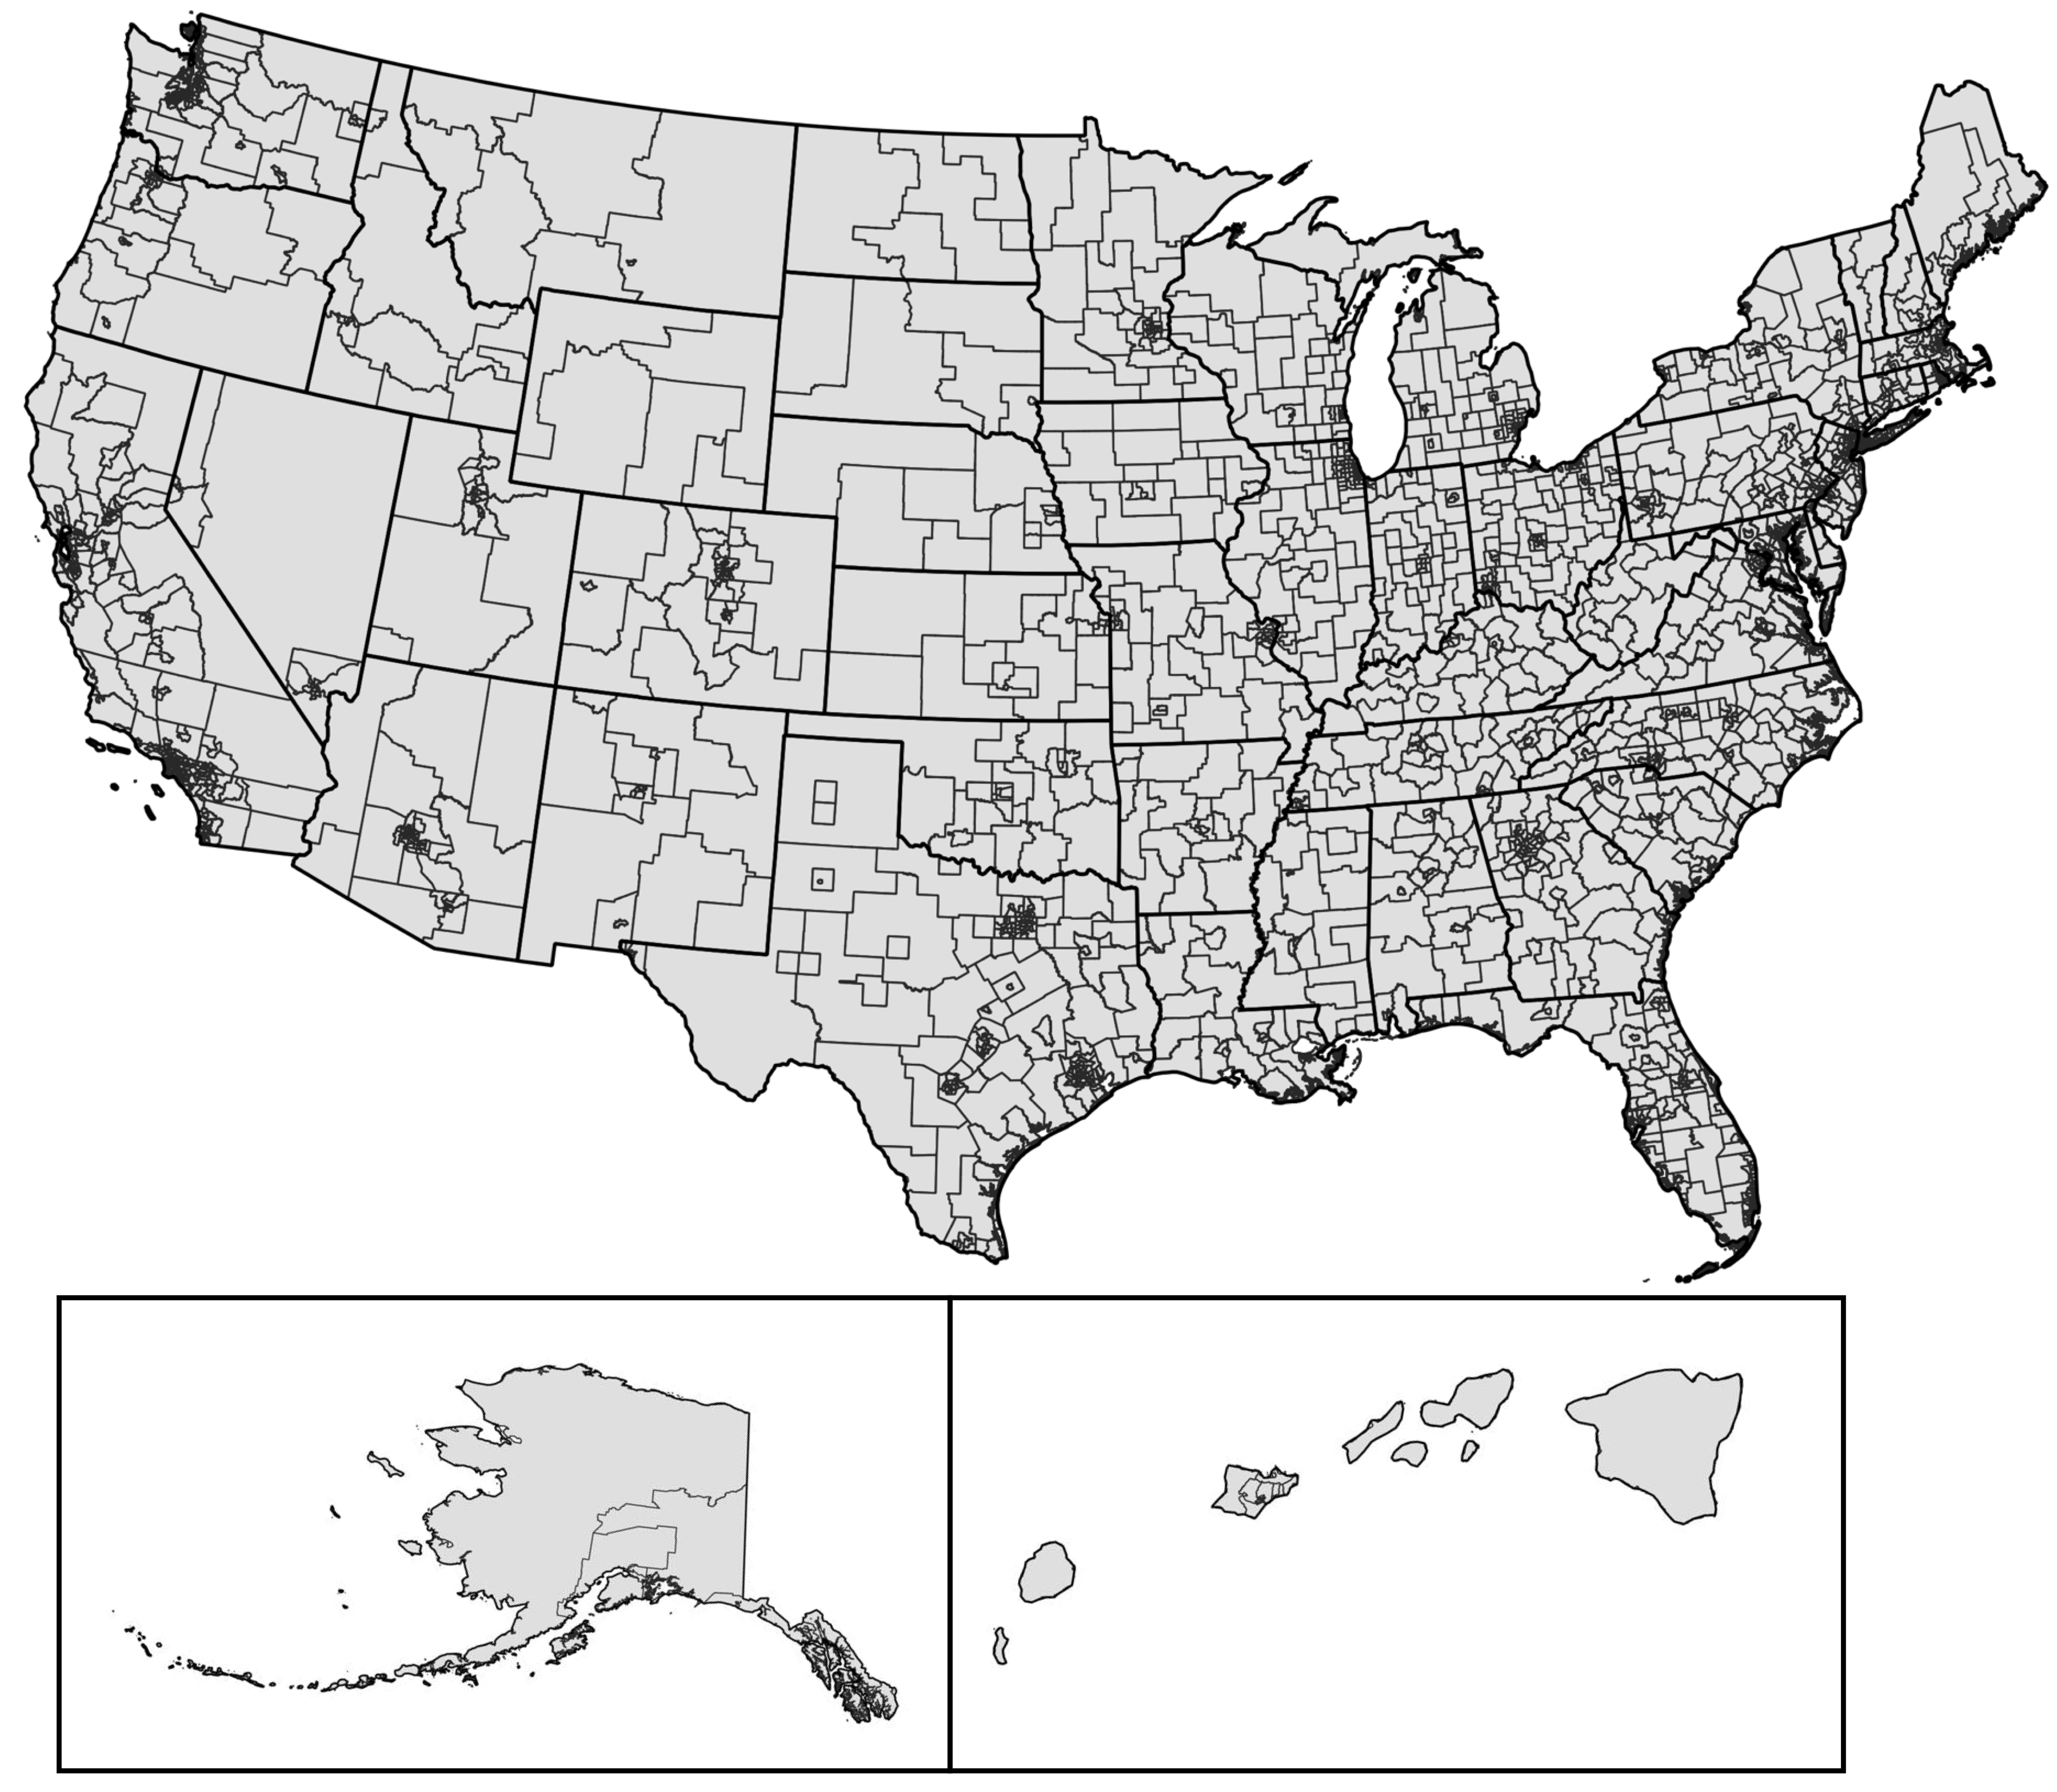
\includegraphics[width=1\linewidth]{images/2010-PUMAs.png}
    \caption{2010 Public Use Microdata Area boundaries}
    \label{fig:2010_puma_boundaries}
\end{figure}

\paragraph{Distribution Data Source(s)}
\begin{itemize} 
\item
  Spatial definitions are from the U.S.~Census Bureau as of July 1,
  2015.
\item
  Unit counts are from the American Community Survey 5-year 2016.
\end{itemize}
\paragraph{Direct Conditional Dependencies}
\begin{itemize}
    \item County and PUMA.
\end{itemize}
\paragraph{Options}
The options for PUMAs are structured by their state abbreviation and the PUMA code from the GISJOIN code. The GISJOIN values are found in the 2010 TIGER/LINE Basis file on the \href{https://usa.ipums.org/usa/volii/boundaries.shtml}{IPUMS GIS Boundary Files}  website. An example is G01002100, which represents state FIPS code AL, and 02100 is the AL, Elmore, Autauga, Montgomery -Outer- and Lowndes Counties PUMA.

There are three ResStock arguments set with the PUMA options: \texttt{site\_elevation}, \texttt{site\_latitude}, and \texttt{site\_longitude}. All three of these arguments are set to ``auto'' and use the default \href{https://openstudio-hpxml.readthedocs.io/en/v1.8.1/workflow_inputs.html#hpxml-building-site}{OpenStudio-HPXML Building Site} values.

\begin{longtable}[]{ |p{3.cm}|p{1.5cm}|p{1cm}|p{1.1cm}|p{1.4cm}|p{6cm}| }
\caption{The ResStock argument definitions set in the PUMA characteristic} \label{table:hc_arg_def_puma}  \\
\toprule\noalign{}
Name & Required & Units & Type & Choices & Description \\
\midrule\noalign{}
\endhead
\bottomrule\noalign{}
\endlastfoot
\texttt{site\_elevation} & false & ft & Double & auto & Elevation of the
home address.  \\
\hline
\texttt{site\_latitude} & false & deg & Double & auto & Latitude of the
home address. Must be between -90 and 90. Use negative values for
southern hemisphere.\\
\hline
\texttt{site\_longitude} & false & deg & Double & auto & Longitude of
the home address. Must be between -180 and 180. Use negative values for
the western hemisphere.\\
\end{longtable}

\paragraph{Distribution Assumption(s)}
No assumptions are made.

\subsubsection{County and PUMA}
\paragraph{Description}
The GISJOIN identifier for the County and the PUMA where the sample is located. Since Counties and PUMAs are both a collection of census tracts, often a PUMA is in multiple counties. This characteristic describes the combination of County and PUMA where the sample is located.

\paragraph{Distribution Data Source(s)}
\begin{itemize}
 
\item
  Spatial definitions are from the U.S.~Census Bureau as of July 1,
  2015.
\item
  Unit counts are from the American Community Survey 5-year 2016.
\end{itemize}

\paragraph{Direct Conditional Dependencies}
\begin{itemize}
    \item ASHRAE IECC Climate Zone 2004.
\end{itemize}
\paragraph{Options}
The options for County and PUMA are a combination of the NHGIS GISJOIN Code for the County and the PUMA separated by a comma. An example option is ``G0100010, G01002100''---G0100010 is the County GISJOIN for Autauga County, AL, and G01002100 is the PUMA GISJOIN for the AL, Elmore, Autauga, Montgomery -Outer- and Lowndes Counties PUMA.

\paragraph{Distribution Assumption(s)}
No assumptions are made.

\subsubsection{Metropolitan and Micropolitan Statistical Area}
\paragraph{Description}
The U.S.~Metropolitan Statistical Area (MSA) or Micropolitan Statistical Area (MicroSA) where sample is located. The U.S.~Census defines a set of counties as Core-Based Statistical Areas (CBSAs). These CBSAs are either assigned a MicroSA or combined into a larger MSA. According to the U.S.~Census, each metropolitan statistical area must have at least one urban area of 50,000 or more inhabitants. According to the U.S.~Census, each MicroSA must have at least one urban area of at least 10,000 but less than 50,000 population.

\paragraph{Distribution Data Source(s)}
\begin{itemize}
 
\item
  Spatial definitions are from the U.S.~Census Bureau as of July 1,
  2015.
\item
  Unit counts are from the American Community Survey 5-year 2016.
\item
  County-MSA crosswalk comes from the Quarterly Census of Employment and
  Wages NAICS-based data between 2013 and 2022 by the U.S.~Bureau of Labor
  Statistics
  (\url{https://www.bls.gov/cew/classifications/areas/county-msa-csa-crosswalk.htm}).
\end{itemize}

\paragraph{Direct Conditional Dependencies}
\begin{itemize}
    \item County.
\end{itemize}

\paragraph{Options}
Options of the Metropolitan and Micropolitan Statistical Area characteristic are structured by having the name of the MSA or MicroSA, a comma, the State abbreviation, and either ``MSA'' or ``MicroSA.'' An example is ``Albany-Schenectady-Troy, NY MSA,'' which corresponds to the Albany-Schenectady-Troy MSA in New York State.

\paragraph{Distribution Assumption(s)}
No assumptions are made.

\subsubsection{City}
\paragraph{Description}
The City where the sample is located.

\paragraph{Distribution Data Source(s)}
\begin{itemize}
 
\item
  Spatial definitions are from the U.S.~Census Bureau as of July 1,
  2015.
\item
  Cities are defined by Census blocks by their Census Place in the 2010
  Census.
\item
  Unit counts are from the American Community Survey 5-year 2016.
\end{itemize}

\paragraph{Direct Conditional Dependencies}
\begin{itemize}
    \item County and PUMA.
\end{itemize}

\paragraph{Options}
The options are structured as the State abbreviation of the city, a comma, and the name of the city. An example is ``AR, Jonesboro,'' which corresponds to Jonesboro, Arkansas.

The ResStock argument \texttt{site\_city} is assigned in the City characteristic. The argument is set to ``auto,'' which is the OpenStudio-HPXML default value; see the OpenStudio-HPXML \href{https://openstudio-hpxml.readthedocs.io/en/v1.8.1/workflow_inputs.html#hpxml-building-site}{Building Site} section of the documentation for the default values.

\begin{longtable}[]{ |p{3.cm}|p{1.5cm}|p{1.1cm}|p{6cm}| }
\caption{The ResStock argument definitions set in the City characteristic} \label{table:hc_arg_def_city}  \\
\toprule\noalign{}
Name & Required & Type  & Description \\
\midrule\noalign{}
\endhead
\bottomrule\noalign{}
\endlastfoot
\texttt{site\_city} & false & String & City/municipality of the home
address. \\
\end{longtable}

\paragraph{Distribution Assumption(s)}
\begin{itemize}
\item
  2020 Decennial Redistricting data were used to map tract-level unit
  counts to census blocks.
\item
  1,099 cities are tagged in ResStock, but there are over 29,000 Places
  in the Census data.
\item
  The threshold for including a Census Place in the City characteristic is 15,000 housing units.
\item
  The value ``In Another Census Place'' designates the fraction of housing units in a Census Place with fewer total housing units than the threshold.
\item
  The value ``Not in a Census Place''
  designates the fraction of housing units not in a Census Place
  according to the 2010 Census.
\end{itemize}


\subsubsection{AIANNH Area}
\paragraph{Description}
American Indian/Alaska Native/Native Hawaiian (AIANNH) Area where the sample is located. See Figure \ref{fig:aiannh_map} for a map of AIANNH areas in the contiguous United States.

\begin{figure}
    \centering
    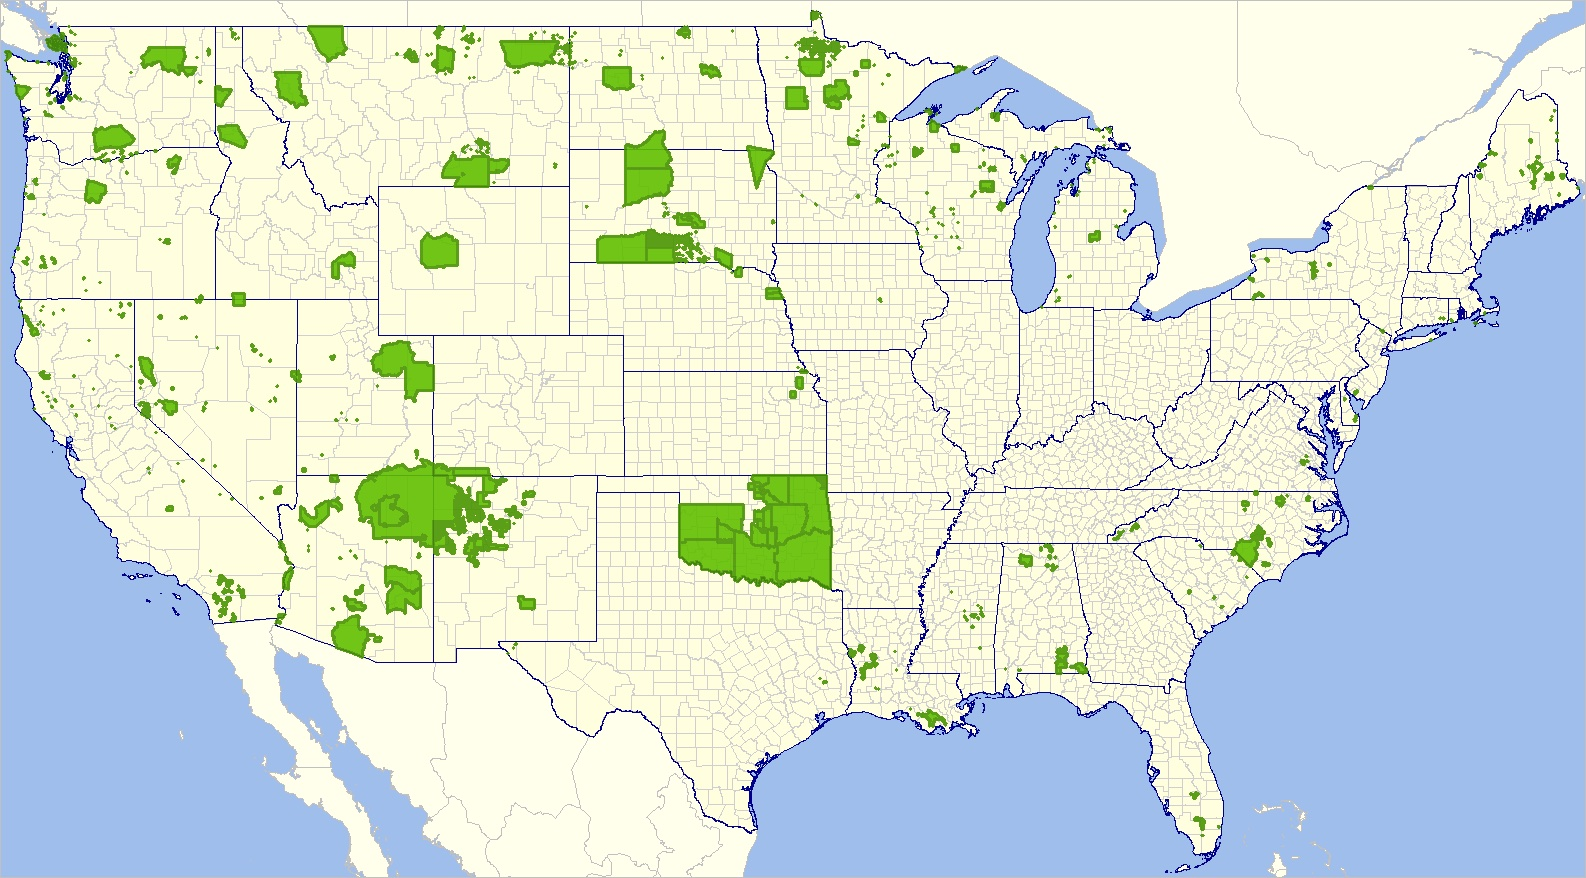
\includegraphics[width=1\linewidth]{images/aiannh_48b.jpg}
    \caption{AIANNH area map. The image is created by \href{https://proximityone.com/aiannh.htm}{ProximityOne} and excludes Alaska and Hawaii.}
    \label{fig:aiannh_map}
\end{figure}


\paragraph{Distribution Data Source(s)}
\begin{itemize}
    \item 2010 Census Tract to American Indian Area (AIA) Relationship File provides the percent housing units in the census tract that belong to AIA. 
    \item Spatial definitions are from the U.S.~Census Bureau as of July 1, 2015.
    \item Unit counts are from the American Community Survey 5-year 2016.
\end{itemize}

\paragraph{Direct Conditional Dependencies}
\begin{itemize}
    \item County and PUMA.
\end{itemize}

\paragraph{Options}
The options are either ``Yes'' or ``No,'' indicating if the housing unit is in an AIANNH area.

\paragraph{Distribution Assumption(s)}
\begin{itemize}
    \item The 2010 Census Tracts are mapped to 2015 County and PUMA by adjusting for known geographic changes (e.g., renaming of Shannon County to Oglala Lakota County, SD) However, Tract=G3600530940103 (Oneida city, Madison County, NY) could not be mapped to County and PUMA and was removed. The tract contains only 11 units for AIA.
\end{itemize}

\subsubsection{County Metro Status}
\paragraph{Description}
The Metro Status of the county where the sample is located and is based on MSA and MicroSA.

\paragraph{Distribution Data Source(s)}
\begin{itemize}
    \item Spatial definitions are from the U.S.~Census Bureau as of July 1, 2015.
    \item Unit counts are from the American Community Survey 5-year 2016.
    \item County-MSA crosswalk comes from the Quarterly Census of Employment and Wages NAICS-based data between 2013 and 2022 by the  \href{https://www.bls.gov/cew/classifications/areas/county-msa-csa-crosswalk.htm}{U.S.~Bureau of Labor Statistics}.
\end{itemize}

\paragraph{Direct Conditional Dependencies}
\begin{itemize}
    \item Metropolitan and Micropolitan Statistical Area.
\end{itemize}

\paragraph{Options}
The options are either ``Metropolitan'' or ``Non-Metropolitan.''

\paragraph{Distribution Assumption(s)}
No assumptions are made.


\subsubsection{PUMA Metro Status}
\paragraph{Description}
The PUMA metropolitan status where the housing unit is located.

\paragraph{Distribution Data Source(s)}
\begin{itemize}
    \item 2019 5-year PUMS from the University of Minnesota.
\end{itemize}

\paragraph{Direct Conditional Dependencies}
\begin{itemize}
    \item PUMA.
\end{itemize}

\paragraph{Options}
The options are either (1) In metro area, not/partially in principal city, (2) In metro area, principal city, or (3) Not/partially in metro area. 

\paragraph{Distribution Assumption(s)}
\begin{itemize}
    \item The PUMA Metro Status, derived from ACS IPUMS METRO codes, indicates whether the household resided within a metropolitan area and, for households in metropolitan areas, whether the household resided within or outside of a central/principal city. Each PUMA has a unique METRO status in ACS and therefore has a unique PUMA Metro Status. IPUMS derives METRO codes for samples not directly identified based on available geographic information and whether the associated county group or PUMA lies wholly or only partially within metropolitan areas or principal cities.
\end{itemize}

\subsection{Climate Zones}
This section of ResStock characteristics is a set of climate zone definitions. There are five input files to ResStock that specify climate zones:
\begin{itemize}
    \item ASHRAE IECC Climate Zone 2004
    \item ASHRAE IECC Climate Zone 2004---2A Split
    \item Building America Climate Zones
    \item California Energy Commission (CEC) Climate Zones
    \item ENERGY STAR\textsuperscript{\textregistered} Climate Zone 2023.
\end{itemize}
\subsubsection{ASHRAE IECC Climate Zone 2004} \label{sec:ashrae_2004_tsv}
\paragraph{Description}
Climate zone according to ASHRAE 169 in 2004 and IECC in 2012 where the sample is located. See Figure \ref{fig:ashrae_169_2004_cz} for a map of the climate zones.

\begin{figure}
    \centering
    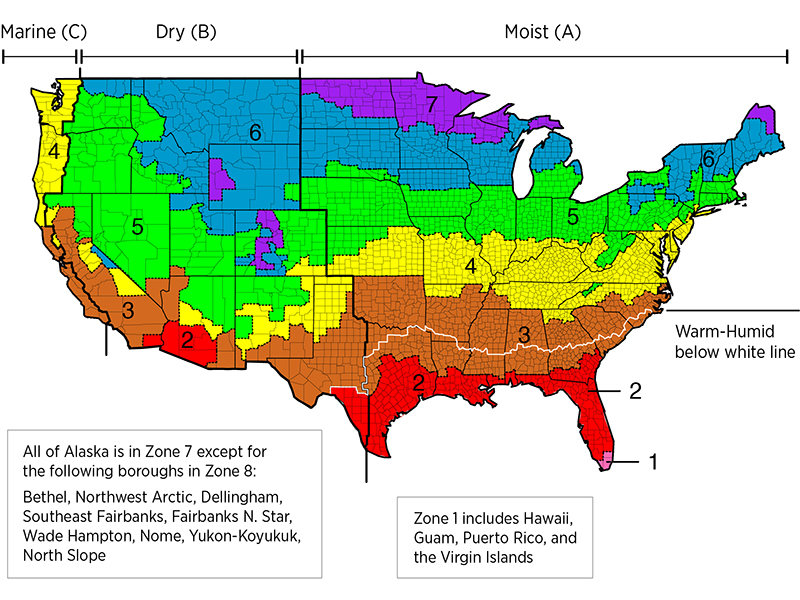
\includegraphics[width=1\linewidth]{images/ashrae_iecc_cz_map_2004.jpg}
    \caption{The 2004 ASHRAE 169 and IECC 2012 climate zone map}
    \label{fig:ashrae_169_2004_cz}
\end{figure}

\paragraph{Distribution Data Source(s)}
\begin{itemize}
    \item Spatial definitions are from the U.S.~Census Bureau as of July 1, 2015.
    \item Unit counts are from the American Community Survey 5-year 2016.
    \item Climate zone data are from ASHRAE 169 2004, IECC 2012, and \href{https://www.energy.gov/sites/prod/files/2015/10/f27/ba_climate_region_guide_7.3.pdf}{M.C. Baechler 2015}.
\end{itemize}

\paragraph{Direct Conditional Dependencies}
There are no direct conditional dependencies.

\paragraph{Options}
A set of counties defines each climate and moisture zone. Climate zones range from 1--8 and moisture zones are indicated by A, B, and C. 

The ASHRAE IECC Climate Zone 2004 sets the \texttt{site\_type} and \texttt{site\_iecc\_zone} arguments. The \texttt{site\_type} is always set to ``auto.'' The \texttt{site\_iecc\_zone} argument matches the climate zone with the exception of climate zones 7 and 8 in Alaska. ResStock departs from the climate zone definitions by using 7AK and 8AK instead of 7 and 8 from the standards.

\begin{customLongTable}{ |p{3.cm}|p{1.5cm}|p{1.1cm}|p{4.4cm}|p{4cm}| }
{The ResStock arguments set in the ASHRAE IECC Climate Zone 2004 characteristic} {table:hc_arg_def_ashrae_2004}  
{Name & Required & Type & Choices & Description} 
\texttt{site\_type} & false & Choice & auto, suburban, urban, rural &
The type of site.  \\
\hline
\texttt{site\_iecc\_zone} & false & Choice & auto, 1A, 1B, 1C, 2A, 2B,
2C, 3A, 3B, 3C, 4A, 4B, 4C, 5A, 5B, 5C, 6A, 6B, 6C, 7, 8 & IECC zone of
the home address. \\
\end{customLongTable}

\paragraph{Distribution Assumption(s)}
No assumptions are made.

\subsubsection{ASHRAE IECC Climate Zone 2004---2A Split}
\paragraph{Description}
The climate zone, according to ASHRAE 169 in 2004 and IECC in 2012, where the sample is located. Climate zone where climate zone 2A is split between counties in (1) TX and LA, and (2) FL, GA, AL, and MS. See Figure \ref{fig:ashrae_169_2004_cz} for the climate zones and the climate zone 2A counties that are split between the states mentioned previously.

\paragraph{Distribution Data Source(s)}
\begin{itemize}
    \item Spatial definitions are from the U.S.~Census Bureau as of July 1, 2015.
    \item Unit counts are from the American Community Survey 5-year 2016.
    \item Climate zone data are from ASHRAE 169 2004, IECC 2012, and \href{https://www.energy.gov/sites/prod/files/2015/10/f27/ba_climate_region_guide_7.3.pdf}{M.C. Baechler 2015}.
\end{itemize}

\paragraph{Direct Conditional Dependencies}
\begin{itemize}
    \item County.
\end{itemize}

\paragraph{Options}
A set of counties defines each climate and moisture zone. Climate zones range from 1--8 and moisture zones are indicated by A, B, and C. Climate zone 2A is split between options ``2A---FL, GA, AL, MS'' and ``2A---TX, LA.''

\paragraph{Distribution Assumption(s)}
\begin{itemize}
    \item This characteristic is used to better represent HVAC types in the 2A climate zone.
\end{itemize}

\subsubsection{Building America Climate Zones}
\paragraph{Description}
The Building America Climate Zone where the sample is located. See Figure \ref{fig:building_america_cz} for a map of the climate zones.\footnote{The Subarctic climate zone is not shown and is only found in Alaska.}

\begin{figure}
    \centering
    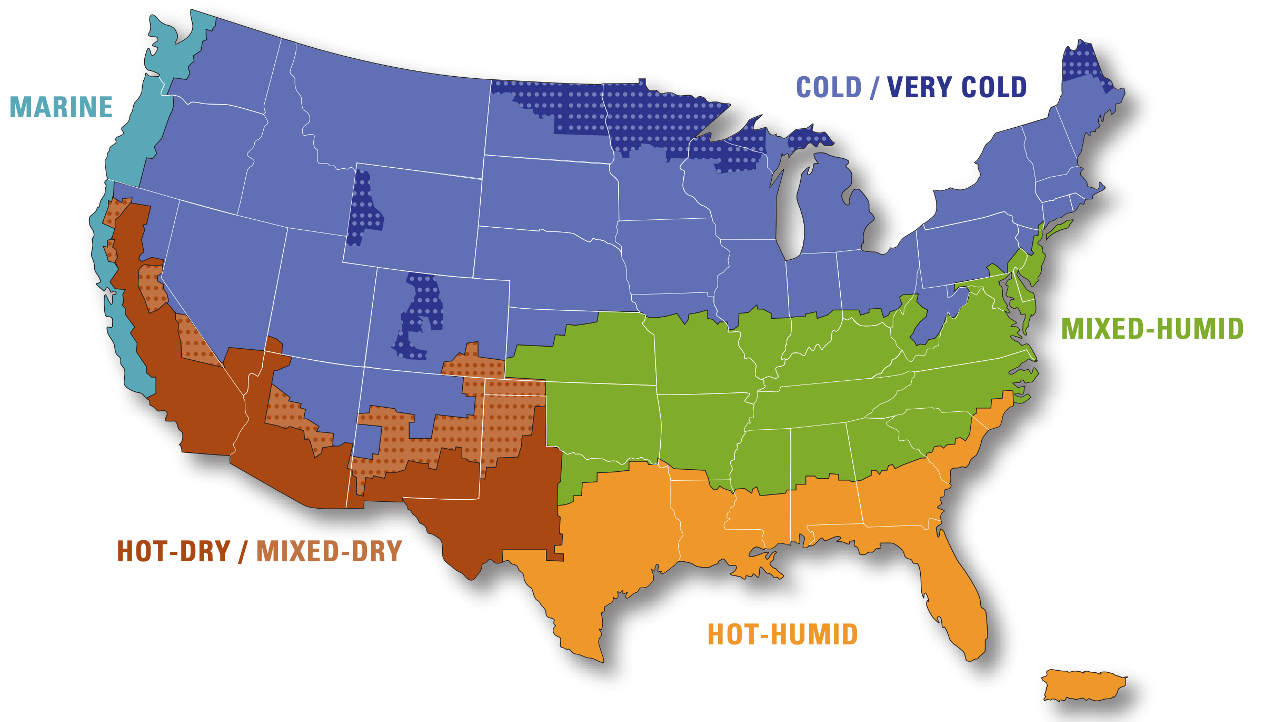
\includegraphics[width=1\linewidth]{images/building_america_cz.png}
    \caption{Building America Climate Zone map}
    \label{fig:building_america_cz}
\end{figure}

\paragraph{Distribution Data Source(s)}
\begin{itemize}
    \item Unit counts are from the American Community Survey 5-year 2016.
    \item Spatial definitions are from U.S.~Census 2010.
    \item Climate zone data are from ASHRAE 169 2004, IECC 2012, and \href{https://www.energy.gov/sites/prod/files/2015/10/f27/ba_climate_region_guide_7.3.pdf}{M.C. Baechler 2015}.
\end{itemize}

\paragraph{Direct Conditional Dependencies}
\begin{itemize}
    \item County.
\end{itemize}

\paragraph{Options}
The options for the Building America Climate Zone characteristic are the same as the climate zones: Cold, Hot-Dry, Hot-Humid, Marine, Mixed-Dry, Mixed-Humid, Subarctic, and Very Cold.

\paragraph{Distribution Assumption(s)}
No assumptions are made.

\subsubsection{California Energy Commission Climate Zones}
\paragraph{Description}
The CEC Climate Zone where the sample is located. See Figure \ref{fig:cec_cz} for a map of the CEC building climate zones.

\begin{figure}
    \centering
    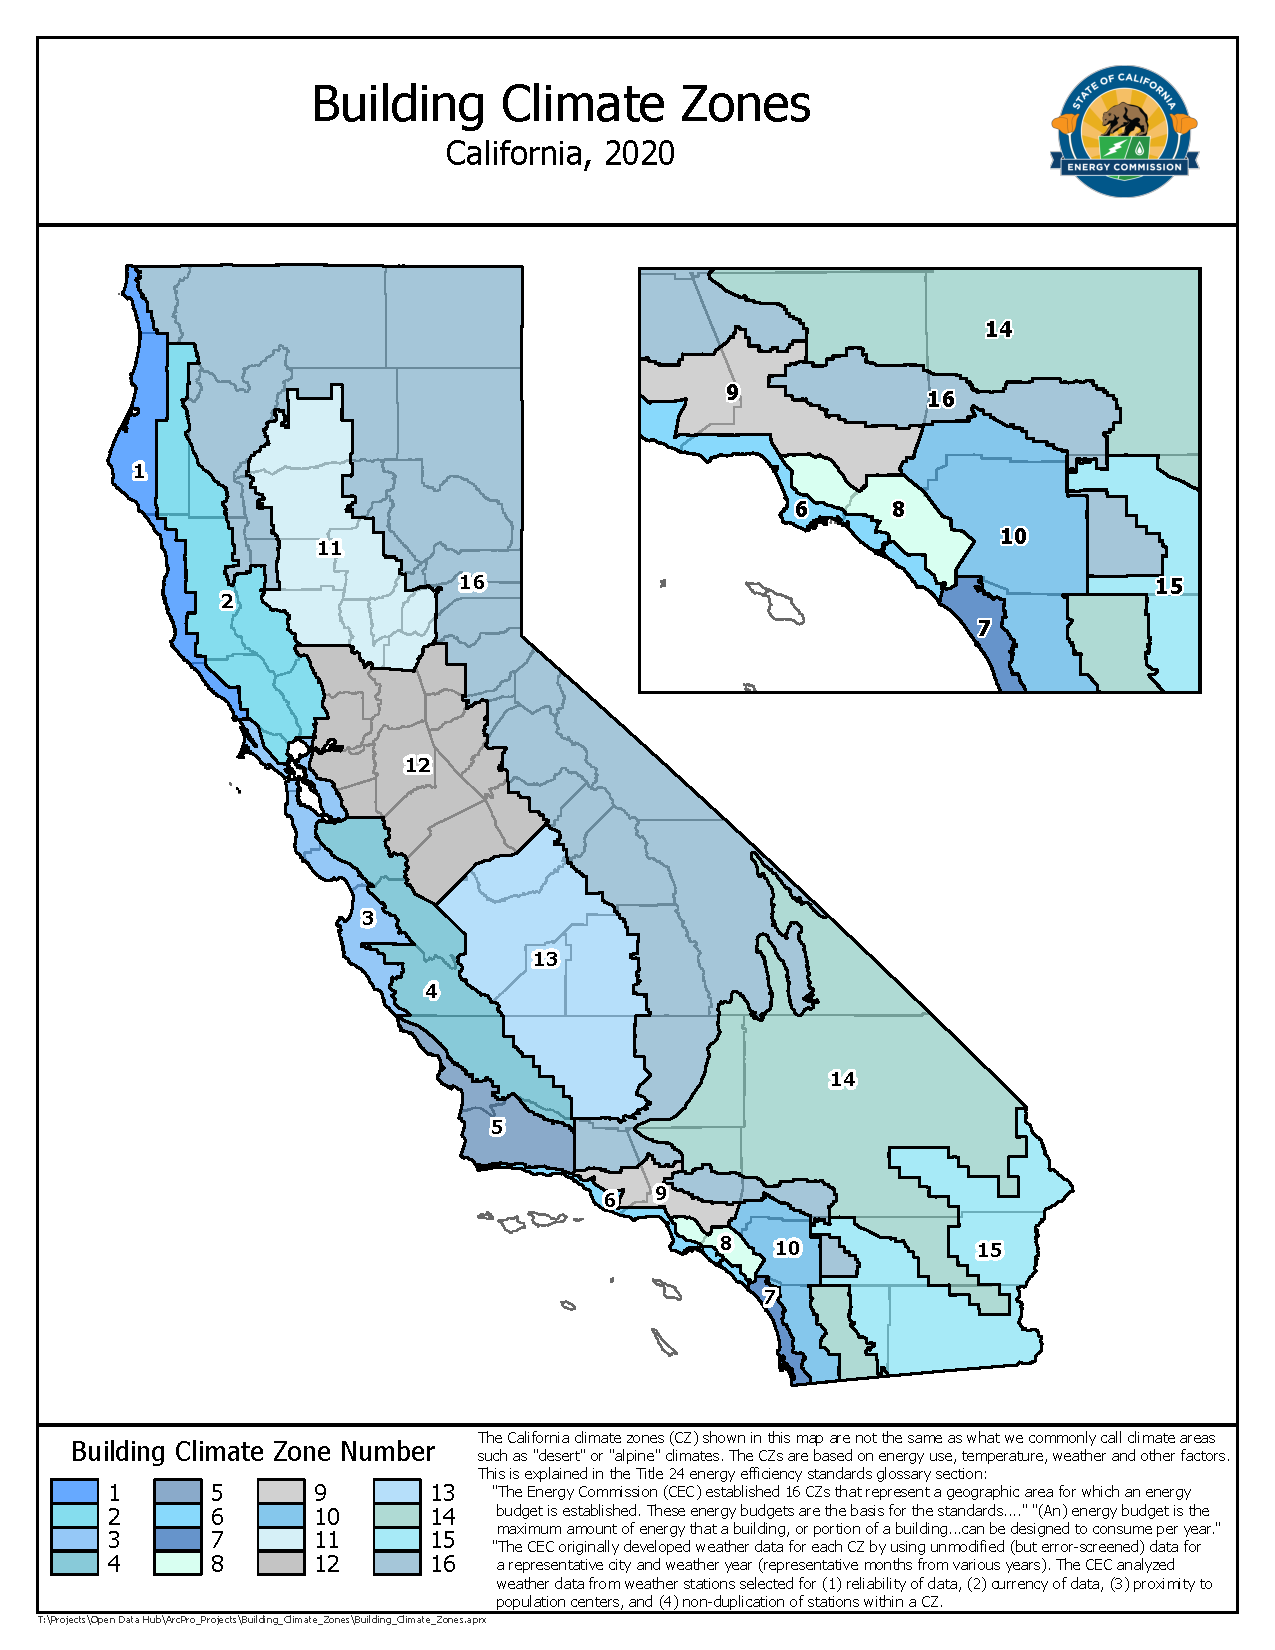
\includegraphics[width=1\linewidth]{images/CEC_Building_Climate_Zones.pdf}
    \caption{California Energy Commission \href{https://cecgis-caenergy.opendata.arcgis.com/documents/CAEnergy::building-climate-zones/explore}{Building Climate Zone map}}
    \label{fig:cec_cz}
\end{figure}

\paragraph{Distribution Data Source(s)}
\begin{itemize}
    \item Spatial definitions are from the U.S.~Census Bureau as of July 1, 2015.
    \item Zip code definitions are from the end of Q2 2020.
    \item The climate zone to zip codes in California are from the CEC website.
\end{itemize}

\paragraph{Direct Conditional Dependencies}
\begin{itemize}
    \item County and PUMA.
\end{itemize}

\paragraph{Options}
The options range from 1--16 in California. For other states, the option is set to None.

\paragraph{Distribution Assumption(s)}
\begin{itemize}
    \item CEC Climate zones are defined by zip codes.
    \item The dependency selected is County and PUMA as zip codes are not modeled in ResStock.
    \item The mapping between Census Tracts and zip codes is approximate and some discrepancies may exist.
\end{itemize}

\subsubsection{ENERGY STAR Climate Zone 2023}
\paragraph{Description}
Climate zones for windows, doors, and skylights per ENERGY STAR guidelines as of 2023. See Figure \ref{fig:energy_star_cz} for a map of the climate zones.

\begin{figure}
    \centering
    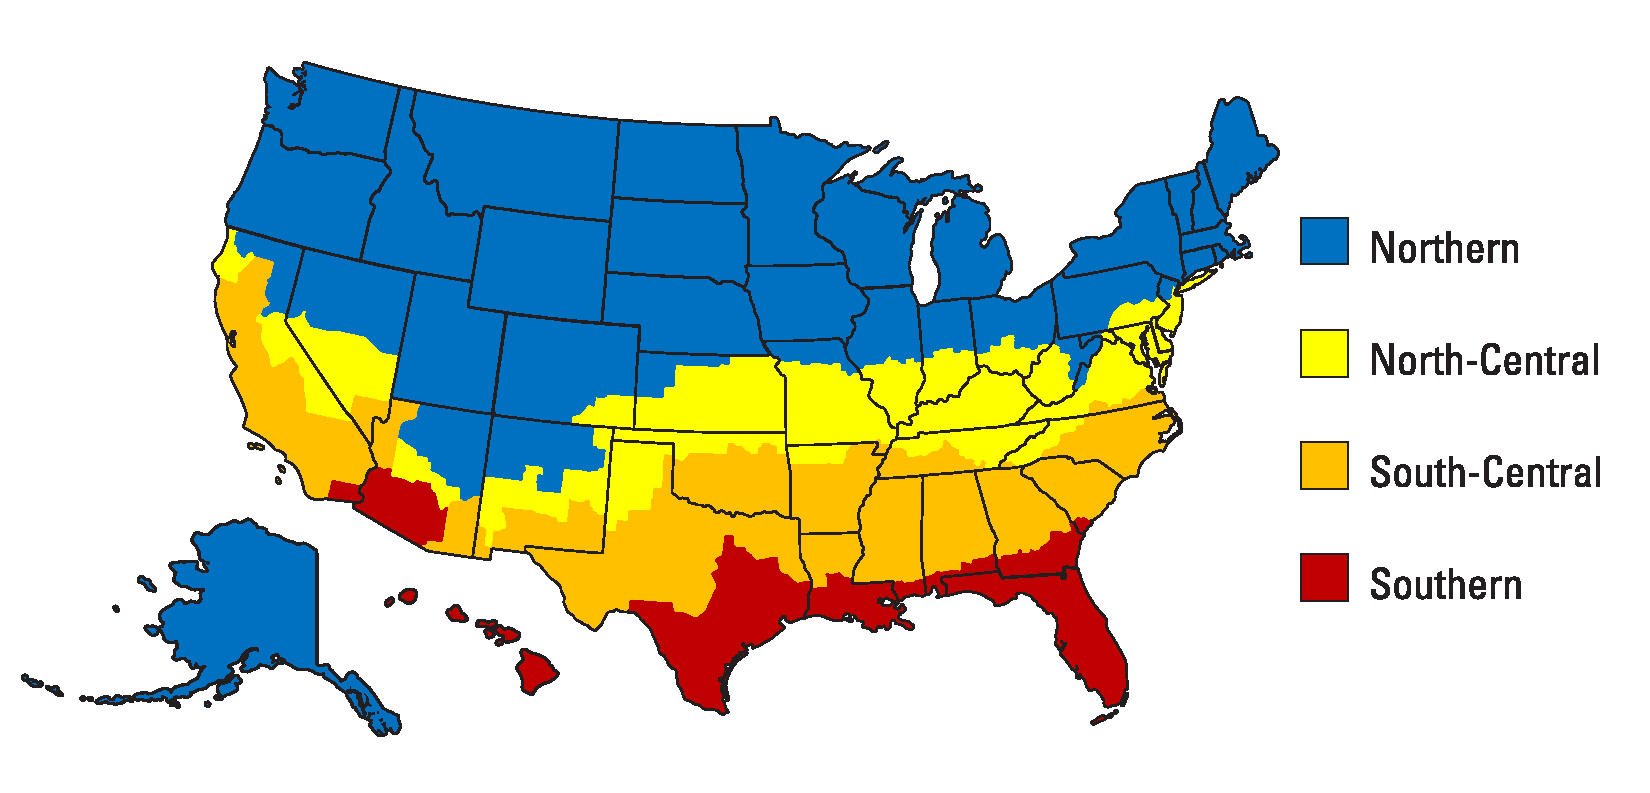
\includegraphics[width=1\linewidth]{images/ENERGY_STAR_Climate_Zone_Map.pdf}    \caption{\href{https://www.energystar.gov/sites/default/files/asset/document/Promotional_Map.pdf}{ENERGY STAR V7 climate zone} map}
    \label{fig:energy_star_cz}
\end{figure}

\paragraph{Distribution Data Source(s)}
\begin{itemize}
    \item Area definition approximated based on published map retrieved in May 2023 from the \href{https://www.energystar.gov/products/residential_windows_doors_and_skylights/key_product_criteria}{ENERGY STAR windows, doors, and skylights key product criteria} website. 
\end{itemize}

\paragraph{Direct Conditional Dependencies}
\begin{itemize}
    \item CEC Climate Zone
    \item County.
\end{itemize}

\paragraph{Options}
The options for the ENERGY STAR Climate Zone 2023 characteristic are the same as climate zones: North-Central, Northern, South-Central, and Southern. 

\paragraph{Distribution Assumption(s)}
\begin{itemize}
    \item ENERGY STAR Climate Zones assigned based on CEC Climate Zone for California and based on County everywhere else.
\end{itemize}

\subsection{Grid and Emissions Geographies}

In ResStock there are three input files describing geographies relevant to the electric grid and emissions calculations:

\begin{itemize}
    \item ReEDS Balancing Area
    \item Generation and Emissions Assessment (GEA) Region
    \item ISO RTO Region.
\end{itemize}

\subsubsection{ReEDS Balancing Area}
\paragraph{Description}
The Regional Energy Deployment System Model (ReEDS) balancing area where the sample is located. See Figure \ref{fig:reeds_ba_map} to see a map of the balancing areas.

\begin{figure}
    \centering
    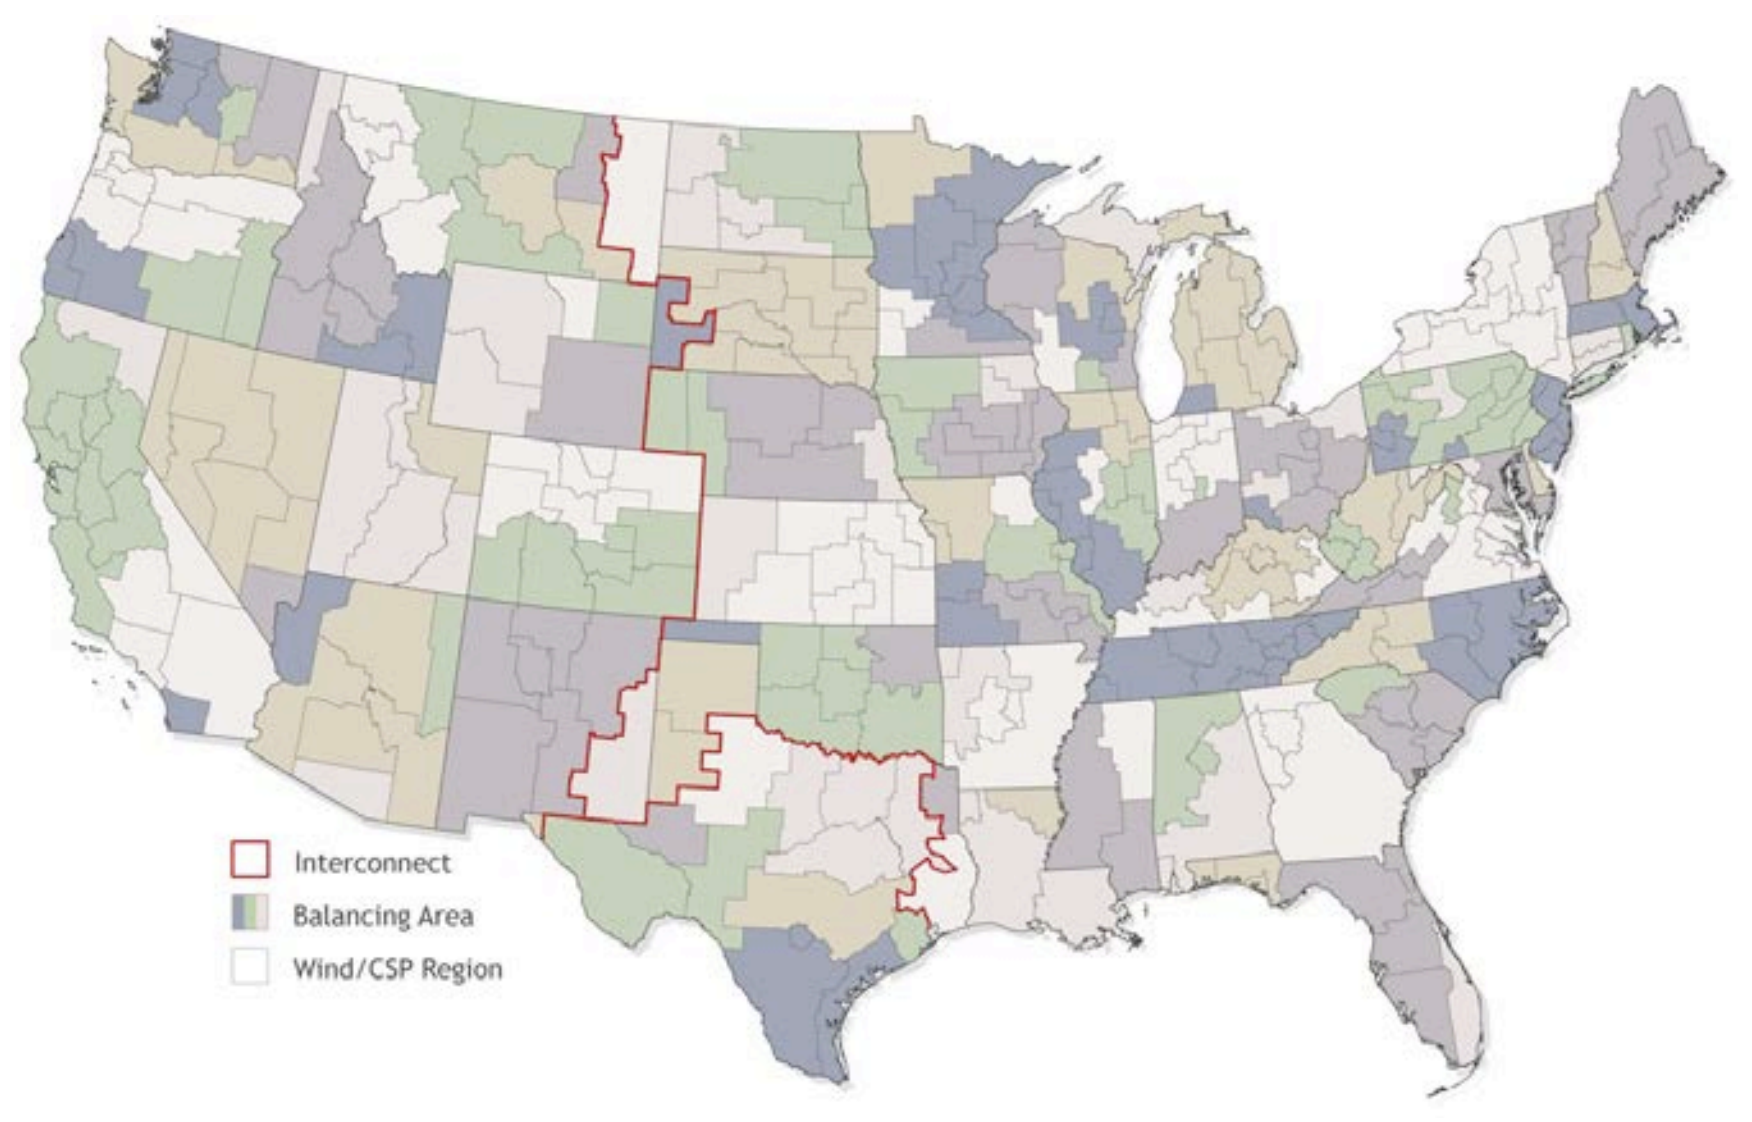
\includegraphics[width=1\linewidth]{images/reeds_ba_map.png}
    \caption{ReEDS balancing area map}
    \label{fig:reeds_ba_map}
\end{figure}

\paragraph{Distribution Data Source(s)}
\begin{itemize}
    \item Spatial definitions are from the U.S.~Census Bureau as of July 1, 2015.
    \item Unit counts are from the American Community Survey 5-year 2016.
    \item Regional Energy Deployment System (ReEDS) Model Documentation: Version 2019 (\cite{Brown2019})
    

\end{itemize}

\paragraph{Direct Conditional Dependencies}
\begin{itemize}
    \item County.
\end{itemize}
\paragraph{Options}
The options for the ReEDS Balancing Area characteristic is a set of integers 1-134 based on Figure \ref{fig:reeds_ba_map}. Alaska and Hawaii do not have a ReEDS balancing area and are labeled with the None option.
\paragraph{Distribution Assumption(s)}
No assumptions are made.

\subsubsection{Generation and Emissions Assessment (GEA) Region}
\paragraph{Description}
The 2021 Cambium generation and carbon emissions assessment region where the sample is located. See Figure \ref{fig:cambium_gea_map} for a map of these regions.

\begin{figure}
    \centering
    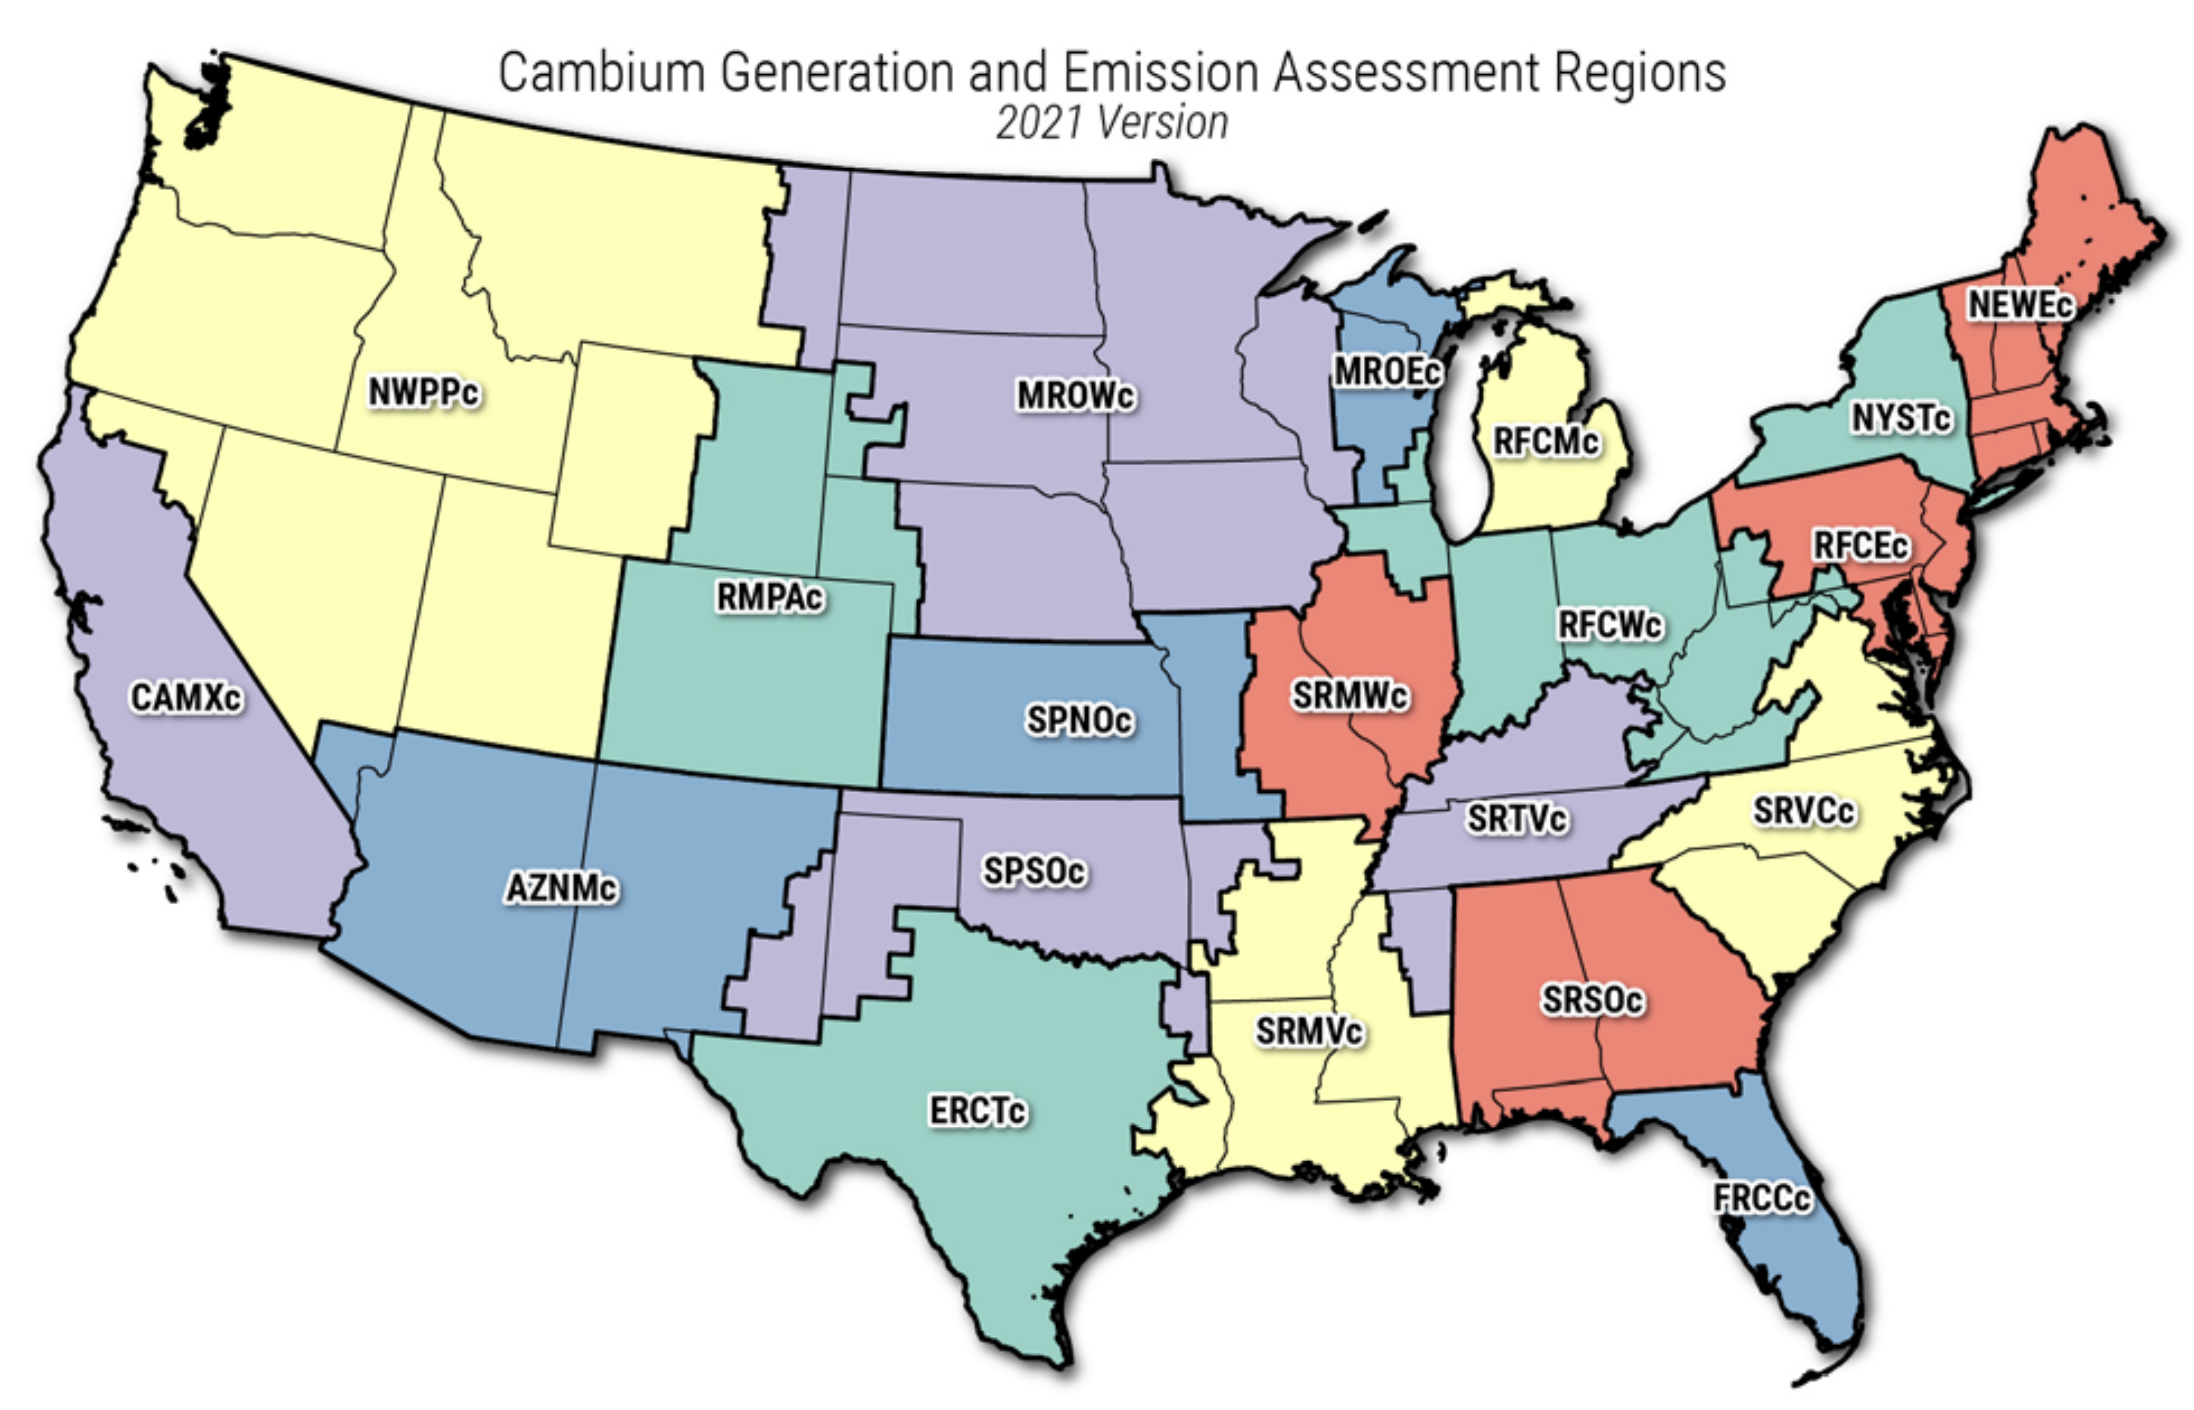
\includegraphics[width=1\linewidth]{images/Cambium_GEAs_2021.png}
    \caption{ Map of the \href{https://www.nrel.gov/analysis/cambium.html}{Cambium} 2021 Generation and Emission Assessment Regions}
    \label{fig:cambium_gea_map}
\end{figure}

\paragraph{Distribution Data Source(s)}
\begin{itemize}
    \item Cambium Documentation: Version 2021 (\cite{Gagnon2021}).

\end{itemize}

\paragraph{Direct Conditional Dependencies}
\begin{itemize}
    \item REEDS Balancing Area.
\end{itemize}

\paragraph{Options}
The options follow the Cambium GEA region names: AZNMc, CAMXc, ERCTc, FRCCc, MROEc, MROWc, NEWEc, NWPPc, NYSTc, RFCEc, RFCMc, RFCWc, RMPAc, SPNOc, SPSOc, SRMVc, SRMWc, SRSOc, SRTVc, and SRVCc. The None option is set for Alaska and Hawaii as these states do not have a ReEDS balancing area.

\paragraph{Distribution Assumption(s)}
No assumptions are made.

\subsubsection{ISO RTO Region}
\paragraph{Description}
The independent system operator (ISO) or regional transmission organization (RTO) region where the sample is located.

\paragraph{Distribution Data Source(s)}
\begin{itemize}
    \item Spatial definitions are from the U.S.~Census Bureau as of July 1, 2015.
    \item Unit counts are from the American Community Survey 5-year 2016.
    \item ISO and RTO regions are from EIA Form 861, 2018.
\end{itemize}

\paragraph{Direct Conditional Dependencies}
\begin{itemize}
    \item County
\end{itemize}

\paragraph{Options}
The options are a list of options that represent ISOs and RTOs:
\begin{itemize}
    \item Pennsylvania New Jersey Maryland Interconnection (PJM)
    \item Midcontinent Independent System Operator (MISO)
    \item Electric Reliability Council of Texas (ERCOT)
    \item California ISO (CAISO)
    \item New York ISO (NYISO)
    \item Southwest Power Pool (SPP)
    \item ISO New England (NEISO).
\end{itemize}
If the county is not in any of these regions, the option is listed as the None option.

\paragraph{Distribution Assumption(s)}
No assumptions were made.

\subsection{Other Geographies}

In this section, we cover other miscellaneous geographies in ResStock. This includes four input files:
\begin{itemize}
    \item Census Division RECS
    \item Custom State
    \item Location Region
    \item American Housing Survey Region.
\end{itemize}

\subsubsection{Census Division RECS}
\paragraph{Description}
Census Division as used in RECS 2015 where the sample is located.

\paragraph{Distribution Data Source(s)}
\begin{itemize}
    \item Spatial definitions are from the U.S.~Census Bureau as of July 1, 2015.
    \item Unit counts are from the American Community Survey 5-year 2016.
    \item U.S.~EIA 2015 RECS codebook.
\end{itemize}

\paragraph{Direct Conditional Dependencies}
\begin{itemize}
    \item State.
\end{itemize}

\paragraph{Options}
The options match the names of the Census divisions except for RECS 2015 splits the Mountain Census Division into North (CO, ID, MT, UT, WY) and South (AZ, NM, NV).

\paragraph{Distribution Assumption(s)}
No assumptions were made.

\subsubsection{Custom State}
\paragraph{Description}
A custom selection of states to be able to have more fine-tuned probability distribution in states where we have more data.

\paragraph{Distribution Data Source(s)}
No data sources were used.

\paragraph{Direct Conditional Dependencies}
\begin{itemize}
    \item State.
\end{itemize}
\paragraph{Options}
The options for the Custom State characteristic are ``AK'' and ``Others.'' The characteristic was added during the calibration of Alaska to integrate the Alaska Retrofit Information System data.

\paragraph{Distribution Assumption(s)}
No assumptions were made.

\subsubsection{Location Region}
\paragraph{Description}
A custom ResStock region constructed of EIA RECS 2009 reportable domains where the sample is located. See Figure \ref{fig:location_region_map} for a map of these regions.

\begin{figure}
    \centering
    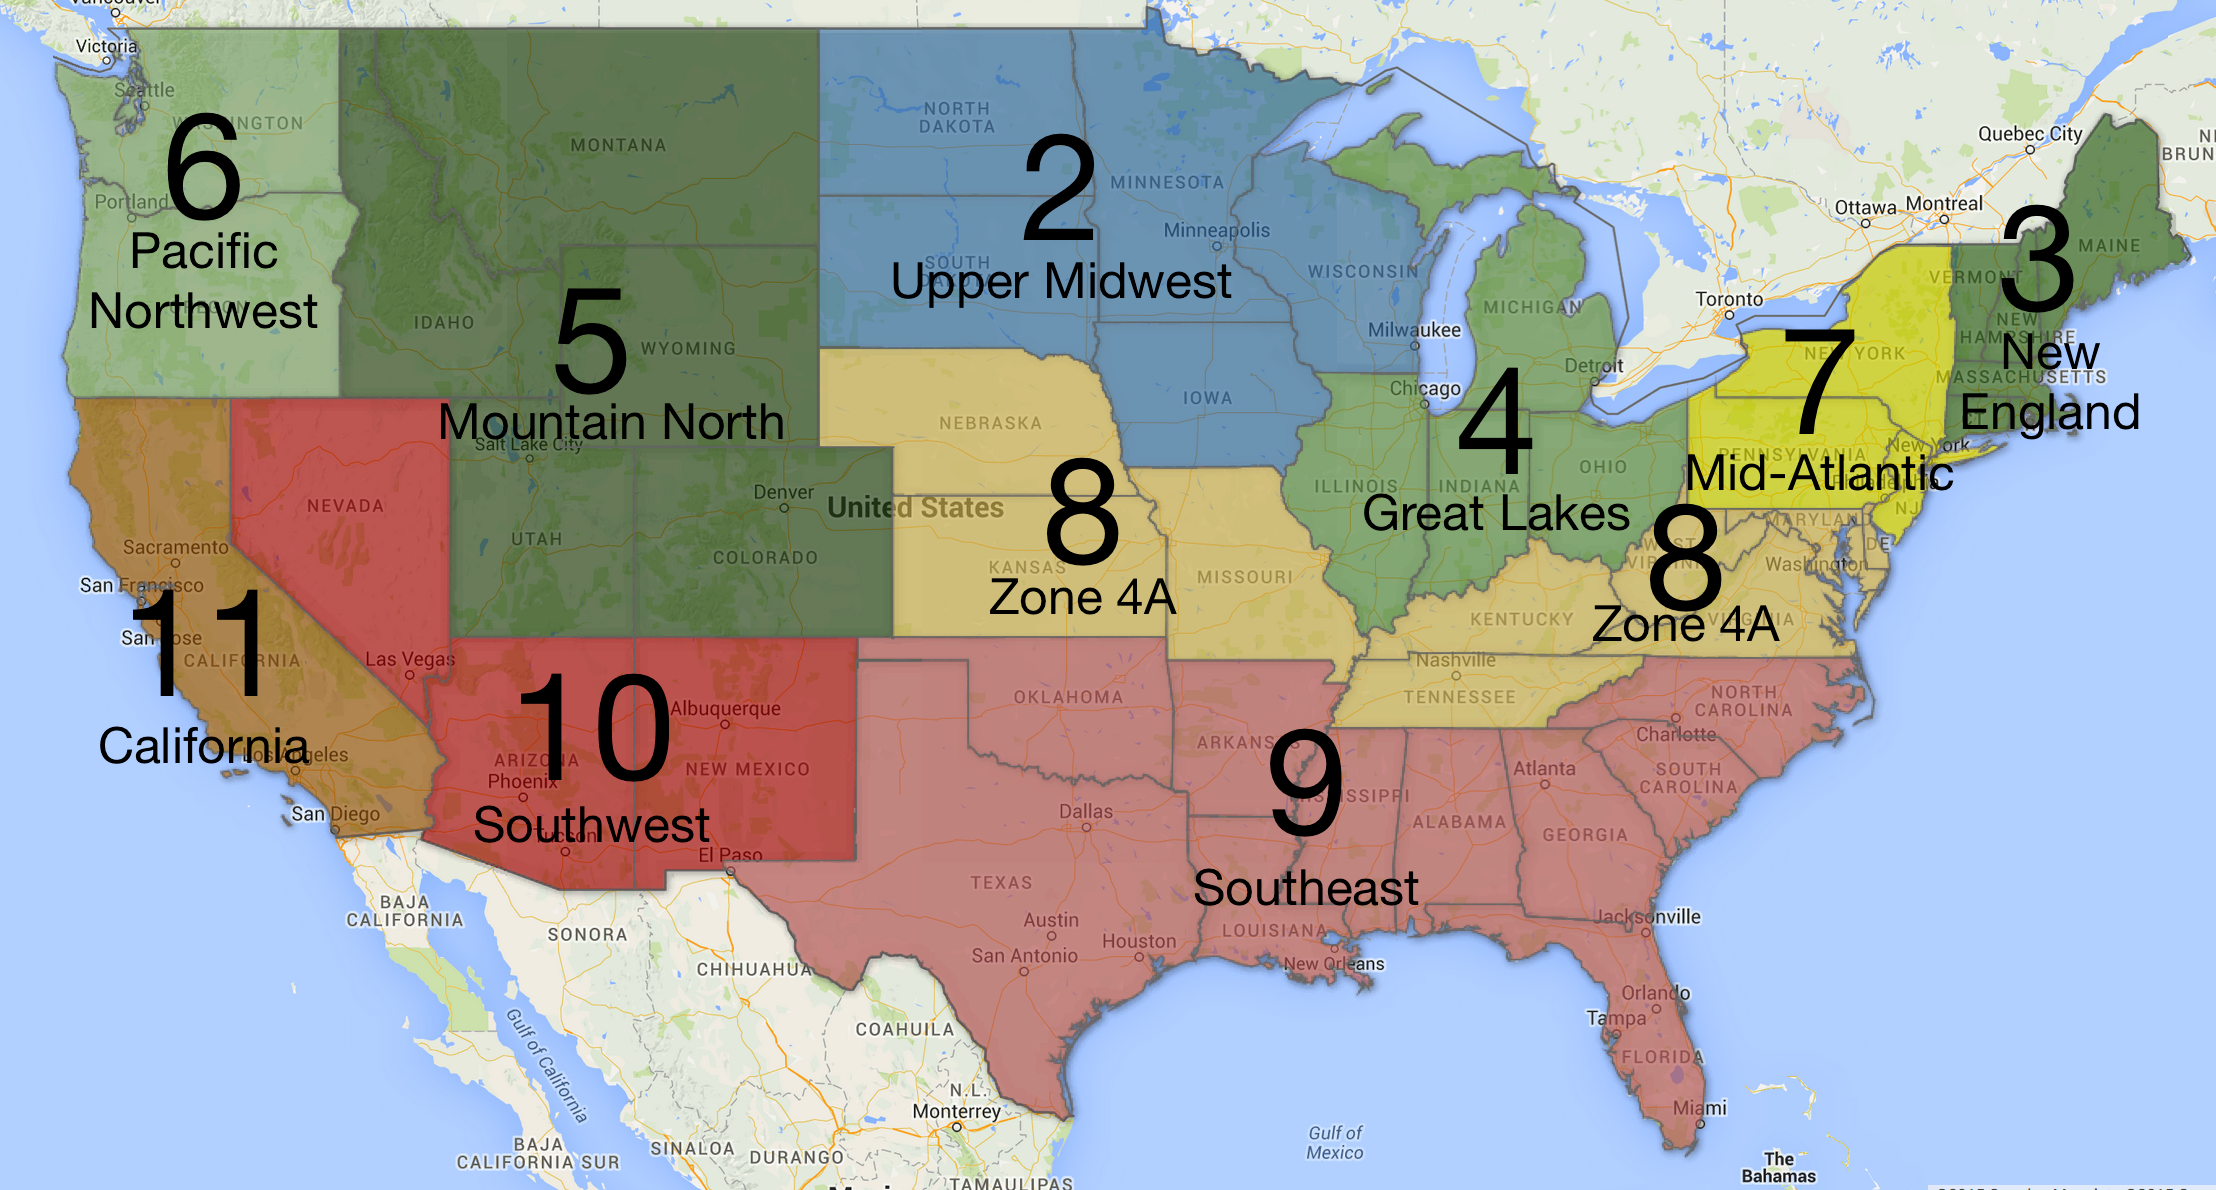
\includegraphics[width=1\linewidth]{images/custom_region_map.png}
    \caption{ Map of the custom regions in ResStock. Alaska and Hawaii are their own custom regions.}
    \label{fig:location_region_map}
\end{figure}


\paragraph{Distribution Data Source(s)}
\begin{itemize}
    \item Spatial definitions are from the U.S.~Census Bureau as of July 1, 2015.
    \item Unit counts are from the American Community Survey 5-year 2016.
    \item U.S.~EIA 2009 RECS microdata.
\end{itemize}

\paragraph{Direct Conditional Dependencies}
\begin{itemize}
    \item State.
\end{itemize}

\paragraph{Options}
A list of custom regions (CRs) that range from CR02--CR11. These numbered CRs are the historical options of the contiguous United States. When Alaska and Hawaii were added, CRAK and CRHI options were added, respectively.

\paragraph{Distribution Assumption(s)}
No assumptions are made.

\subsubsection{American Housing Survey Region}
\paragraph{Description}
The American Housing Survey region where the sample is located.

\paragraph{Distribution Data Source(s)}
\begin{itemize}
    \item Spatial definitions are from the U.S.~Census Bureau as of July 1, 2015.
    \item Unit counts are from the American Community Survey 5-year 2016.
    \item Core Based Statistical Area (CBSA) data based on the Feb 2013 CBSA delineation file.
    \item 2013 American Housing Survey microdata.
\end{itemize}

\paragraph{Direct Conditional Dependencies}
\begin{itemize}
    \item County.
\end{itemize}

\paragraph{Options}
Using the American Housing Survey microdata, 15 of the largest core-based statistical areas (CBSAs) were separated from their census divisions. This process resulted in 15 CBSA geographies and 9 Census Division Geographies that do not include the list of largest CBSAs. The list of options are: CBSA Atlanta-Sandy Springs-Roswell, GA; CBSA Boston-Cambridge-Newton, MA-NH; CBSA Chicago-Naperville-Elgin, IL-IN-WI; CBSA Dallas-Fort Worth-Arlington, TX; CBSA Detroit-Warren-Dearborn, MI; CBSA Houston-The Woodlands-Sugar Land, TX; CBSA Los Angeles-Long Beach-Anaheim, CA; CBSA Miami-Fort Lauderdale-West Palm Beach, FL; CBSA New York-Newark-Jersey City, NY-NJ-PA; CBSA Philadelphia-Camden-Wilmington, PA-NJ-DE-MD; CBSA Phoenix-Mesa-Scottsdale, AZ; CBSA Riverside-San Bernardino-Ontario, CA; CBSA San Francisco-Oakland-Hayward, CA; CBSA Seattle-Tacoma-Bellevue, WA
CBSA Washington-Arlington-Alexandria, DC-VA-MD-WV; Non-CBSA East North Central; Non-CBSA East South Central; Non-CBSA Middle Atlantic; Non-CBSA Mountain; Non-CBSA New England; Non-CBSA Pacific; Non-CBSA South Atlantic; Non-CBSA West North Central; and Non-CBSA West South Central.

\paragraph{Distribution Assumption(s)}
No assumptions were made.

\subsection{Weather Data}
Weather data are closely related to the specification of geography inputs, since weather varies by location. In ResStock, weather data are not specified in the Housing Characteristics input data like most things, but are specified as their own set of input files. In ResStock, weather files are specified at the county level, although sometimes adjacent counties share the same weather files.

As is standard in most building energy models, ResStock can be run with either Typical Meteorological Year (TMY) or Actual Meteorological Year (AMY) data. Hypothetically, ResStock could be run with any other weather data in EPW format, but all data releases to date have been based upon TMY or AMY data. TMY are synthetically constructed files based upon historic weather where each month of the year is picked from the most representative (i.e., ``typical'') real month from the previous 30 years (\cite{Wilcox2008}). This has the advantage of avoiding extreme or unusual weather, and can be appropriate for analyses that aggregate annual energy use. However, TMY files, by design, will not capture worst-case or extreme situations. Also, given that TMYs are constructed upon historical weather, it is unlikely they truly represent what is ``typical'' for a location given the reality of accelerating climate change. ``Typical'' is a moving target, and what was typical 10 years ago is less likely to be typical today. Furthermore, TMY has the disadvantage that adjacent weather stations might not use the same historical years for the same months. For example, a TMY in Denver, CO, might use 2012 for the July file, but 30 miles (40 kilometers) away, the Boulder, CO, TMY station might use 1999 for July. This misalignment of weather years can lead to modeling of non-coincident temporal energy use in ResStock and will likely lead to the underrepresentation of electricity peaks when considering geographies spread across more than one weather file.

AMY weather files overcome the location misalignment issue by using real weather data from a recent historical year. Having a recent file also helps with some of the historical bias from constructing files from data up to 30 years old, but it does not capture future climate change-driven weather patterns. A potential problem with AMY is that it inherits any abnormalities that occurred in a given year. For example, if a particular year was unusually cold, cooling demands would be lower than you might generally see and heating loads a bit higher.  In ResStock, we generally run our models with both 2018 AMY and TMY weather~\citep{Bianchi2021}. 2018 is a year for which we have sufficient metered data for comparison, and it is also a compatible year for many grid simulation tools. 

\subsubsection{Weather File Development}

Since ResStock is a composite model of many EnergyPlus models, it employs the standard EnergyPlus Weather (EPW) files (\cite{BigLadderSoftware2015}). The EPW weather format provides a timeseries dataset of a wide array of weather variables across all 8,760 hours of a non-leap year. These weather variables provide the climatic inputs for simulating heat transfer at each time step for each model within ResStock. For the TMY files, we use the most recent release, TMY3 from \citet{Wilcox2008}.\footnote{In review of the TMY3 data, we have identified some outliers in the initially published TMY3 data (e.g., erroneous temperature spikes). We have corrected those for ResStock use and published our corrected versions \citep{Bianchi2021}. }  For AMY,  we construct our own EPW files for internal use that are not available to the public. Some of the weather variables needed to construct an EPW are available on the \href{https://data.openei.org/submissions/4520}{Load Profiles OEDI submission}. 

We develop custom AMY weather data files by pulling historic hourly temperature, humidity, wind speed/direction, and atmospheric pressure from the \href{https://www.ncei.noaa.gov/products/land-based-station/integrated-surface-database}{Integrated Surface Database}, developed by the National Oceanic and Atmospheric Administration's National Climatic Data Center. Additionally, we add in satellite-derived solar radiation data from NREL’s National Solar Radiation Database~\citep{nsrdb}. Ground-based solar radiation data are not widely collected, so using satellite-derived solar radiation data is standard practice for both the solar industry and building energy modelers using historical weather data. Caveats and further information on the data compilation and gap filling of this custom AMY approach can be found in Section 2.4 of \citet{Wilson2022}. 

\subsubsection{Mapping Weather Files to ResStock Samples}
To produce weather files for ResStock, we develop AMY EPWs for approximately 1,200 weather stations pulling data from the year 2018---with the 2018 AMY roughly mapping to the locations of the TMY3 data.\footnote{Occasionally nearby stations are used if data are missing from the target weather station.} In ResStock, each county is assigned one of these available 1,200  weather stations. Each county will receive a weather station that is located in the county if one is available; if not, the county will be assigned a weather station closest to the county's population centroid, with prioritization of stations in the same climate zone. Timestamps are shifted if the chosen weather file is in a different time zone. All housing units within a given county will use the assigned weather data for that county for simulations. Within the model, actual weather file assignment occurs in the options\_lookup.tsv as a parameter input into the ResStockArguments script. 

\subsubsection{Weather Files and Equipment Sizing}
In addition to the 8,760 timeseries of weather variables in the timeseries energy simulation, EPW files also provide a header with basic information on the weather location. ResStock uses some of this header information for sizing HVAC equipment---see Table \ref{Tab:Packages}. 
%% FUTURE More detail on how we do sizing from headers

\begin{table}[!h]
 \centering
    \caption{Relevant fields from the EPW header}
    \label{Tab:Packages}
    \begin{tabular}{llp{0.6\textwidth}}
      \toprule
      Field          & Layer & Application                                                                           \\
      \midrule
      %accessibility & tagged & generates the document structure and tagging \\
      LOCATION &     OS-HPXML &                  OpenStudio-HPXML uses the stated latitude, longitude, and elevation in the EPW header. At the moment, this does not control much in the simulation, but could be important for controlling solar water heating (not currently in ResStock). \\
      DESIGN CONDITIONS  & OS-HPXML                      & The design conditions of the EPW header are used in sizing HVAC equipment according to ACCA Manual J and system selection according to ACCA Manual S.\\                                          
      GROUND TEMPERATURES  & N/A                      & Unused by ResStock. Instead OS-HPXML uses an analytical method to convert weather station temperatures to ground temperatures \citep{Xing2014}. \\
      HOLIDAYS/DAYLIGHT SAVINGS  & ResStock                      & ResStock does not run daylight savings, so the ``No'' is passed through ResStock to OS-HPXML. \\
      \bottomrule
    \end{tabular}
  \end{table}
\section{Geometry}

In this section, we discuss the inputs that control the actual geometry of the building energy model used for simulation of each sample. We discuss the geometry parameters in five categories: housing unit location, building type, construction year, housing unit geometry, and space geometry. 

\subsection{Housing Unit Location}

There are two reference frames for locating the housing units modeled in ResStock: (1) the building frame of reference and (2) the polar reference frame. The building frame defines the front, back, top, bottom, left, and right sides of the unit. The polar reference frame defines the orientation of the unit's front door with respect to the cardinal directions north, south, east, and west. 

In ResStock, housing units are modeled as single zones, regardless if they are in larger buildings. To do this, adiabatic walls are assigned/modeled for walls, ceilings, or floors shared between the modeled housing unit and an adjacent unit.
%For identifying adiabatic walls, the process starts with distributions for the number of units in the building where the unit model is located. There are different distributions for the number of units in the building for single-family attached and multi-family units. The number of units characteristics are Geometry Building Number of Units MF and Geometry Building Number of Units SFA. Next, the number of stories is sampled in the Geometry Stories characteristic. Once a number of units for the building and the number of stories are sampled for the model, the horizontal and vertical locations of the unit are sampled in the Geometry Building Horizontal Location MF, Geometry Building Horizontal Location SFA, and Geometry Building Level MF characteristics. 

%Single-family attached units have the possibility of their right and left sides being adiabatic. If the single-family attached unit is an end unit, one of the walls are adiabatic (the right or the left side). If the single-family attached unit is a middle unit both the left and right walls of the unit are adiabatic. Multi-family units follow the same rules as single-family attached, but add if the unit is a top, bottom, or middle unit. If the multi-family unit is a middle unit the top, bottom, left, and right walls are adiabatic. If the multi-family unit is a top unit, the bottom wall (floor) is adiabatic. If the multi-family unit is a bottom unit the top wall (ceiling) is adiabatic. For top and bottom multi-family units, left and right adiabatic walls are determined using the horizontal position {\footnote{see discussion of single-family attached units previously in this paragraph}. Single-family attached units the front and back are heat transfer surfaces. Multi-family units in ResStock have a front heat transfer surface, while the back is adiabatic (connected to an interior double corridor)}.

The units are shaded by how near other buildings are to the modeled unit.  OpenStudio-HPXML can model shading with exterior corridors for multifamily units, but ResStock does not use these capabilities for multifamily or single-family attached units.

There are 12 input files controlling building siting in ResStock:

\begin{itemize}
    \item Orientation
    \item Geometry Stories
    \item Geometry Stories Bin
    \item Geometry Building Type Height
    \item Geometry Stories Low Rise
    \item Geometry Building Number Units MF
    \item Geometry Building Number Units SFA
    \item Geometry Building Level MF
    \item Geometry Building Horizontal Location MF
    \item Geometry Building Horizontal Location SFA
    \item Neighbors
    \item Corridor.

\end{itemize}

\subsubsection{Orientation} \label{sec:orientation}
\paragraph{Description}
Orientation of the front of the housing unit as it faces the street. The front door is assumed to face the street.

\paragraph{Distribution Data Source(s)}
\begin{itemize}
    \item OpenStreetMap data queried by Radiant Labs.
\end{itemize}

\paragraph{Direct Conditional Dependencies}
No direct conditional dependencies.

\paragraph{Options}
The options for the Orientation characteristic are east, west, northeast, southwest, north, south, northwest, and southeast. The options set the \texttt{geometry\_unit\_orientation} ResStock argument; see Table \ref{table:hc_opt_orient}. The argument definition can be found in Table \ref{table:hc_arg_def_oient}.

\begin{longtable}[]{ |p{4.cm}|p{2cm}|p{4cm}| } \caption{Bedroom options and arguments that vary for each option} \label{table:hc_opt_orient} \\  
\toprule\noalign{}
Option name & Stock saturation & \texttt{geometry\_unit\_orientation} \\
\midrule\noalign{}
\endhead
\bottomrule\noalign{}
\endlastfoot
East & 17\% & 90 \\ \hline
West & 17\% & 270 \\ \hline
Northeast & 7.2\% & 45 \\ \hline
Southwest & 7.2\% & 225 \\ \hline
North & 18\% & 0 \\ \hline
South & 18\% & 180 \\ \hline
Northwest & 7.7\% & 315 \\ \hline
Southeast & 7.7\% & 135 \\ \hline
\end{longtable}

For the argument definitions, see Table \ref{table:hc_arg_def_geom_stories}. See the OpenStudio-HPXML \href{https://openstudio-hpxml.readthedocs.io/en/v1.8.1/workflow_inputs.html#hpxml-building-construction}{Building Construction} documentation for the available HPXML schema elements, default values, and constraints.

\begin{longtable}[]{ |p{3.cm}|p{1.5cm}|p{1cm}|p{1.1cm}|p{1.4cm}|p{6cm}|}
\caption{The ResStock argument definitions set in the Orientation characteristic} \label{table:hc_arg_def_oient} \\
\toprule\noalign{}
Name & Required & Units & Type & Description \\
\midrule\noalign{}
\endhead
\bottomrule\noalign{}
\endlastfoot
\texttt{geometry\_unit\_orientation} & true & degrees & Double & The
unit's orientation is measured clockwise from north
(e.g., North=0, East=90, South=180, West=270). \\
\end{longtable}

\paragraph{Distribution Assumption(s)}
No assumptions were made. The distribution was taken directly from the Radiant Labs query.

\subsubsection{Geometry Stories}
\paragraph{Description}
The number of stories in the building in which the housing unit is located.

\paragraph{Distribution Data Source(s)}
\begin{itemize}
    \item U.S.~EIA 2009 RECS microdata.
\end{itemize}

\paragraph{Direct Conditional Dependencies}
\begin{itemize}
    \item Geometry Building Type ACS
    \item Geometry Floor Area Bin.
\end{itemize}

\paragraph{Options}
The options for Geometry stories are a set of integers between 1 and 35; see Table \ref{table:hc_opt_geom_stories}. The stories of a building refer to the number of floors above grade. The number of stories does not include basements but would include finished attics. The \texttt{geometry\_num\_floors\_above\_grade} argument definition is in Table \ref{table:hc_arg_def_geom_stories}.

\begin{longtable}[]{ |p{3cm}|p{3cm}|p{3cm}| }
\caption{Geometry Stories options and arguments that vary for each option} \label{table:hc_opt_geom_stories} \\
\toprule\noalign{}
Option name & Stock saturation &
\texttt{geometry\_num\_floors\_above\_grade} \\
\midrule\noalign{}
\endhead
\bottomrule\noalign{}
\endlastfoot
1 & 49\% & 1 \\ \hline
2 & 37\% & 2 \\ \hline
3 & 8\% & 3 \\ \hline
4 & 2\% & 4 \\ \hline
5 & 0.79\% & 5 \\ \hline
6 & 0.7\% & 6 \\ \hline
7 & 0.16\% & 7 \\ \hline
8 & 0.16\% & 8 \\ \hline
9 & 0.13\% & 9 \\ \hline
10 & 0.17\% & 10 \\ \hline
11 & 0.09\% & 11 \\ \hline
12 & 0.19\% & 12 \\ \hline
13 & 0.12\% & 13 \\ \hline
14 & 0.11\% & 14 \\ \hline
15 & 0.12\% & 15 \\ \hline
20 & 0.21\% & 20 \\ \hline
21 & 0.66\% & 21 \\ \hline
35 & 0.11\% & 35 \\ 
\end{longtable}

For the argument definitions, see Table \ref{table:hc_arg_def_geom_stories}. See the OpenStudio-HPXML \href{https://openstudio-hpxml.readthedocs.io/en/v1.8.1/workflow_inputs.html#hpxml-building-construction}{Building Construction} documentation for the available HPXML schema elements, default values, and constraints.

\begin{longtable}[]{ |p{3.cm}|p{1.5cm}|p{1.1cm}|p{1.4cm}|p{6cm}| }
\caption{Argument definitions for the Geometry Stories characteristics} \label{table:hc_arg_def_geom_stories}  \\
\toprule\noalign{}
Name & Required & Units & Type &  Description \\
\midrule\noalign{}
\endhead
\bottomrule\noalign{}
\endlastfoot
\texttt{geometry\_num\_floors\_above\_grade} & true & \# & Integer &
The number of floors above grade (in the unit if single-family detached
or single-family attached, and in the building if apartment unit).
Conditioned attics are included. \\
\end{longtable}

\paragraph{Distribution Assumption(s)}
\begin{itemize}
    \item All mobile homes are 1 story.
    \item Single-Family Detached and Single-Family Attached use the STORIES field in RECS, whereas Multifamily with 5+ units uses the NUMFLRS field.
    \item Building types 2 Unit and 3 or 4 Unit use the stories distribution of Multifamily 5 to 9 Unit (capped at 4 stories) because RECS does not report stories or floors for multifamily with 2-4 units.
    \item The dependency on floor area bins is removed for multifamily with 5+ units.
    \item Vintage ACS rows for the 2010s are copied from the 2000-09 rows.
\end{itemize}

\subsubsection{Geometry Story Bin}
\paragraph{Description}
Tags the building in which the housing unit is located as having more than 8 stories or less than 8 stories.

\paragraph{Distribution Data Source(s)}
\begin{itemize}
    \item U.S.~EIA 2009 RECS microdata.
\end{itemize}

\paragraph{Direct Conditional Dependencies}
\begin{itemize}
    \item Geometry Stories.
\end{itemize}

\paragraph{Options}
The options are either <8 stories or 8+ stories. This characteristic is an aggregation of the Geometry stories characteristic to identify units in high-rise buildings. No arguments are assigned based on this housing characteristic, but it is used as a dependency for other input files.

\begin{longtable}[]{@{}ll@{}}
\caption{Options and saturation for the Geometry Story Bin}  \\
\toprule\noalign{}
Option name & Stock saturation \\
\midrule\noalign{}
\endhead
\bottomrule\noalign{}
\endlastfoot
\textless8 & 98\% \\
8+ & 2.1\% \\
\end{longtable}


\paragraph{Distribution Assumption(s)}
\begin{itemize}
    \item The probability values are a direct mapping of the Geometry Stories characteristic.
\end{itemize}

\subsubsection{Geometry Building Type Height}
\paragraph{Description}
The 2009 U.S.~EIA RECS building type with multifamily buildings split out by low-rise, mid-rise, and high-rise.

\paragraph{Distribution Data Source(s)}
\begin{itemize}
    \item The assignment of building type and height are assigned based on the building type and the number of stories.
\end{itemize}

\paragraph{Direct Conditional Dependencies}
\begin{itemize}
    \item Geometry Building Type RECS
    \item Geometry Stories.
\end{itemize}

\paragraph{Options}
The options break up the Geometry Building Type RECS multifamily 5+ unit buildings into low-rise (1--3 stories), mid-rise (4--7 stories), and high-rise (8+ stories). No arguments are directly assigned based on the options in this input file. 

\begin{longtable}[]{@{}ll@{}}
\caption{Options and saturation for Geometry Building Type Height} \\
\toprule\noalign{}
Option name & Stock saturation \\
\midrule\noalign{}
\endhead
\bottomrule\noalign{}
\endlastfoot
Mobile Home & 6.2\% \\
Multifamily with 2-4 units & 8\% \\
Multifamily with 5+ units, 1--3 stories & 13\% \\
Multifamily with 5+ units, 4--7 stories & 3.4\% \\
Multifamily with 5+ units, 8+ stories & 2.1\% \\
Single-Family Attached & 5.9\% \\
Single-Family Detached & 61\% \\
\end{longtable}

\paragraph{Distribution Assumption(s)}
No assumptions are made.

\subsubsection{Geometry Stories Low Rise}
\paragraph{Description}
Number of building stories for low-rise buildings.

\paragraph{Distribution Data Source(s)}
\begin{itemize}
    \item The assignment of building type and height are assigned based on the number of stories.
\end{itemize}

\paragraph{Direct Conditional Dependencies}
\begin{itemize}
    \item Geometry Stories.
\end{itemize}

\paragraph{Options}
The options are a categorization of the Geometry Stories characteristic for low-rise buildings (1 story, 2 stories, 3 stories, 4+ stories).

\paragraph{Distribution Assumption(s)}
None.

\subsubsection{Geometry Building Number Units MF}
\paragraph{Description}
The number of housing units in the multifamily building.

\paragraph{Distribution Data Source(s)}
\begin{itemize}
    \item U.S.~EIA 2009 RECS microdata.
\end{itemize}

\paragraph{Direct Conditional Dependencies}
\begin{itemize}
    \item Geometry Building Type ACS
    \item Geometry Stories.
\end{itemize}

\paragraph{Options}
The options for the Geometry Building Level MF characteristic are a set of integers between 2 and 326; see Table \ref{table:hc_opt_geom_build_units_mf}. The ``None'' option is used for all building types other than multifamily. The options set the \texttt{geometry\_building\_num\_units} ResStock argument; see Table \ref{table:hc_arg_def_geom_build_units_mf}.

\begin{longtable}[]{ |p{3.cm}|p{4cm}|p{4cm}| }
\caption{Geometry Building Level Number of Units MF options and arguments that vary for each option} \label{table:hc_opt_geom_build_units_mf}  \\
\toprule\noalign{}
Option name & Stock saturation &
\texttt{geometry\_building\_num\_units} \\
\midrule\noalign{}
\endhead
\bottomrule\noalign{}
\endlastfoot
2 & 3.6\% & 2 \\ \hline
3 & 1.4\% & 3 \\ \hline
4 & 3\% & 4 \\ \hline
5 & 0.54\% & 5 \\ \hline
6 & 1.5\% & 6 \\ \hline
7 & 0.26\% & 7 \\ \hline
8 & 2.3\% & 8 \\ \hline
9 & 0.15\% & 9 \\ \hline
10 & 0.95\% & 10 \\ \hline
11 & 0.098\% & 11 \\ \hline
12 & 1.9\% & 12 \\ \hline
13 & 0.15\% & 13 \\ \hline
14 & 0.18\% & 14 \\ \hline
15 & 0.27\% & 15 \\ \hline
16 & 0.61\% & 16 \\ \hline
17 & 0.023\% & 17 \\ \hline
18 & 0.22\% & 18 \\ \hline
19 & 0.016\% & 19 \\ \hline
20 & 0.75\% & 20 \\ \hline
24 & 0.96\% & 24 \\ \hline
30 & 0.81\% & 30 \\ \hline
36 & 0.48\% & 36 \\ \hline
43 & 0.67\% & 43 \\ \hline
67 & 2.7\% & 67 \\ \hline
116 & 1.2\% & 116 \\ \hline
183 & 0.62\% & 183 \\ \hline
326 & 1\% & 326 \\ \hline
None & 74\% & \\ 
\end{longtable}

For the argument definitions, see Table~\ref{table:hc_arg_def_geom_build_units_mf}. See the OpenStudio-HPXML \href{https://openstudio-hpxml.readthedocs.io/en/v1.8.1/workflow_inputs.html#whole-sfa-mf-buildings}{Whole-SFA-MF-Buildings} documentation for the available HPXML schema elements, default values, and constraints.

\begin{longtable}[]{ |p{3.cm}|p{1.5cm}|p{1cm}|p{1.1cm}|p{6cm}| }
\caption{Argument definitions for the Geometry Building Number of Units MF characteristic} \label{table:hc_arg_def_geom_build_units_mf}  \\
\toprule\noalign{}
Name & Required & Units & Type & Description \\
\midrule\noalign{}
\endhead
\bottomrule\noalign{}
\endlastfoot
\texttt{geometry\_building\_num\_units} & false & \# & Integer & The
number of units in the building. Required for single-family attached and
apartment units. \\
\end{longtable}

\paragraph{Distribution Assumption(s)}
\begin{itemize}
    \item Uses NUMAPTS (number of apartments) field in EIA RECS 2009
    \item EIA RECS 2009 does not report NUMAPTS for Multifamily 2--4 units, so assumptions are made based on the number of stories
    \item Data were sampled from the following bins of Geometry Stories: 1, 2, 3, 4-7, 8+.
\end{itemize}

\subsubsection{Geometry Building Number Units Single-Family Attached}

\paragraph{Description}
The number of housing units in the single-family attached (SFA) building.

\paragraph{Distribution Data Source(s)}
\begin{itemize}
    \item U.S.~EIA 2009 RECS microdata.
\end{itemize}

\paragraph{Direct Conditional Dependencies}
\begin{itemize}
    \item Geometry Building Type ACS.
\end{itemize}

\paragraph{Options}
The options for the Geometry Building Level SFA characteristic are a set of integers between 2 and 144; see Table \ref{table:hc_opt_geom_build_units_sfa}. The ``None'' option is used for all building types other than SFA. 

\begin{customLongTable}{ |p{3.cm}|p{4cm}|p{4cm}| }
{Geometry Building Level Number of Units SFA options and arguments that vary for each option} {table:hc_opt_geom_build_units_sfa}  
{Option name & Stock saturation &
\texttt{geometry\_building\_num\_units}} \hline
None & 94\% & \\ \hline
2 & 0\% & 2 \\ \hline
3 & 0\% & 3 \\ \hline
4 & 0\% & 4 \\ \hline
5 & 0.72\% & 5 \\ \hline
6 & 0.78\% & 6 \\ \hline
7 & 0.36\% & 7 \\ \hline
8 & 1.1\% & 8 \\ \hline
9 & 0\% & 9 \\ \hline
10 & 0.38\% & 10 \\ \hline
12 & 0.57\% & 12 \\ \hline
15 & 0.14\% & 15 \\ \hline
16 & 0.33\% & 16 \\ \hline
20 & 0.27\% & 20 \\ \hline
24 & 0.27\% & 24 \\ \hline
30 & 0.27\% & 30 \\ \hline
36 & 0.27\% & 36 \\ \hline
50 & 0.13\% & 50 \\ \hline
60 & 0.1\% & 60 \\ \hline
90 & 0.086\% & 90 \\ \hline
144 & 0.11\% & 144 \\ 
\end{customLongTable}

For the argument definitions, see Table~\ref{table:hc_arg_def_geom_build_units_mf}. See the OpenStudio-HPXML \href{https://openstudio-hpxml.readthedocs.io/en/v1.8.1/workflow_inputs.html#whole-sfa-mf-buildings}{Whole-SFA-MF-Buildings} documentation for the available HPXML schema elements, default values, and constraints.

\paragraph{Distribution Assumption(s)}
No assumptions were made.

\subsubsection{Geometry Building Level Multifamily}

\paragraph{Description}
Location of the multifamily (MF) unit vertically within the building (bottom, middle, top).

\paragraph{Distribution Data Source(s)}
\begin{itemize}
    \item Calculated directly from the Geometry Building Type RECS and Geometry Stories characteristics.
\end{itemize}

\paragraph{Direct Conditional Dependencies}
\begin{itemize}
    \item Geometry Building Type RECS
    \item Geometry Stories.
\end{itemize}

\paragraph{Options}
The options for the Geometry Building Level MF characteristic are Bottom, Middle, None, and Top; see Table \ref{table:hc_opt_geom_build_lev_mf}. The None option is used for all building types other than MF. The characteristic sets the \texttt{geometry\_unit\_level} ResStock argument; see Table \ref{table:hc_arg_def_build_lev_mf}.

\begin{longtable}[]{ |p{3.cm}|p{4cm}|p{4cm}| }
\caption{Geometry Building Level MF options and arguments that vary for each option} \label{table:hc_opt_geom_build_lev_mf}  \\
\toprule\noalign{}
Option name & Stock saturation & \texttt{geometry\_unit\_level} \\
\midrule\noalign{}
\endhead
\bottomrule\noalign{}
\endlastfoot
Bottom & 11\% & Bottom \\ \hline
Middle & 6.1\% & Middle \\ \hline
Top & 8.9\% & Top \\ \hline
None & 74\% & \\
\end{longtable}

For the argument definitions, see Table~\ref{table:hc_arg_def_build_lev_mf}. See the OpenStudio-HPXML \href{https://openstudio-hpxml.readthedocs.io/en/v1.8.1/workflow_inputs.html#hpxml-building-construction}{Building Construction} documentation for the available HPXML schema elements, default values, and constraints.

\begin{longtable}[]{ |p{3.cm}|p{1.5cm}|p{1.1cm}|p{1.4cm}|p{6cm}| }
\caption{Argument definitions for the Geometry Building Level MF characteristic} \label{table:hc_arg_def_build_lev_mf}  \\
\toprule\noalign{}
Name & Required & Type & Choices & Description \\
\midrule\noalign{}
\endhead
\bottomrule\noalign{}
\endlastfoot
\texttt{geometry\_unit\_level} & false & Choice & Bottom, Middle, Top
& The level of the unit. This is required for apartment units. \\
\end{longtable}

\paragraph{Distribution Assumption(s)}
\begin{itemize}
    \item Calculated using the number of stories, where buildings greater than or equal to 2 stories have Top and Bottom probabilities = 1/Geometry Stories, and Middle probabilities = 1--2/Geometry stories.
\end{itemize}


\subsubsection{Geometry Building Horizontal Location Multifamily}
\paragraph{Description}
Location of the multifamily unit horizontally within the building (left, middle, right).

\paragraph{Distribution Data Source(s)}
\begin{itemize}
    \item Calculated directly from the Geometry Number of Units MF and Geometry Stories characteristics.
\end{itemize}

\paragraph{Direct Conditional Dependencies}
\begin{itemize}
    \item Geometry Number of Units MF
    \item Geometry Stories.
\end{itemize}

\paragraph{Options}
The options of the Geometry Building Horizontal Location MF characteristic are None, Left, Middle, Right, and Not Applicable. The characteristic sets the \texttt{geometry\_unit\_horizontal\_location} ResStock argument; see Table \ref{table:hc_opt_geom_build_hor_loc_mf}. The ``Not Applicable'' option is used for a pair of number of units and stories that cannot be sampled. For example, a 9-story, 2-unit multifamily building is unlikely to exist in reality and cannot be modeled in ResStock. ResStock does not model units in buildings with more stories than units. All building types other than multifamily receive the ``None'' option. For the argument definitions, see Table \ref{table:hc_arg_def_geom_build_hor_loc_mf}. 


\begin{longtable}[]{ |p{3.cm}|p{4cm}| p{4cm}|}
\caption{Geometry Building Horizontal Location Multifamily options and arguments that vary for each option} \label{table:hc_opt_geom_build_hor_loc_mf}  \\
\toprule\noalign{}
Option name  & Stock saturation & \texttt{geometry\_unit\_horizontal\_location} \\
\midrule\noalign{}
\endhead
\bottomrule\noalign{}
\endlastfoot
Left & 7.1\% & Left \\ \hline
Middle & 8\% & Middle \\ \hline
Right & 7.1\% & Right \\ \hline
Not Applicable & 4.2\% & None \\ \hline
None & 74\% & \\
\end{longtable}

For the argument definitions, see Table \ref{table:hc_arg_def_geom_build_hor_loc_mf}. See the OpenStudio-HPXML \href{https://openstudio-hpxml.readthedocs.io/en/v1.8.1/workflow_inputs.html#hpxml-building-construction}{Building Construction} documentation for the available HPXML schema elements, default values, and constraints.

\begin{longtable}[]{ |p{3.cm}|p{1.5cm}|p{1.1cm}|p{1.4cm}|p{6cm}| }
\caption{Argument definitions for the Geometry Building Horizontal Location MF and Geometry Building Horizontal Location SFA characteristics} \label{table:hc_arg_def_geom_build_hor_loc_mf}  \\
\toprule\noalign{}
Name & Required & Type & Choices & Description \\
\midrule\noalign{}
\endhead
\bottomrule\noalign{}
\endlastfoot
\texttt{geometry\_unit\_horizontal\_location} & false & Choice & None,
Left, Middle, Right & The horizontal location of the unit when viewing
the front of the building. This is required for single-family attached
and apartment units. \\
\end{longtable}

\paragraph{Distribution Assumption(s)}
\begin{itemize}
    \item All probabilities are calculated assuming the building has double-loaded corridors (with some exceptions like 3 units in a single-story building).
\end{itemize}

\subsubsection{Geometry Building Horizontal Location Single-Family Attached}
\paragraph{Description}
Location of the SFA unit horizontally within the building (left, middle, right).

\paragraph{Distribution Data Source(s)}
\begin{itemize}
    \item Calculated directly from the Geometry Number of Units SFA and Geometry Stories characteristics.
\end{itemize}

\paragraph{Direct Conditional Dependencies}
\begin{itemize}
    \item Geometry Number of Units SFA
    \item Geometry Stories.
\end{itemize}

\paragraph{Options}
The options of the Geometry Building Horizontal Location SFA characteristic are None, Left, Middle, and Right. The characteristic sets the \texttt{geometry\_unit\_horizontal\_location} ResStock argument; see Table \ref{table:hc_opt_geom_build_hor_loc_sfa}. All non-single-family-attached building types receive the ``None'' option. For the argument definitions, see Table \ref{table:hc_arg_def_geom_build_hor_loc_mf}.


\begin{longtable}[]{ |p{3.cm}|p{4cm}| p{4cm}|}
\caption{Geometry Building Horizontal Location SFA options and arguments that vary for each option} \label{table:hc_opt_geom_build_hor_loc_sfa}  \\
\toprule\noalign{}
Option name  & Stock saturation & \texttt{geometry\_unit\_horizontal\_location} \\
\midrule\noalign{}
\endhead
\bottomrule\noalign{}
\endlastfoot
Left & 0.63\% & Left \\ \hline
Middle & 4.6\% & Middle \\ \hline
Right & 0.63\% & Right \\ \hline
None & 94\% & \\
\end{longtable}

For the argument definitions, see Table \ref{table:hc_arg_def_geom_build_hor_loc_mf}. See the OpenStudio-HPXML \href{https://openstudio-hpxml.readthedocs.io/en/v1.8.1/workflow_inputs.html#hpxml-building-construction}{Building Construction} documentation for the available HPXML schema elements, default values, and constraints.

\paragraph{Distribution Assumption(s)}
\begin{itemize}
    \item All probabilities are calculated from the direct conditional dependencies.
\end{itemize}


\subsubsection{Neighbors}
\paragraph{Description}
Presence and distance between the housing unit and the nearest neighbors to the left and right.
\paragraph{Distribution Data Source(s)}
\begin{itemize}
    \item OpenStreetMap data queried by Radiant Labs for Multifamily and Single-Family Attached
    \item Engineering judgment for others.
\end{itemize}
\paragraph{Direct Conditional Dependencies}
\begin{itemize}
    \item Geometry Building Type RECS.
\end{itemize}
\paragraph{Options}
The options for Neighbors are Left/Right at 15 ft, 2, 4,	7, 12, 27, and None. The option values correspond to distances in feet to the nearest neighbor on the left and right sides of the building. The options set ResStock arguments corresponding to the distance and height a shading object. The \texttt{neighbor\_front\_height}, \texttt{neighbor\_back\_height}, \texttt{neighbor\_left\_height} and \texttt{neighbor\_right\_height} arguments are all set to ``auto,'' which sets the shading object height to the total height of the housing unit. The other arguments assign the distance from the housing unit. The \texttt{neighbor\_front\_distance} and \texttt{neighbor\_back\_distance} arguments are set to 0 (meaning there are no neighbors to the front and back of the unit). The left and right distances are set by Table \ref{table:hc_opt_neighbor}. The None option sets distances to 0 (meaning there are no neighbors). The argument definitions can be seen in Table \ref{table:hc_arg_def_neighbors}.

\begin{customLongTable}
{ |p{3.cm}|p{3cm}|p{3cm}|p{3cm}| }
{Neighbors options and arguments that vary for each option}
{table:hc_opt_neighbor}
{Option name & Stock saturation & \texttt{neighbor\_left\_distance} &
\texttt{neighbor\_right\_distance}
}
Left/Right at 15ft & 68\% & 15 & 15 \\ \hline
2 & 0.19\% & 2 & 2  \\ \hline
4 & 3.4\% & 4 & 4 \\ \hline
7 & 5\% & 7 & 7 \\ \hline
12 & 9.2\% & 12 & 12 \\ \hline
27 & 13\% & 27 & 27 \\ \hline
None & 1.3\% & 0 & 0 \\ \hline
\end{customLongTable}

For the argument definitions, see Table~\ref{table:hc_arg_def_neighbors}. See the OpenStudio-HPXML documentation section \href{https://openstudio-hpxml.readthedocs.io/en/v1.8.1/workflow_inputs.html#hpxml-neighbor-buildings}{Neighbor Buildings} for the available elements, default values, and constraints.

\begin{customLongTable}
{ |p{3cm}|p{1.5cm}|p{1cm}|p{1.1cm}|p{1.4cm}|p{6cm}| }
{The ResStock argument definitions set in the Neighbors characteristic}
{table:hc_arg_def_neighbors}
{Name & Required & Units & Type & Choices & Description}
\texttt{neighbor\_front\_distance} & true & ft & Double & & The distance
between the unit and the neighboring building to the front (not
including eaves). A value of zero indicates no neighbors. Used for
shading. \\
\hline
\texttt{neighbor\_back\_distance} & true & ft & Double & & The distance
between the unit and the neighboring building to the back (not including
eaves). A value of zero indicates no neighbors. Used for shading. \\
\hline
\texttt{neighbor\_left\_distance} & true & ft & Double & & The distance
between the unit and the neighboring building to the left (not including
eaves). A value of zero indicates no neighbors. Used for shading. \\
\hline
\texttt{neighbor\_right\_distance} & true & ft & Double & & The distance
between the unit and the neighboring building to the right (not
including eaves). A value of zero indicates no neighbors. Used for
shading. \\
\hline
\texttt{neighbor\_front\_height} & false & ft & Double & auto & The
height of the neighboring building to the front. \\
\hline
\texttt{neighbor\_back\_height} & false & ft & Double & auto & The
height of the neighboring building to the back. \\
\hline
\texttt{neighbor\_left\_height} & false & ft & Double & auto & The
height of the neighboring building to the left.  \\
\hline
\texttt{neighbor\_right\_height} & false & ft & Double & auto & The
height of the neighboring building to the right.  \\
\end{customLongTable}

\paragraph{Distribution Assumption(s)}
None

\subsubsection{Corridor}
\paragraph{Description}
Type of corridor attached to multifamily units.

\paragraph{Modeling Approach}
Single-family attached and multifamily buildings can have corridors, which are passageways between units. Interior corridors are enclosed and assumed to be conditioned, which are modeled by adiabatic walls being created for the wall of the unit that is adjacent to the corridor. Exterior corridors provide shading, but are not enclosed. The way this is modeled is to add a shading object to the front and/or the back of the unit. ResStock only allows multifamily units to have a double-loaded interior corridor. ResStock does not model energy use (e.g., lighting, plug load, or HVAC) associated with corridors; it only models their impact on the multifamily housing units.
 
\paragraph{Distribution Data Source(s)}
\begin{itemize}
    \item Engineering judgment.
\end{itemize}

\paragraph{Direct Conditional Dependencies}
\begin{itemize}
    \item Geometry Building Type RECS.
\end{itemize}
\paragraph{Options}
For Mobile Homes, Single-Family Detached, and Single-Family Attached building types the option assigned is ``Not Applicable.'' Multifamily units all have a ``Double-Loaded Interior'' corridor with a width of 10 feet. The Corridor characteristic assigns the \texttt{geometry\_corridor\_position} and the \texttt{geometry\_corridor\_width} arguments. For the options and arguments set for each option, see Table \ref{table:hc_opt_corridor}. For the argument definitions, see Table \ref{table:hc_arg_def_corridor}.



\begin{longtable}[]{ |p{3.cm}|p{3.cm}|p{3cm}|p{3cm}| }
\caption{Corridor options and arguments that vary for each option} \label{table:hc_opt_corridor}  \\
\toprule\noalign{}
Option name & Stock saturation & \texttt{geometry\_corridor\_position} &
\texttt{geometry\_corridor\_width} \\
\midrule\noalign{}
\endhead
\bottomrule\noalign{}
\endlastfoot
Not Applicable & 74\% & None & 0 \\ \hline
Double-Loaded Interior & 26\% & Double-Loaded Interior & 10 \\ \hline
None & 0\% & None & 0 \\ \hline
Single Exterior Front & 0\% & Single Exterior (Front) & 10 \\ \hline
Double Exterior & 0\% & Double Exterior & 10 \\
\end{longtable}

For the argument definitions, see Table~\ref{table:hc_arg_def_corridor}. See the OpenStudio-HPXML \href{https://openstudio-hpxml.readthedocs.io/en/v1.8.1/workflow_inputs.html#dwelling-units}{Dwelling Units} documentation for the available HPXML schema elements, default values, and constraints.

\begin{longtable}[]{ |p{3.cm}|p{1.5cm}|p{1cm}|p{1.1cm}|p{1.4cm}|p{6cm}| }
\caption{Argument definitions for the Corridor characteristic} \label{table:hc_arg_def_corridor}  \\
\toprule\noalign{}
Name & Required & Units & Type & Choices & Description \\
\midrule\noalign{}
\endhead
\bottomrule\noalign{}
\endlastfoot
\texttt{geometry\_corridor\_position} & true & & Choice & Double-Loaded
Interior, Double Exterior, Single Exterior (Front), None & The position
of the corridor. Only applies to single-family attached and apartment
units. Exterior corridors are shaded, but not enclosed. Interior
corridors are enclosed and conditioned. \\
\hline
\texttt{geometry\_corridor\_width} & true & ft & Double & & The width of
the corridor. Only applies to apartment units. \\
\end{longtable}

\paragraph{Distribution Assumption(s)}
\begin{itemize}
    \item Single-Family Attached units do not have corridors.
    \item All Multifamily units have a double-loaded interior corridor with a width of 10 ft.
\end{itemize}


\subsection{Building Type}
This section discusses the ResStock input files that control tagging and model differentiation of building type.  These building types control a lot of assumptions and treatment of variables in the OpenStudio-HPXML workflow. An example is that the plug load energy is based on a regression equation, and the equation coefficients are different between the building types.

There are two input files controlling building type assignment in ResStock:

\begin{itemize}
    \item Geometry Building Type ACS
    \item Geometry Building Type RECS.
\end{itemize}

\subsubsection{Geometry Building Type ACS}
\paragraph{Description}
The building type classification according to the U.S.~Census American Community Survey.

\paragraph{Distribution Data Source(s)}
\begin{itemize}
    \item 2019 5-year PUMS from the University of Minnesota.
\end{itemize}

\paragraph{Direct Conditional Dependencies}
\begin{itemize}
    \item PUMA.
\end{itemize}
\paragraph{Options}
ACS considers nine building types, which are tagged in ResStock based on PUMA. No arguments are directly assigned based on this input characteristic.

\begin{customLongTable}
{@{}ll@{}}
{Options and saturation for Geometry Building Type ACS} 
{table:test}
{Option name & Stock saturation} \\\hline
2 Unit & 3.6\% \\
3 or 4 Unit & 4.4\% \\
5 to 9 Unit & 4.7\% \\
10 to 19 Unit & 4.5\% \\
20 to 49 Unit & 3.7\% \\
50 or More Unit & 5.6\% \\
Mobile Home & 6.2\% \\
Single-Family Attached & 5.9\% \\
Single-Family Detached & 61\% \\
\end{customLongTable}

\paragraph{Distribution Assumption(s)}
None.

\subsubsection{Geometry Building Type RECS}
\paragraph{Description}
The building type classification according to the U.S.~EIA RECS.

\paragraph{Distribution Data Source(s)}
\begin{itemize}
    \item 2019 5-year PUMS from the University of Minnesota.
\end{itemize}

\paragraph{Direct Conditional Dependencies}
\begin{itemize}
    \item Geometry Building Type ACS.
\end{itemize}

\paragraph{Options}
The EIA RECS building types are direct aggregations of the ACS building types. Multifamily units are grouped into 2--4 unit buildings and 5+ unit buildings. The options set the \texttt{geometry\_unit\_type}, \texttt{geometry\_unit\_aspect\_ratio}, and \texttt{geometry\_average\_ceiling\_height} ResStock arguments; see Table \ref{table:hc_opt_gbt_recs}. The \texttt{geometry\_average\_ceiling\_height} is always set to 8 ft. The argument definitions are in Table \ref{table:hc_arg_def_gbt_recs}.

\begin{longtable}[]{ |p{5.cm}|p{2cm}|p{4cm}|p{3cm}| }
\caption{Geometry Building Type RECS options and arguments that vary for each option} \label{table:hc_opt_gbt_recs} \\
\toprule\noalign{}
Option name & Stock saturation & \texttt{geometry\_unit\_type} &
\texttt{geometry\_unit\_aspect\_ratio} \\
\midrule\noalign{}
\endhead
\bottomrule\noalign{}
\endlastfoot
Mobile Home & 6.2\% & manufactured home & 1.8\\
Multifamily with 2--4 Units & 8\% & apartment unit & 0.5556\\
Multifamily with 5+ Units & 18\% & apartment unit & 0.5556 \\
Single-Family Attached & 5.9\% & single-family attached & 0.5556\\
Single-Family Detached & 61\% & single-family detached & 1.8 \\
\end{longtable}

For the argument definitions, see Table~\ref{table:hc_arg_def_gbt_recs}. See the OpenStudio-HPXML \href{https://openstudio-hpxml.readthedocs.io/en/v1.8.1/workflow_inputs.html#hpxml-building-construction}{Building Construction} documentation for the available HPXML schema elements, default values, and constraints.

\begin{longtable}[]{ |p{3.cm}|p{1.5cm}|p{1cm}|p{1.1cm}|p{1.4cm}|p{6cm}| }
\caption{The ResStock argument definitions set in the Geometry Building Type RECS characteristic} \label{table:hc_arg_def_gbt_recs}  \\
\toprule\noalign{}
Name & Required & Units & Type & Choices & Description \\
\midrule\noalign{}
\endhead
\bottomrule\noalign{}
\endlastfoot
\texttt{geometry\_unit\_type} & true & & Choice & single-family
detached, single-family attached, apartment unit, manufactured home &
The type of housing unit. Use single-family attached for a housing
unit with 1 or more stories, attached units to one or both sides, and no
units above/below. Use apartment unit for a housing unit with 1 story,
attached units to one, two, or three sides, and units above and/or
below. \\
\hline
\texttt{geometry\_unit\_aspect\_ratio} & true & Frac & Double & & The
ratio of front/back wall length to left/right wall length for the unit,
excluding any protruding garage wall area. \\
\hline
\texttt{geometry\_average\_ceiling\_height} & true & ft & Double & &
Average distance from the floor to the ceiling. \\
\end{longtable}

\paragraph{Distribution Assumption(s)}
None.

\subsection{Construction Year}
ResStock captures the change in energy codes over time by relying on survey data (mainly from ACS and EIA RECS) to inform how housing units have adopted energy code vintages and retrofits over time. The approach used in ResStock is to assign a decadal bin when the building was constructed. The decadal bins range from pre-1940s to the 2010s. The Vintage and Vintage ACS characteristics are then used as dependencies to assign probabilities for each Vintage bin. For example, wall insulation being dependent on vintage allows the wall insulation R-value mean to increase over time.

There are two input files controlling building type assignment in ResStock:

\begin{itemize}
    \item Vintage
    \item Vintage ACS.
\end{itemize}

\subsubsection{Vintage}
\paragraph{Description}
Time period in which the building was originally constructed.

\paragraph{Distribution Data Source(s)}
\begin{itemize}
    \item 2019 5-year PUMS from the University of Minnesota.
\end{itemize}

\paragraph{Direct Conditional Dependencies}
\begin{itemize}
    \item Geometry Building Type ACS
    \item PUMA.
\end{itemize}

\paragraph{Options}
The options are decade bins for when the building was constructed: <1940, 1940s, 1950s, 1960s, 1970s, 1980s, 1990s, 2000s, 2010s. The options set the \texttt{year\_built} and \texttt{vintage} ResStock arguments. The \texttt{year\_built} argument is always set to ``auto.'' The \texttt{vintage} argument is set to the same value as the option name; see Table \ref{table:hc_opt_vintage}.

\begin{longtable}[]{ |p{3.cm}|p{3cm}|p{3cm}| }
\caption{Vintage options and arguments that vary for each option} \label{table:hc_opt_vintage} \\
\toprule\noalign{}
Option name & Stock saturation &
\texttt{vintage} \\
\midrule\noalign{}
\endhead
\bottomrule\noalign{}
\endlastfoot
\textless1940 & 13\% & \textless1940 \\
1940s & 4.9\% & 1940s \\
1950s & 10\% & 1950s \\
1960s & 11\% & 1960s \\
1970s & 15\% & 1970s \\
1980s & 13\% & 1980s \\
1990s & 14\% & 1990s \\
2000s & 14\% & 2000s \\
2010s & 5.1\% & 2010s \\
\end{longtable}

For the argument definitions, see Table \ref{table:hc_arg_def_vintage}.

\begin{longtable}[]{ |p{3.cm}|p{1.5cm}|p{1.1cm}|p{6cm}| }
\caption{The ResStock argument definitions set in the Vintage characteristic} \label{table:hc_arg_def_vintage}  \\
\toprule\noalign{}
Name & Required & Type & Description \\
\midrule\noalign{}
\endhead
\bottomrule\noalign{}
\endlastfoot
\texttt{year\_built} & false & Integer & The year the building was
built. \\
\hline
\texttt{vintage} & false & String & The building vintage, used for
informational purposes only. \\
\end{longtable}

\paragraph{Distribution Assumption(s)}
\begin{itemize}
    \item Where sample counts are less than 10 (812 / 21024 rows), the State average distribution has been inserted. 
    \item ``Mobile Home'' does not exist in the PUMS DC sample and is replaced by ``Single-Family Detached.''
\end{itemize}

\subsubsection{Vintage ACS}

\paragraph{Description}
Time period in which the housing unit was constructed as defined by the U.S.~Census American Community Survey.

\paragraph{Distribution Data Source(s)}
\begin{itemize}
    \item 2019 5-year PUMS from the University of Minnesota.
\end{itemize}

\paragraph{Direct Conditional Dependencies}
\begin{itemize}
    \item Vintage.
\end{itemize}

\paragraph{Options}
The options for Vintage ACS are the same vintage bins as ACS, \ref{table:hc_vintage_acs}. They are roughly 20-year bins. No arguments are set based on this input file.

\begin{customLongTable}{ |p{4.cm}|p{4cm}|p{4cm}| }
{Option and saturation for Vintage ACS} {table:hc_vintage_acs} 
{Option name & Stock saturation} 
\textless1940 & 13\% \\ \hline
1940--59 & 15\% \\ \hline
1960--79 & 26\% \\ \hline
1980--99 & 27\% \\ \hline
2000--09 & 14\% \\ \hline
2010s & 5.1\% \\
\end{customLongTable}

\paragraph{Distribution Assumption(s)}
\begin{itemize}
    \item The Vintage ACS options are directly mapped from the Vintage characteristic options.
\end{itemize}

\subsection{Housing Unit Geometry}

There are seven input files controlling housing unit geometry in ResStock:

\begin{itemize}
    \item Geometry Building Floor Area
    \item Geometry Building Floor Area Bin
    \item Bedrooms
    \item Geometry Attic Type
    \item Geometry Foundation Type
    \item Geometry Garage
    \item Geometry Space Combination.
\end{itemize}



\subsubsection{Geometry Floor Area}
\paragraph{Description}
The conditioned floor area of the housing unit using bins from 2017--2019 American Housing Survey.

\paragraph{Distribution Data Source(s)}
\begin{itemize}
    \item 2017 and 2019 American Housing Survey microdata.
\end{itemize}

\paragraph{Direct Conditional Dependencies}
\begin{itemize}
    \item Census Division
    \item Geometry Building Type RECS
    \item Income RECS2020
    \item PUMA Metro Status
    \item Tenure.
\end{itemize}

\paragraph{Options}
The options of Geometry Floor Area characteristic are the American Housing Survey floor area bins. The options set the \texttt{geometry\_unit\_cfa}, \texttt{geometry\_unit\_cfa\_bin}, and the \texttt{geometry\_garage\_protrusion} ResStock arguments; see Table \ref{table:hc_opt_geom_floor_area}. The \texttt{geometry\_unit\_cfa} argument is always set to ``auto.'' Because in the ResStockArguments measure ``auto'' is used for the \texttt{geometry\_unit\_cfa} argument, a representative conditioned floor area is assigned using the \texttt{geometry\_unit\_cfa\_bin} argument. The values of the conditioned floor area bin are taken from the 2017 and 2019 American Housing Surveys and split out by housing type. The housing types are single-family detached, single-family attached, apartment, and manufactured homes. Currently, the same conditioned floor area values are used for single-family detached and manufactured homes. For the ResStock argument definition see Table \ref{table:hc_arg_def_geom_floor_area}. See the OpenStudio-HPXML \href{https://openstudio-hpxml.readthedocs.io/en/v1.8.1/workflow_inputs.html#hpxml-building-construction}{Building Construction} section of the documentation. The floor area is used many places in the OpenStudio-HPXML model workflow.

\begin{longtable}[]{ |p{4.cm}|p{4cm}|p{4cm}| }
\caption{Geometry Floor Area options and arguments that vary for each option} \label{table:hc_opt_geom_floor_area} \\
\toprule\noalign{}
Option name & \texttt{geometry\_garage\_protrusion} &
\texttt{geometry\_unit\_cfa\_bin}\\
\midrule\noalign{}
\endhead
\bottomrule\noalign{}
\endlastfoot
0--499 & 0.72 & 0-499 \\
\hline
500--749 & 0.75 & 500-749 \\
\hline
750--999 & 0.5 & 750-999 \\
\hline
1000--1499 & 0.5 & 1000-1499 \\
\hline
1500--1999 & 0.5 & 1500-1999 \\
\hline
2000--2499 & 0.5 & 2000-2499 \\
\hline
2500--2999 & 0.5 & 2500-2999 \\
\hline
3000--3999 & 0.5 & 3000-3999 \\
\hline
4000+ & 0.5 & 4000+ \\
\end{longtable}

\begin{longtable}[]{ |p{3.cm}|p{1.5cm}|p{1cm}|p{1.1cm}|p{1.4cm}|p{6cm}| }
\caption{The ResStock argument definitions set in the Geometry Floor Area characteristic} \label{table:hc_arg_def_geom_floor_area}  \\
\toprule\noalign{}
Name & Required & Units & Type & Choices & Description \\
\midrule\noalign{}
\endhead
\bottomrule\noalign{}
\endlastfoot

\texttt{geometry\_unit\_cfa\_bin} & true & & String & & E.g.,
\textquotesingle2000-2499\textquotesingle. \\
\hline
\texttt{geometry\_unit\_cfa} & true & ft\textsuperscript{2} & Double & & E.g.,
\textquotesingle2000\textquotesingle{} or
\textquotesingle auto\textquotesingle. \\\hline
\texttt{geometry\_garage\_protrusion} & true & Frac & Double & & The
fraction of the garage that is protruding from the conditioned space.
Only applies to single-family detached units. \\

\end{longtable}

\paragraph{Distribution Assumption(s)}
\begin{itemize}
\item
  Due to low sample count, the characteristic distributions are constructed by downscaling a core
  input file with 4 sub-input files of different dependencies.
\item Sub-input file 1 has dependencies: \textquotesingle Census
  Division\textquotesingle, \textquotesingle PUMA Metro
  Status\textquotesingle, \textquotesingle Geometry Building Type
  RECS\textquotesingle, \textquotesingle Income
  RECS2020\textquotesingle{}
\item
  Sub-input file 2 has dependencies: \textquotesingle Census Division\textquotesingle,
  \textquotesingle PUMA Metro Status\textquotesingle,
  \textquotesingle Geometry Building Type RECS\textquotesingle,
  \textquotesingle Tenure\textquotesingle{}
\item
  Sub-input file 3 has dependencies: \textquotesingle Census Division\textquotesingle,
  \textquotesingle PUMA Metro Status\textquotesingle,
  \textquotesingle Geometry Building Type RECS\textquotesingle,
  \textquotesingle Vintage ACS\textquotesingle{}
\item
  Sub-input file 4 has dependencies: \textquotesingle Census Division\textquotesingle,
  \textquotesingle PUMA Metro Status\textquotesingle,
  \textquotesingle Income RECS2020\textquotesingle,
  \textquotesingle Tenure\textquotesingle. 
\item For each sub-input file, rows with
  \textless10 samples are replaced with coarsening dependency Census
  Region, followed by the national distribution.
\end{itemize}

\subsubsection{Geometry Floor Area Bin}
\paragraph{Description}
The finished floor area of the housing unit using bins. 

\paragraph{Distribution Data Source(s)}
\begin{itemize}
    \item Directly assigned from the Geometry Floor Area characteristic.
\end{itemize}

\paragraph{Direct Conditional Dependencies}
\begin{itemize}
    \item Geometry Floor Area.
\end{itemize}

\paragraph{Options}
The options of the Geometry Floor Area Bin characteristic are 0--1499, 1500--2499, 2500--3999, and 4000+. These floor area bins options are a coarser representation than the Geometry Floor Area characteristic. The Geometry Floor Area Bin Characteristic is often used as a dependency for other characteristics.

\paragraph{Distribution Assumption(s)}
\begin{itemize}
    \item The options are directly assigned from the Geometry Floor area characteristic.
\end{itemize}

\subsection{Space Geometry}
\label{space_geometry}

\subsubsection{Bedrooms}

\paragraph{Description}
The number of bedrooms in the housing unit.

\paragraph{Distribution Data Source(s)}
\begin{itemize}
    \item 2017 and 2019 American Housing Survey microdata.
    \item Building type categorization based on U.S.~EIA 2009 RECS.
\end{itemize}

\paragraph{Direct Conditional Dependencies}
\begin{itemize}
    \item Geometry Building Type RECS
    \item Geometry Floor Area.
\end{itemize}

\paragraph{Options}
The Bedrooms characteristic set the \texttt{geometry\_unit\_num\_bedrooms} and the \texttt{geometry\_unit\_num\_bathrooms} ResStock arguments. The options for bedrooms are integers from 1 to 5; see Table \ref{table:hc_opt_bed}. The \texttt{geometry\_unit\_num\_bathrooms} argument is always set to ``auto.'' For the argument definitions, see Table \ref{table:hc_arg_def_bed}. See the OpenStudio-HPXML \href{https://openstudio-hpxml.readthedocs.io/en/v1.8.1/workflow_inputs.html#hpxml-building-construction}{Building Construction} section of the documentation. The number of bedrooms is used many places in the OpenStudio-HPXML model workflow.

\begin{longtable}[]{ |p{4.cm}|p{4cm}| }
\caption{Bedroom options and arguments that vary for each option} \label{table:hc_opt_bed} \\
\toprule\noalign{}
Option name & \texttt{geometry\_unit\_num\_bedrooms} \\
\midrule\noalign{}
\endhead
\bottomrule\noalign{}
\endlastfoot
1 & 1 \\
\hline
2 & 2 \\
\hline
3 & 3 \\
\hline
4 & 4 \\
\hline
5 & 5 \\
\end{longtable}

\begin{longtable}[]{ |p{3.cm}|p{1.5cm}|p{1cm}|p{1.1cm}|p{1.4cm}|p{6cm}| }
\caption{The ResStock argument definitions set in the Bedrooms characteristic} \label{table:hc_arg_def_bed} \\
\toprule\noalign{}
Name & Required & Units & Type & Choices & Description \\
\midrule\noalign{}
\endhead
\bottomrule\noalign{}
\endlastfoot
\texttt{geometry\_unit\_num\_bedrooms} & true & \# & Integer & & The
number of bedrooms in the unit. \\
\hline
\texttt{geometry\_unit\_num\_bathrooms} & false & \# & Integer & auto &
The number of bathrooms in the unit.  \\
\end{longtable}

\paragraph{Distribution Assumption(s)}
\begin{itemize}
    \item More than 5 bedrooms are labeled as 5 bedrooms and 0 bedrooms are labeled as 1 bedroom.
    \item Limit 0--499 ft\textsuperscript{2} housing units to only 1 or 2 bedrooms. The geometry measure has a limit of (ffa-120)/70 >= bedrooms.
\end{itemize}

\subsubsection{Geometry Attic Type}
\paragraph{Description}
The housing unit attic type.

\paragraph{Distribution Data Source(s)}
\begin{itemize}
    \item U.S.~EIA 2020 RECS microdata.
\end{itemize}

\paragraph{Direct Conditional Dependencies}
\begin{itemize}
    \item Census Division RECS
    \item Geometry Building Type RECS
    \item Geometry Stories Low Rise
    \item Vintage ACS.
\end{itemize}

\paragraph{Options}
The options for Geometry Attic Type are Finished Attic or Cathedral Ceilings, Unvented Attic, Vented Attic. The None option is used for multifamily and mobile homes. The options in the Geometry Attic Type characteristic set the \texttt{geometry\_attic\_type}, \texttt{geometry\_roof\_type}, and \texttt{geometry\_roof\_pitch} ResStock arguments; see Table \ref{table:hc_opt_attic}. The \texttt{geometry\_roof\_type} is always set to ``gable.'' The \texttt{geometry\_roof\_pitch} is always set to 6:12. For ResStock argument definitions, see Table \ref{table:hc_arg_def_attic}. See OpenStudio-HPXML \href{https://openstudio-hpxml.readthedocs.io/en/v1.8.1/workflow_inputs.html#hpxml-attics}{Attics} section of the documentation for elements, constraints, and default values.

\begin{longtable}[]{ |p{6.cm}|p{6cm}| }
\caption{Geometry Attic Type options and arguments that vary for each option} \label{table:hc_opt_attic} \\
\toprule\noalign{}
Option name & \texttt{geometry\_attic\_type} \\
\midrule\noalign{}
\endhead
\bottomrule\noalign{}
\endlastfoot
Finished Attic or Cathedral Ceilings & ConditionedAttic \\
\hline
None & FlatRoof \\
\hline
Unvented Attic & UnventedAttic \\
\hline
Vented Attic & VentedAttic \\
\end{longtable}

\begin{longtable}[]{ |p{3.cm}|p{1.5cm}|p{1cm}|p{1.1cm}|p{3.4cm}|p{4cm}| }
\caption{The ResStock argument definitions set in the Geometry Attic characteristic} \label{table:hc_arg_def_attic} \\
\toprule\noalign{}
Name & Required & Units & Type & Choices & Description \\
\midrule\noalign{}
\endhead
\bottomrule\noalign{}
\endlastfoot
\texttt{geometry\_attic\_type} & true & & Choice & FlatRoof,
VentedAttic, UnventedAttic, ConditionedAttic, BelowApartment & The attic
type of the building. Attic type ConditionedAttic is not allowed for
apartment units. \\
\hline
\texttt{geometry\_roof\_type} & true & & Choice & gable, hip & The roof
type of the building. Ignored if the building has a flat roof. \\
\hline
\texttt{geometry\_roof\_pitch} & true & & Choice & 1:12, 2:12, 3:12,
4:12, 5:12, 6:12, 7:12, 8:12, 9:12, 10:12, 11:12, 12:12 & The roof pitch
of the attic. Ignored if the building has a flat roof. \\
\end{longtable}

\paragraph{Distribution Assumption(s)}
\begin{itemize}
    \item Multifamily building types and Mobile Homes have Flat Roof (None) only.
    \item 1-story Single-Family building types cannot have Finished Attic/Cathedral Ceiling because that attic type is modeled as a new story, and 1-story does not have a second story. 
    \item 4+story Single-family and mobile homes are an impossible combination. The None option is assigned but not sampled.
\end{itemize}

\subsubsection{Geometry Foundation Type} \label{geometry_foundation_type}
\paragraph{Description}
The type of foundation.

\paragraph{Distribution Data Source(s)}
\begin{itemize}
    \item The sample counts and sample weights are constructed using U.S.~EIA 2009 RECS microdata.
\end{itemize}

\paragraph{Direct Conditional Dependencies}
\begin{itemize}
    \item ASHRAE IECC Climate Zone 2004
    \item Geometry Building Type RECS
    \item Vintage ACS.
\end{itemize}

\paragraph{Options}
The options of the Geometry Foundation type characteristic are Ambient, Heated Basement, Slab, Unheated Basement, Unvented Crawlspace, and Vented Crawlspace. The options set the \texttt{geometry\_foundation\_type}, \texttt{geometry\_foundation\_height}, \texttt{geometry\_foundation\_height\_above\_grade}, and \texttt{geometry\_rim\_joist\_height} ResStock arguments; see Table \ref{table:hc_opt_geom_found_type}. For ResStock argument definitions, see Table \ref{table:hc_arg_def_geom_found_type}. Another name for Ambient foundations is pier and beam.

\begin{longtable}[]{ |p{3.3cm}|p{3.5cm}|p{2.4cm}|p{2.4cm}|p{2.2cm}| }
\caption{Geometry Foundation Type options and arguments that vary for each option} \label{table:hc_opt_geom_found_type} \\
\toprule\noalign{}
Option name & \texttt{geometry\_foundation\_type} &
\texttt{geometry\_foundation\_height} &
\texttt{geometry\_foundation\_height\_above\_grade} &
\texttt{geometry\_rim\_joist\_height} \\
\midrule\noalign{}
\endhead
\bottomrule\noalign{}
\endlastfoot
Ambient & Ambient & 4 & 4 & 0 \\
\hline
Heated Basement & ConditionedBasement & 8 & 1 & 9.25 \\
\hline
Slab & SlabOnGrade & 0 & 0 & 0 \\
\hline
Unheated Basement & UnconditionedBasement & 8 & 1 & 9.25 \\
\hline
Unvented Crawlspace& UnventedCrawlspace & 4 & 1 & 9.25 \\
\hline
Vented Crawlspace & VentedCrawlspace & 4 & 1 & 9.25 \\
\end{longtable}

\begin{longtable}[]{ |p{3.cm}|p{1.5cm}|p{1cm}|p{1.1cm}|p{3.4cm}|p{4cm}| }
\caption{The ResStock argument definitions set in the Geometry Foundation Type characteristic} \label{table:hc_arg_def_geom_found_type}  \\
\toprule\noalign{}
Name & Required & Units & Type & Choices & Description \\
\midrule\noalign{}
\endhead
\bottomrule\noalign{}
\endlastfoot
\texttt{geometry\_foundation\_type} & true & & Choice & SlabOnGrade,
VentedCrawlspace, UnventedCrawlspace, ConditionedCrawlspace,
UnconditionedBasement, ConditionedBasement, Ambient, AboveApartment,
BellyAndWingWithSkirt, BellyAndWingNoSkirt & The foundation type of the
building. Foundation types ConditionedBasement and ConditionedCrawlspace
are not allowed for apartment units. \\
\hline
\texttt{geometry\_foundation\_height} & true & ft & Double & & The
height of the foundation (e.g., 3 ft for crawlspace, 8 ft for basement).
Only applies to basements/crawlspaces and Ambient. \\
\hline
\texttt{geometry\_foundation\_height\_above\_grade} & true & ft & Double
& & The depth above grade of the foundation wall. Only applies to
basements/crawlspaces and Ambient. \\
\hline
\texttt{geometry\_rim\_joist\_height} & false & in & Double & & The
height of the rim joists. Only applies to basements/crawlspaces. \\
\end{longtable}

\paragraph{Distribution Assumption(s)}
\begin{itemize}
    \item All mobile homes have Ambient foundations.
    \item Multifamily buildings cannot have Ambient or Heated Basements foundations.
    \item Single-family attached buildings cannot have Ambient foundations.
    \item All foundation types are used across all housing types  except for mobile homes, which have constrained options.
    \item Because we need to assume a foundation type for ground-floor MF units, we use the lumped SFD+SFA distributions for MF2--4 and MF5+ building foundations. (RECS data for households in MF2--4 unit buildings are not useful since we do not know which floor the unit is on. RECS does not include foundation responses for households in MF5+ unit buildings.)
    \item For SFD and SFA, if no foundation type is specified, then the sample has Ambient foundation.
\end{itemize}

\subsubsection{Geometry Garage}
\paragraph{Description}
The presence and size of an attached garage.

\paragraph{Distribution Data Source(s)}
\begin{itemize}
    \item U.S.~EIA 2020 RECS microdata.
\end{itemize}

\paragraph{Direct Conditional Dependencies}
\begin{itemize}
    \item Census Division RECS
    \item Geometry Building Type RECS
    \item Geometry Floor Area Bin
    \item Geometry Foundation Type
    \item Geometry Stories Low Rise.
\end{itemize}

\paragraph{Options}
The options for the Geometry Garage characteristic are 1 Car, 2 Car, 3 Car, and None. The options set the \texttt{geometry\_garage\_width}, \texttt{geometry\_garage\_depth}, and \texttt{geometry\_garage\_position} ResStock arguments; see Table \ref{table:hc_opt_garage}. The \texttt{geometry\_garage\_depth} argument is always set to 24 ft. The \texttt{geometry\_garage\_position} argument is always set to ``Right.'' ResStock argument definitions can be seen in Table \ref{table:hc_arg_def_garage}.

\begin{longtable}[]{ |p{4.cm}|p{4cm}|p{4cm}|p{4cm}| }
\caption{Bedroom options and arguments that vary for each option} \label{table:hc_opt_garage} \\
\toprule\noalign{}
Option name & \texttt{geometry\_garage\_width} \\
\midrule\noalign{}
\endhead
\bottomrule\noalign{}
\endlastfoot
1 Car & 12 \\
\hline
2 Car & 24 \\
\hline
3 Car & 36 \\
\hline
None & 0 \\
\end{longtable}

\begin{longtable}[]{ |p{3.cm}|p{1.5cm}|p{1cm}|p{1.1cm}|p{1.4cm}|p{6cm}| }
\caption{The ResStock argument definitions set in the Geometry Garage characteristic} \label{table:hc_arg_def_garage} \\
\toprule\noalign{}
Name & Required & Units & Type & Choices & Description \\
\midrule\noalign{}
\endhead
\bottomrule\noalign{}
\endlastfoot
\texttt{geometry\_garage\_width} & true & ft & Double & & The width of
the garage. Enter zero for no garage. Only applies to single-family
detached units. \\
\hline
\texttt{geometry\_garage\_depth} & true & ft & Double & & The depth of
the garage. Only applies to single-family detached units. \\
\hline
\texttt{geometry\_garage\_position} & true & & Choice & Right, Left &
The position of the garage. Only applies to single-family detached
units. \\
\end{longtable}

\paragraph{Distribution Assumption(s)}
Most of the assumptions below are not from the survey data, but are constraints of the geometry modeling in OpenStudio and are set to avoid errors.

\begin{itemize}
    \item Only Single-Family Detached homes are assigned a probability for attached garage.
    \item No garage for ambient (i.e., pier \& beam) foundation type.
    \item Due to modeling constraints restricting that garage cannot be larger or deeper than livable space: Single-family detached units that are 0--1499 square feet can only have a maximum of a 1-car garage.
    \item Single-family detached units that are 0--1499 square feet and 3+ stories cannot have a garage.
    \item The geometry stories distributions are all the same except for 0--1499 square feet and 3 stories.
    \item Single-family detached units that are 1500--2499 square feet cannot have a 3-car garage.
    \item Single-family detached units that are 2500--3999 square feet and a heated basement cannot have a 3-car garage. 
    \item Due to low sample sizes, the following sets of dependencies are progressively lumped together. 
    \begin{itemize}
    \item [1] Crawl, basements, and slab are lumped.
    \item [2] Story levels are lumped together.
    \item [3] Census Division RECS is grouped into Census Region.
    \item [4] Vintage ACS is grouped into: pre-1960, 1960-1999, and 2000+.
    \end{itemize}
\end{itemize}

\subsubsection{Geometry Space Combination}
\paragraph{Description}
Valid combinations of building type, building level mf, attic, foundation, and garage.

\paragraph{Distribution Data Source(s)}
\begin{itemize}
    \item U.S.~EIA 2020 RECS microdata.
\end{itemize}

\paragraph{Direct Conditional Dependencies}
\begin{itemize}
    \item Geometry Attic Type
    \item Geometry Building Level MF
    \item Geometry Building Type RECS
    \item Geometry Foundation Type
    \item Geometry Garage.
\end{itemize}

\paragraph{Options}
The options are a direct mapping of Geometry Building Type, Geometry Building Level MF, Geometry Foundation Type, Geometry Attic Type, and Geometry Garage. 

\paragraph{Distribution Assumption(s)}
No assumptions are made. The options of the dependencies are directly mapped into options of this characteristic.



\section{Envelope}

The envelope components of ResStock inputs interface closely with the Geometry inputs, but focus more on the materials and thermal properties of the envelope. In this section, we discuss the various input files that control the modeled envelope in ResStock by envelope component. 


\subsection{Walls}

There are three major input files to ResStock that control the wall properties:
\begin{itemize}
    \item Geometry Wall Type
    \item Geometry Wall Exterior Finish
    \item Insulation Wall.
\end{itemize}

Collectively, they specify the material choices and R-value of the housing unit walls. 

\subsubsection{Geometry Wall Type}\label{geometry_wall_type}
\paragraph{Description}
The wall material used for thermal mass calculations of exterior walls.

\paragraph{Distribution Data Source(s)}
\begin{itemize}
 
\item
  HIFLD Parcel data.
\end{itemize}

\paragraph{Direct Conditional Dependencies}

\begin{itemize}
    \item Geometry Building Type RECS
    \item Geometry Story Bin
    \item State
    \item Vintage ACS.
\end{itemize}
\paragraph{Option(s)}
ResStock models four different wall types: Brick, Concrete, Steel Frame, and Wood Frame. This is the interior structure of the wall, not the exterior cladding. This input file does not have any ResStock arguments, but other input files that influence the thermal properties of the model are dependent on Geometry Wall Type.

\paragraph{Distribution Assumption(s)}
\begin{itemize}
 
\item
  Rows where sample size \textless{} 10 are replaced with aggregated
  values down-scaled from dep=\textquotesingle State\textquotesingle{}
  to dep=\textquotesingle Census Division RECS\textquotesingle{}.
\end{itemize}
%%%%%%%%%

\subsubsection{Geometry Wall Exterior Finish}\label{geometry_wall_exterior_finish}
\paragraph{Description}
Wall siding material and color. This is the main input file that provides the thermal property arguments for the exterior cladding of a wall.
\paragraph{Distribution Data Source(s)}
\begin{itemize}
 
\item
  HIFLD Parcel data.
\end{itemize}
\paragraph{Direct Conditional Dependencies}
 
\begin{itemize}
    \item Geometry Wall Type
    \item State
    \item Vintage ACS.
\end{itemize}
\paragraph{Option(s)}
ResStock uses 11 options (see Table \ref{table:hc_opt_geo_wall_ext_fin}) for the exterior finish of the walls---correlated with the Geometry Wall Type via the input dependencies. A portion of the wall R-value is attributable to this exterior finish.

\begin{longtable}[]{|p{3.5cm}|p{2.5cm}|p{3.cm}|p{2.5cm}|p{2.5cm}|} \caption{Geometry Wall Exterior Finish options and arguments that vary for each option} \label{table:hc_opt_geo_wall_ext_fin} \\  

\toprule\noalign{}
Option name & \texttt{wall\_siding\_type} &
\texttt{wall\_color} & \texttt{exterior\_finish\_r} \\
\midrule\noalign{}
\endhead
\bottomrule\noalign{}
\endlastfoot
Aluminum, Light & aluminum siding & light & 0.6 \\ \hline
Brick, Light & brick veneer & light & 0.7 \\\hline
Brick, Medium/Dark & brick veneer & medium dark & 0.7 \\\hline
Fiber-Cement, Light & fiber cement siding & light & 0.2 \\\hline
None & none & medium & 0 \\\hline
Shingle, Asbestos, Medium & asbestos siding & medium & 0.6 \\\hline
Shingle, Composition, Medium & composite shingle siding & medium
& 0.6 \\\hline
Stucco, Light & stucco & light & 0.2 \\\hline
Stucco, Medium/Dark & stucco & medium dark & 0.2 \\\hline
Vinyl, Light & vinyl siding & light & 0.6 \\\hline
Wood, Medium/Dark & wood siding & medium dark & 1.4 \\
\end{longtable}

For the argument definitions, see Table \ref{table:hc_arg_def_ext_finish}. See the OpenStudio-HPXML \href{https://openstudio-hpxml.readthedocs.io/en/v1.8.1/workflow_inputs.html#hpxml-walls}{Walls} documentation for the available HPXML schema elements, default values, and constraints.

\begin{longtable}[]{|p{3.5cm}|p{1.5cm}|p{1.3cm}|p{1.1cm}|p{3.cm}|p{3.3cm}|}
\caption{The ResStock argument definitions for the Geometry Exterior Finish characteristic} \label{table:hc_arg_def_ext_finish} \\
\toprule\noalign{}
Name & Required & Units & Type & Choices & Description \\
\midrule\noalign{}
\endhead
\bottomrule\noalign{}
\endlastfoot
\texttt{wall\_siding\_type} & false & & Choice & auto, aluminum siding,
asbestos siding, brick veneer, composite shingle siding, fiber cement
siding, masonite siding, none, stucco, synthetic stucco, vinyl siding,
wood siding & The siding type of the walls. Also applies to rim joists. \\
\hline
\texttt{wall\_color} & false & & Choice & auto, dark, light, medium,
medium dark, reflective & The color of the walls. Also applies to rim
joists.  \\
\hline
\texttt{exterior\_finish\_r} & true & h-ft\textsuperscript{2}-R/Btu & Double & &
R-value of the exterior finish. \\
\end{longtable}
% Template starting-place header swap: %{|p{3.5cm}|p{1.5cm}|p{1.3cm}|p{1.1cm}|p{3.cm}|p{3.3cm}|}
\paragraph{Distribution Assumption(s)}
\begin{itemize}
\item
  Rows where sample size \textless{} 10 are replaced with aggregated
  values down-scaled from dep=\textquotesingle State\textquotesingle{}
  to dep=\textquotesingle Census Division RECS\textquotesingle{}
\item
  Brick wall types are assumed to not have an additional brick exterior
  finish
\item
  Steel and wood frame walls must have an exterior finish.
\end{itemize}
%%%%%%%%%

\subsubsection{Insulation Wall}\label{insulation_wall}
\paragraph{Description}
Wall construction type and insulation level. Provides the main R-value for the walls of the home. This is in addition to the R-values provided by the exterior wall cladding. 

\paragraph{Distribution Data Source(s)}
\begin{itemize}
 
\item
  \textit{Single-Family Heating and Cooling Requirements: Assumptions, Methods, and Summary Results} (\cite{Ritschard1992}).
\item
  
  \textit{Data Collection-Data Characterization Summary} from the NorthernSTAR Building America Partnership (\cite{Nettleton2012}), as described in 
  Roberts et al., \textit{Assessment of the U.S.~Department of
  Energy's Home Energy Score Tool} (2012),
  and Merket et al., \textit{Building America Field Data Repository} webinar (2014).
\end{itemize}
\paragraph{Direct Conditional Dependencies}
 
\begin{itemize}
    \item Location Region
    \item Geometry Wall Type
    \item Vintage.
\end{itemize}
\paragraph{Option(s)}
ResStock models 15 different Insulation Wall levels; see Table \ref{table:hc_ins_wall}. These are based upon the Geometry Wall Type defined, but provide a distribution of insulation levels for each of those options.

\begin{longtable}[]{|p{5.5cm}|p{4cm}|p{3.2cm}|p{3cm}|} \caption{Insulation Wall options and arguments that vary for each option} \label{table:hc_ins_wall} \\  
\toprule\noalign{}
Option name & \texttt{wall\_type} &
\texttt{wall\_assembly\_r} \\
\midrule\noalign{}
\endhead
\bottomrule\noalign{}
\endlastfoot
Wood Stud, Uninsulated & WoodStud & 3.4 \\
Wood Stud, R-7 & WoodStud & 8.7 \\
Wood Stud, R-11 & WoodStud & 10.3 \\
Wood Stud, R-15 & WoodStud & 12.1 \\
Wood Stud, R-19 & WoodStud & 15.4 \\
CMU, 6-in Hollow, Uninsulated & ConcreteMasonryUnit & 4 \\
CMU, 6-in Hollow, R-7 & ConcreteMasonryUnit & 9.4 \\
CMU, 6-in Hollow, R-11 & ConcreteMasonryUnit & 12.4 \\
CMU, 6-in Hollow, R-15 & ConcreteMasonryUnit & 15 \\
CMU, 6-in Hollow, R-19 & ConcreteMasonryUnit & 17.4 \\
Brick, 12-in, 3-wythe, Uninsulated & StructuralBrick & 4.9 \\
Brick, 12-in, 3-wythe, R-7 & StructuralBrick & 10.3 \\
Brick, 12-in, 3-wythe, R-11 & StructuralBrick & 13.3 \\
Brick, 12-in, 3-wythe, R-15 & StructuralBrick & 15.9 \\
Brick, 12-in, 3-wythe, R-19 & StructuralBrick & 18.3 \\
\end{longtable}

For the argument definitions, see Table \ref{table:hc_arg_def_ins_wall}. See the OpenStudio-HPXML \href{https://openstudio-hpxml.readthedocs.io/en/v1.8.1/workflow_inputs.html#hpxml-walls}{Walls} documentation for the available HPXML schema elements, default values, and constraints.
\begin{longtable}[]{|p{3.5cm}|p{1.5cm}|p{1.3cm}|p{1.1cm}|p{3.cm}|p{3.3cm}|}
\caption{The ResStock argument definitions set in the Insulation Wall characteristic} \label{table:hc_arg_def_ins_wall} \\
\toprule\noalign{}
Name & Required & Units & Type & Choices & Description \\
\midrule\noalign{}
\endhead
\bottomrule\noalign{}
\endlastfoot
\texttt{wall\_type} & true & & Choice & WoodStud, ConcreteMasonryUnit,
DoubleWoodStud, InsulatedConcreteForms, LogWall,
StructuralInsulatedPanel, SolidConcrete, SteelFrame, Stone, StrawBale,
StructuralBrick & The type of walls. \\
\hline
\texttt{wall\_assembly\_r} & true & h-ft\textsuperscript{2}-R/Btu & Double & &
Assembly R-value of the walls. \\
\end{longtable}
% Template starting-place header swap: %{|p{3.5cm}|p{1.5cm}|p{1.3cm}|p{1.1cm}|p{3.cm}|p{3.3cm}|}
\paragraph{Distribution Assumption(s)}
\begin{itemize}
 
\item
  Updated per new wall type from Lightbox, all wall type-specific
  distributions follow that of {Wood Frame} ({WoodStud}).
\end{itemize}
%%%%%%%%
\subsection{Roof and Ceiling}

There are three input files describing thermal properties of the roof and/or ceilings of housing units:
\begin{itemize}
    \item Insulation Roof
    \item Insulation Ceiling
    \item Roof Material.
\end{itemize}

Additionally, there is an input for defining Radiant Barriers in homes with attics, but it is not currently used in ResStock.

A major assumption in ResStock is that multifamily buildings and mobile homes do not have attics (see Section \ref{space_geometry}), so their insulation is assigned in Insulation Ceiling, while for other building types it is assigned in the Insulation Roof housing characteristic.


\subsubsection{Insulation Roof}\label{insulation_roof}
\paragraph{Description}
Finished roof insulation level. Insulation levels for unfinished attics covered separately. 

\paragraph{Distribution Data Source(s)}
\begin{itemize}
    \item
      Derived from Home Innovation Research Labs 1982--2007 Data
    \item
      NEEA Residential Building Stock Assessment, 2012.
\end{itemize}
\paragraph{Direct Conditional Dependencies}
 
\begin{itemize}
    \item Geometry Attic Type.
\end{itemize}
\paragraph{Option(s)}
Insulation roof options correspond to the amount of insulation at the roof deck and if the roof is finished; see Table \ref{table:hc_ins_roof}. A finished roof is a cathedralized construction of the roof. An unfinished roof corresponds to the roof deck being open to the attic. 

\begin{longtable}[]{|p{3.5cm}|p{3.5cm}|}
\caption{Insulation Roof options and arguments that vary for each option} \label{table:hc_ins_roof} \\  
\toprule\noalign{}
Option name & \texttt{roof\_assembly\_r} \\
\midrule\noalign{}
\endhead
\bottomrule\noalign{}
\endlastfoot
Unfinished, Uninsulated  & 2.3 \\
Finished, Uninsulated & 3.7 \\
Finished, R-7 & 10.2 \\
Finished, R-13 & 14.3 \\
Finished, R-19 & 21.2 \\
Finished, R-30 & 29.7 \\
Finished, R-38 & 36.5 \\
Finished, R-49 & 47.0 \\
\end{longtable}

For the argument definitions, see Table \ref{table:hc_arg_def_ins_roof}. See the OpenStudio-HPXML \href{https://openstudio-hpxml.readthedocs.io/en/v1.8.1/workflow_inputs.html#hpxml-roofs}{Roofs} documentation for the available HPXML schema elements, default values, and constraints.

\begin{longtable}[]{|p{3.5cm}|p{1.5cm}|p{1.3cm}|p{1.1cm}|p{3.cm}|p{3.3cm}|} \caption{The ResStock argument definitions set in the Insulation Roof characteristic} \label{table:hc_arg_def_ins_roof} \\
\toprule\noalign{}
Name & Required & Units & Type & Choices & Description \\
\midrule\noalign{}
\endhead
\bottomrule\noalign{}
\endlastfoot
\texttt{roof\_assembly\_r} & true & h-ft\textsuperscript{2}-R/Btu & Double & &
Assembly R-value of the roof \\
\end{longtable}

\paragraph{Distribution Assumption(s)}
None
%%%%%%%%%%%%
\subsubsection{Radiant Barrier}\label{radiant_barrier}
\paragraph{Description}

Presence of radiant barrier in the attic (not currently used in
ResStock).
\paragraph{Distribution Data Source(s)}
\begin{itemize}
 
\item
  Not applicable
\item
  All homes are assumed to not have attic radiant barriers installed.
\end{itemize}
\paragraph{Direct Conditional Dependencies}
 
\begin{itemize}
    \item Geometry Building Type RECS.
\end{itemize}
\paragraph{Option(s)}
Three options for radiant barriers are available in ResStock: ``Yes,'' ``No,'' and ``None''; see Table \ref{table:hc_opt_rad_bar}. ``No'' is assigned to homes with attics but without radiant barriers, while ``None'' is assigned to homes without attics. No homes in ResStock currently have the ``Yes'' option assigned.

\begin{longtable}[]{|p{2.5cm}|p{2.5cm}|p{3cm}|p{3cm}|} \caption{Radiant Barrier options and arguments that vary for each option} \label{table:hc_opt_rad_bar} \\  

\toprule\noalign{}
Option name &
\texttt{radiant\_barrier\_attic\_location} &
\texttt{radiant\_barrier\_grade} \\
\midrule\noalign{}
\endhead
\bottomrule\noalign{}
\endlastfoot
None & none & 1 \\
Yes & attic roof only & 1 \\
No & none & 1 \\
\end{longtable}

For the argument definitions, see Table \ref{table:hc_arg_def_rad_bar}. See the OpenStudio-HPXML \href{https://openstudio-hpxml.readthedocs.io/en/v1.8.1/workflow_inputs.html#hpxml-roofs}{Roofs} documentation for the available HPXML schema elements, default values, and constraints.

\begin{longtable}[]{|p{3.5cm}|p{1.5cm}|p{1.1cm}|p{3.3cm}|p{4.3cm}|} \caption{The ResStock argument definitions set in the Radiant Barrier characteristic} \label{table:hc_arg_def_rad_bar} \\

\toprule\noalign{}
Name & Required &  Type & Choices & Description \\
\midrule\noalign{}
\endhead
\bottomrule\noalign{}
\endlastfoot
\texttt{radiant\_barrier\_attic\_location} & false & Choice & auto,
none, attic roof only, attic roof and gable walls, attic floor & The
location of the radiant barrier in the attic \\
\hline
\texttt{radiant\_barrier\_grade} & false &  Choice & auto, 1, 2, 3 &
The grade of the radiant barrier in the attic \\
\end{longtable}%{|p{3.5cm}|p{1.5cm}|p{1.3cm}|p{1.1cm}|p{3.cm}|p{3.3cm}|}
\paragraph{Distribution Assumption(s)}
None
%%%%%%%%%%%%%%%%%%%%%%%%%%%%%
\subsubsection{Roof Material}\label{roof_material}
\paragraph{Description}
Roof material and color.
\paragraph{Distribution Data Source(s)}
\begin{itemize}
 
\item
  U.S.~EIA 2020 RECS microdata.
\end{itemize}
\paragraph{Direct Conditional Dependencies}
 
\begin{itemize}
    \item Census Division RECS
    \item Geometry Building Type RECS
    \item Vintage ACS.
\end{itemize}
\paragraph{Option(s)}
Seven roof material options are used in the ResStock baseline; see Table \ref{table:hc_opt_roof_mat}. These correspond to options available within OpenStudio-HPXML and have thermal properties associated with each within OpenStudio-HPXML, but this is not specified at the ResStock level.

\begin{customLongTable}{|p{3.5cm}|p{4.cm}|p{2.3cm}|} 
{Roof Material options and arguments that vary for each option}
{table:hc_opt_roof_mat}
{Option name & \texttt{roof\_material\_type} &
\texttt{roof\_color}} 
Asphalt Shingles, Medium & asphalt or fiberglass shingles &
medium \\ \hline
Composition Shingles & asphalt or fiberglass shingles & medium \\ \hline
Metal, Dark & metal surfacing & dark \\ \hline
Slate & slate or tile shingles & medium \\ \hline
Tile, Clay or Ceramic & slate or tile shingles & medium \\ \hline
Tile, Concrete & slate or tile shingles & medium \\ \hline
Wood Shingles & wood shingles or shakes & medium \\
\end{customLongTable}

For the argument definitions, see Table \ref{table:hc_arg_def_roof_mat}. See the OpenStudio-HPXML \href{https://openstudio-hpxml.readthedocs.io/en/v1.8.1/workflow_inputs.html#hpxml-roof}{Roof} documentation for the available HPXML schema elements, default values, and constraints.

\begin{longtable}[]{|p{3.5cm}|p{1.1cm}|p{1.1cm}|p{3.5cm}|p{3.3cm}|} \caption{The ResStock argument definitions set in the Roof Material characteristic} \label{table:hc_arg_def_roof_mat} \\

\toprule\noalign{}
Name & Required &  Type & Choices & Description \\
\midrule\noalign{}
\endhead
\bottomrule\noalign{}
\endlastfoot
\texttt{roof\_material\_type} & false & Choice & auto, asphalt or
fiberglass shingles, concrete, cool roof, slate or tile shingles,
expanded polystyrene sheathing, metal surfacing,
plastic/rubber/synthetic sheeting, shingles, wood shingles or shakes &
The material type of the roof \\
\hline
\texttt{roof\_color} & false  & Choice & auto, dark, light, medium,
medium dark, reflective & The color of the roof \\
\end{longtable}
\paragraph{Distribution Assumption(s)}

\begin{itemize}
 
\item
  Multifamily with 5+ Units is assigned `Asphalt
  Shingles, Medium' only.
\item
  Due to low samples, Vintage ACS is progressively grouped into:
  pre-1960, 1960--1999, and 2000+.
\item
  Geometry Building Type RECS is progressively grouped into:
  Single-Family (including Mobile Home), and Multifamily.
\item
  Census Division RECS is coarsened to Census Region.
\end{itemize}

\subsubsection{Insulation Ceiling}\label{insulation_ceiling}
\paragraph{Description}
This characteristic in ResStock specifies the insulation level of the ceiling on the top floor of the home in housing units with vented or unvented attics. 

\paragraph{Distribution Data Source(s)}
\begin{itemize}
 
\item
  NEEA Residential Building Stock Assessment, 2012.
\item
  \textit{Data Collection-Data Characterization Summary} from the NorthernSTAR Building America Partnership (\cite{Nettleton2012}), as described in
  Roberts et al., \textit{Assessment of the U.S.~Department of
  Energy's Home Energy Score Tool} (2012)
  and Merket et al., \textit{Building America Field Data
  Repository} webinar, 2014.
\item
  Derived from Home Innovation Research Labs 1982-2007 Data.
\end{itemize}
\paragraph{Direct Conditional Dependencies}

\begin{itemize}
    \item Geometry Attic Type
    \item Location Region
    \item Vintage.
\end{itemize}
\paragraph{Option(s)}
The options are levels of ceiling insulation by R-value; see Table \ref{table:hc_opt_ins_ceil}. Uninsulated indicates that the housing unit could have ceiling insulation, but doesn't, whereas ``None'' indicates the housing unit cannot have ceiling insulation because it does not have an unfinished attic. 

\begin{longtable}[]{|p{3.5cm}|p{3.3cm}|p{3.3cm}|} \caption{Insulation Ceiling options and arguments that vary for each option} \label{table:hc_opt_ins_ceil} \\  
\toprule\noalign{}
Option name & \texttt{ceiling\_assembly\_r} &
\texttt{ceiling\_insulation\_r} \\
\midrule\noalign{}
\endhead
\bottomrule\noalign{}
\endlastfoot
None & 0 & 0 \\
Uninsulated & 2.1 & 0 \\
R-7 & 8.7 & 7 \\
R-13 & 14.6 & 13 \\
R-19 & 20.6 & 19 \\
R-30 & 31.6 & 30 \\
R-38 & 39.6 & 38 \\
R-49 & 50.6 & 49 \\
\end{longtable}
 
For the argument definitions, see Table \ref{table:hc_arg_def_ins_ceil}. See the OpenStudio-HPXML \href{https://openstudio-hpxml.readthedocs.io/en/v1.8.1/workflow_inputs.html#hpxml-attics}{Attics} documentation for the available HPXML schema elements, default values, and constraints.
\begin{longtable}[]{|p{3.5cm}|p{1.5cm}|p{1.3cm}|p{1.1cm}|p{4.3cm}|} \caption{The ResStock argument definitions set in the Insulation Ceiling characteristic} \label{table:hc_arg_def_ins_ceil} \\

\toprule\noalign{}
Name & Required & Units & Type &  Description \\
\midrule\noalign{}
\endhead
\bottomrule\noalign{}
\endlastfoot
\texttt{ceiling\_assembly\_r} & true & h-ft\textsuperscript{2}-R/Btu & Double & 
Assembly R-value for the ceiling (attic floor). \\
\hline
\texttt{ceiling\_insulation\_r} & true & h-ft\textsuperscript{2}-R/Btu & Double & 
Nominal R-value for the ceiling (attic floor). \\
\end{longtable}

\paragraph{Distribution Assumption(s)}
\begin{itemize}
 
\item
  Vented Attic has the same distribution as Unvented Attic
\item
  CRHI is a copy of CR09
\item
  CRAK is a copy of CR02.
\end{itemize}

%%%%%%%%%%
\subsection{Foundation}
Five input files specify insulation and heat transfer parameters with the ground:
\begin{itemize}
    \item Insulation Floor
    \item Insulation Foundation Wall
    \item Insulation Rim Joist
    \item Insulation Slab
    \item Ground Thermal Conductivity.
\end{itemize}

The inputs starting with ``Insulation'' specify insulation levels that vary depending upon Geometry Foundation Type (Section \ref{geometry_foundation_type}). 
%%%%%%%%%%%%%%%
\subsubsection{Insulation Floor}\label{insulation_floor}
\paragraph{Description}
Sets the insulation levels of all foundation types except for slab-on-grade. 
\paragraph{Distribution Data Source(s)}
\begin{itemize}
 
\item
  Derived from Home Innovation Research Labs 1982--2007 Data
\item
  Pre-1980 uses engineering judgment.
\end{itemize}
\paragraph{Direct Conditional Dependencies}

\begin{itemize}
    \item Location Region
    \item Vintage
    \item Geometry Building Type RECS
    \item Geometry Foundation Type.
\end{itemize}
\paragraph{Option(s)}
ResStock has three different levels of floor insulation, plus a None option that is assigned to buildings with an illegible foundation type for the Insulation Floor characteristic; see Table \ref{table:hc_opt_ins_floor}. All options set the \texttt{floor\_type} to \texttt{WoodFrame}.

\begin{longtable}[]{|p{3.5cm}|p{3cm}|p{3cm}|} \caption{Insulation Floor options and arguments that vary for each option} \label{table:hc_opt_ins_floor} \\  
\toprule\noalign{}
Option name &
\texttt{floor\_over\_foundation\_assembly\_r} &
\texttt{floor\_over\_garage\_assembly\_r}  \\
\midrule\noalign{}
\endhead
\bottomrule\noalign{}
\endlastfoot
None & 0 & 5.3  \\
Uninsulated & 5.3 & 5.3  \\
Ceiling R-13 & 17.8 & 17.8  \\
Ceiling R-19 & 22.6 & 22.6 \\
Ceiling R-30 & 30.3 & 30.3  \\
\end{longtable}


For the argument definitions, see Table \ref{table:hc_arg_def_ins_floor}. See the OpenStudio-HPXML \href{https://openstudio-hpxml.readthedocs.io/en/v1.8.1/workflow_inputs.html#hpxml-floors}{Floors} documentation for the available HPXML schema elements, default values, and constraints.

\begin{customLongTable}{|p{3.5cm}|p{1.5cm}|p{1.3cm}|p{1.1cm}|p{3.cm}|p{3.3cm}|} {The ResStock argument definitions set in the Insulation Floor characteristic} {table:hc_arg_def_ins_floor}
{Name & Required & Units & Type & Choices & Description}
\texttt{floor\_over\_foundation\_assembly\_r} & true & h-ft\textsuperscript{2}-R/Btu &
Double & & Assembly R-value for the floor over the foundation. Ignored
if the building has a slab-on-grade foundation. \\
\hline
\texttt{floor\_over\_garage\_assembly\_r} & true & h-ft\textsuperscript{2}-R/Btu &
Double & & Assembly R-value for the floor over the garage. Ignored
unless the building has a garage under conditioned space. \\
\hline
\texttt{floor\_type} & true & & Choice & WoodFrame,
StructuralInsulatedPanel, SolidConcrete, SteelFrame & The type of
floors. \\
\end{customLongTable}

\paragraph{Distribution Assumption(s)}
\begin{itemize}
 
\item
  CRHI is a copy of CR09
\item
  CRAK is a copy of CR02.
\end{itemize}
%%%%%%%%%%%%%%%%%%%%%%%%%%%%%
\subsubsection{Insulation Slab}\label{insulation_slab}
\paragraph{Description}
Defines the insulation level for all slab-on-grade foundation types.
\paragraph{Distribution Data Source(s)}
\begin{itemize}
\item
  Derived from Home Innovation Research Labs 1982--2007 Data
\item
  Pre-1980 uses engineering judgment.
\end{itemize}

\paragraph{Direct Conditional Dependencies}
 
\begin{itemize}
    \item Location Region
    \item Vintage
    \item Geometry Building Type RECS
    \item Geometry Foundation Type.
\end{itemize}
\paragraph{Option(s)}
ResStock uses eight different options for Insulation Slab, plus a ``None'' flag for homes without a slab-on-grade foundation; see Table \ref{table:hc_opt_ins_slab}. The options specify both the R-value as well as the location of the slab insulation. Three ResStock arguments are constant across all options: \texttt{slab\_thickness},\texttt{slab\_carpet\_fraction}, and
\texttt{slab\_carpet\_r} are all set to auto. 

\begin{customLongTable}{|p{2.5cm}|p{2.5cm}|p{2.5cm}|p{2.5cm}|p{2.5cm}|} {Insulation Slab options and arguments that vary for each option} {table:hc_opt_ins_slab} 
{Option name & \texttt{slab\_perimeter\_insulation\_r}
& \texttt{slab\_perimeter\_depth} & \texttt{slab\_under\_insulation\_r}
& \texttt{slab\_under\_width}}
None & 0 & 0 & 0 & 0  \\ \hline
Uninsulated & 0 & 0 & 0 & 0 \\ \hline
2ft R5 Under, Horizontal & 0 & 0 & 5 & 2 \\ \hline
2ft R10 Under, Horizontal & 0 & 0 & 10 & 2  \\ \hline
4ft R5 Under, Horizontal & 0 & 0 & 5 & 4  \\ \hline
2ft R5 Perimeter, Vertical & 5 & 2 & 0 & 0 \\ \hline
2ft R10 Perimeter, Vertical & 10 & 2 & 0 & 0  \\ \hline
R10 Whole Slab, Horizontal & 0 & 0 & 10 & 999  \\
\end{customLongTable}
% Template starting-place header swap: %
For the argument definitions, see Table \ref{table:hc_arg_def_ins_slab}. See the OpenStudio-HPXML \href{https://openstudio-hpxml.readthedocs.io/en/v1.8.1/workflow_inputs.html#hpxml-slabs}{
Slabs} documentation for the available HPXML schema elements, default values, and constraints.

\begin{customLongTable}{|p{3.5cm}|p{1.5cm}|p{1.3cm}|p{1.1cm}|p{3.cm}|p{3.3cm}|} {The ResStock argument definitions set in the Insulation Slab characteristic} {table:hc_arg_def_ins_slab} 
{Name & Required & Units & Type & Choices & Description} 
\texttt{slab\_perimeter\_insulation\_r} & true & h-ft\textsuperscript{2}-R/Btu &
Double & & Nominal R-value of the vertical slab perimeter insulation.
Applies to slab-on-grade foundations and basement/crawlspace floors. \\ \hline
\texttt{slab\_perimeter\_depth} & true & ft & Double & & Depth from
grade to bottom of vertical slab perimeter insulation. Applies to
slab-on-grade foundations and basement/crawlspace floors. \\ \hline
\texttt{slab\_under\_insulation\_r} & true & h-ft\textsuperscript{2}-R/Btu & Double &
& Nominal R-value of the horizontal under slab insulation. Applies to
slab-on-grade foundations and basement/crawlspace floors. \\ \hline
\texttt{slab\_under\_width} & true & ft & Double & & Width from slab
edge inward of horizontal under-slab insulation. Enter 999 to specify
that the under slab insulation spans the entire slab. Applies to
slab-on-grade foundations and basement/crawlspace floors. \\ \hline
\texttt{slab\_thickness} & false & in & Double & auto & The thickness of
the slab. Zero can be entered if there is a dirt floor instead of a
slab.  \\ \hline
\texttt{slab\_carpet\_fraction} & false & Frac & Double & auto &
Fraction of the slab floor area that is carpeted.  \\ \hline
\texttt{slab\_carpet\_r} & false & h-ft\textsuperscript{2}-R/Btu & Double & auto &
R-value of the slab carpet. \\
\end{customLongTable}

\paragraph{Distribution Assumption(s)}

\begin{itemize}
 
\item
  CRHI is a copy of CR09
\item
  CRAK is a copy of CR02.
\end{itemize}

%%%%%%%%%%%%%%%%%%%%%%%%%%%%%
\subsubsection{Insulation Foundation Wall}\label{insulation_foundation_wall}
\paragraph{Description}
Specifies the insulation level of foundation types with foundation walls (i.e., crawlspaces and basements).

\paragraph{Distribution Data Source(s)}
\begin{itemize}
 
\item
  Derived from Home Innovation Research Labs 1982--2007 Data
\item
  Pre-1980 uses engineering judgment.
\end{itemize}
\paragraph{Direct Conditional Dependencies}

\begin{itemize}
    \item Location Region
    \item Vintage
    \item Geometry Building Type RECS
    \item Geometry Foundation Type.
\end{itemize}
\paragraph{Option(s)}
ResStock provides four different options for Insulation Foundation Wall, plus a ``None'' flag for homes without foundation walls (Table \ref{table:hc_opt_ins_found_wall}). Several ResStock arguments are constant across all options: 
\texttt{foundation\_wall\_thickness} and \texttt{foundation\_wall\_assembly\_r} are always set to \textit{auto}, \texttt{foundation\_wall\_insulation\_location} is always \textit{exterior}, and \texttt{foundation\_wall\_insulation\_distance\_to\_top}  is 0. 

\begin{customLongTable}{|p{3.5cm}|p{3.3cm}|p{3.1cm}|p{3.cm}|} {Insulation Foundation Wall options and arguments that vary for each option} {table:hc_opt_ins_found_wall} 
{Option name & \texttt{foundation\_wall\_type} &

\texttt{foundation\_wall\_insulation\_r} &


\texttt{foundation\_wall\_insulation\_distance\_to\_bottom}} 
None & solid concrete &  0 &  0 \\
Uninsulated & solid concrete &  0 &  0  \\
Wall R-5, Exterior & solid concrete &  5 & 
auto \\
Wall R-10, Exterior & solid concrete  & 10 
& auto \\
Wall R-15, Exterior & solid concrete  & 15 
& auto  \\
\end{customLongTable}


For the argument definitions, see Table \ref{table:hc_arg_def_ins_found_wall}. See the OpenStudio-HPXML \href{https://openstudio-hpxml.readthedocs.io/en/v1.8.1/workflow_inputs.html\#hpxml-foundation-walls}{Foundation Walls} documentation for the available HPXML schema elements, default values, and constraints.
\begin{customLongTable}{|p{3.5cm}|p{1.5cm}|p{1.3cm}|p{1.1cm}|p{3.cm}|p{3.3cm}|} {The ResStock argument definitions set in the Insulation Foundation Wall characteristic} {table:hc_arg_def_ins_found_wall} 
{Name & Required & Units & Type & Choices & Description}
\texttt{foundation\_wall\_type} & false & & Choice & auto, solid
concrete, concrete block, concrete block foam core, concrete block
perlite core, concrete block vermiculite core, concrete block solid
core, double brick, wood & The material type of the foundation wall. \\
\hline
\texttt{foundation\_wall\_thickness} & false & in & Double & auto & The
thickness of the foundation wall. \\
\hline
\texttt{foundation\_wall\_insulation\_r} & true & h-ft\textsuperscript{2}-R/Btu &
Double & & Nominal R-value for the foundation wall insulation. Only
applies to basements/crawlspaces. \\
\hline
\texttt{foundation\_wall\_insulation\_location} & false & ft & Choice &
auto, interior, exterior & Whether the insulation is on the interior or
exterior of the foundation wall. Only applies to
basements/crawlspaces. \\
\hline
\texttt{foundation\_wall\_insulation\_distance\_to\_top} & false & ft &
Double & auto & The distance from the top of the foundation wall to the
top of the foundation wall insulation. Only applies to
basements/crawlspaces.  \\
\hline
\texttt{foundation\_wall\_insulation\_distance\_to\_bottom} & false & ft
& Double & auto & The distance from the top of the foundation wall to
the bottom of the foundation wall insulation. Only applies to
basements/crawlspaces.  \\
\hline
\texttt{foundation\_wall\_assembly\_r} & false & h-ft\textsuperscript{2}-R/Btu &
Double & & Assembly R-value for the foundation walls. Only applies to
basements/crawlspaces. If provided, overrides the previous foundation
wall insulation inputs. \\
\end{customLongTable}

\paragraph{Distribution Assumption(s)}

\begin{itemize}
 
\item
  CRHI is a copy of CR09
\item
  CRAK is a copy of CR02.
\end{itemize}





%%%%%%%%%%%%%%%%%%%%%%%%%%%%%
\subsubsection{Insulation Rim Joist}\label{insulation_rim_joist}
\paragraph{Description}
Insulation level for rim joists. Set the same as the insulation level for the foundation wall.

\paragraph{Distribution Data Source(s)}
\begin{itemize}
 
\item
  Engineering judgment.
\end{itemize}
\paragraph{Direct Conditional Dependencies}

\begin{itemize}
    \item Insulation Foundation Wall.
\end{itemize}

\paragraph{Option(s)}
ResStock uses four different levels of rim-joist insulation as well as a ``None'' flag for homes without rim joists. These options map directly to the foundation wall insulation levels. The ResStock argument for 
\texttt{rim\_joist\_assembly\_r} is always set to \textit{auto}, and 
\texttt{rim\_joist\_continuous\_interior\_r} and
\texttt{rim\_joist\_assembly\_interior\_r} are both set to 0 for all options.


\begin{longtable}[]{|p{3.5cm}|p{1.5cm}|p{3.5cm}|}
\caption{Options and saturation for Insulation Rim Joist} \\
\toprule\noalign{}
Option name & Stock saturation & 
\texttt{rim\_joist\_continuous\_exterior\_r} 
 \\
\midrule\noalign{}
\endhead
\bottomrule\noalign{}
\endlastfoot
None & 48\% &  0  \\
Uninsulated & 47\% &  0 \\
R-5, Exterior & 1.2\% & 5\\
R-10, Exterior & 2.8\% &  10  \\
R-15, Exterior & 0.52\%  & 15  \\
\end{longtable}

For the argument definitions, see Table \ref{table:hc_arg_def_ins_rim_joists}. See the OpenStudio-HPXML \href{https://openstudio-hpxml.readthedocs.io/en/v1.8.1/workflow_inputs.html#hpxml-rim-joists}{Rim Joists} documentation for the available HPXML schema elements, default values, and constraints.

\begin{longtable}[]{|p{3.5cm}|p{1.5cm}|p{1.3cm}|p{1.1cm}|p{3.cm}|p{3.3cm}|}
\caption{The ResStock argument definitions set in the Rim Joist characteristic}
\label{table:hc_arg_def_ins_rim_joists} \\

\toprule\noalign{}
Name & Required & Units & Type & Choices & Description \\
\midrule\noalign{}
\endhead
\bottomrule\noalign{}
\endlastfoot
\texttt{rim\_joist\_assembly\_r} & false & h-ft\textsuperscript{2}-R/Btu & Double & &
Assembly R-value for the rim joists. Only applies to
basements/crawlspaces. Required if a rim joist height is provided. \\
\hline
\texttt{rim\_joist\_continuous\_exterior\_r} & true & h-ft\textsuperscript{2}-R/Btu &
Double & & Nominal R-value for the rim joist continuous exterior
insulation. Only applies to basements/crawlspaces. \\
\hline
\texttt{rim\_joist\_continuous\_interior\_r} & true & h-ft\textsuperscript{2}-R/Btu &
Double & & Nominal R-value for the rim joist continuous interior
insulation that runs parallel to floor joists. Only applies to
basements/crawlspaces. \\
\hline
\texttt{rim\_joist\_assembly\_interior\_r} & true & h-ft\textsuperscript{2}-R/Btu &
Double & & Assembly R-value for the rim joist assembly interior
insulation that runs perpendicular to floor joists. Only applies to
basements/crawlspaces. \\
\end{longtable}

\paragraph{Distribution Assumption(s)}
\begin{itemize}
 
\item
  Rim joist insulation is the same value as the foundation wall
  insulation.
\end{itemize}

\subsubsection{Ground Thermal
Conductivity}\label{ground_thermal_conductivity}
\paragraph{Description}
The thermal conductivity (in Btu/hr-ft-F) of the ground used in
foundation and geothermal heat pump heat transfer calculations.

\paragraph{Distribution Data Source(s)}
\begin{itemize}
 
\item
  Data from the Southern Methodist University Geothermal Laboratory. The data are from the Thermal Conductivity Observation in Content Model Format dataset. The data are available at \url{https://www.smu.edu/dedman/academics/departments/earth-sciences/research/geothermallab/datamaps/ngds-project}.
\end{itemize}

\paragraph{Direct Conditional Dependencies}
\begin{itemize}
    \item ASHRAE IECC Climate Zone 2004.
\end{itemize}

\paragraph{Option(s)}

ResStock uses 8 options for Thermal Ground Conductivity, which is expressed in BTU/hr-ft-F (Table \ref{table:hc_opt_ground_k}). The ResStock arguments associated with each option vary only in the \texttt{site\_ground\_conductivity} parameter. The other two arguments, \texttt{site\_soil\_and\_moisture\_type} and
\texttt{site\_ground\_diffusivity}, both receive \texttt{auto} assignment, regardless of the ResStock option.


\begin{longtable}[]{|p{3.5cm}|p{2.5cm}|p{3.3cm}|} \caption{Ground Thermal Conductivity options and arguments that vary for each option} \label{table:hc_opt_ground_k} \\  

\toprule\noalign{}
Option name & \texttt{site\_ground\_conductivity} 
\\
\midrule\noalign{}
\endhead
\bottomrule\noalign{}
\endlastfoot
0.5 &  0.5 \\
0.8 & 0.8  \\
1.1 & 1.1  \\
1.4 &  1.4 \\
1.7 &  1.7  \\
2.0 & 2.0  \\
2.3 & 2.3  \\
2.6 &  2.6  \\
\end{longtable}


For the argument definitions, see Table \ref{table:hc_arg_def_ground_k}. See the OpenStudio-HPXML \href{https://openstudio-hpxml.readthedocs.io/en/v1.8.1/workflow_inputs.html\#hpxml-site}{Site} documentation for the available HPXML schema elements, default values, and constraints.


\begin{longtable}[]{|p{3.5cm}|p{1.5cm}|p{1.3cm}|p{1.1cm}|p{3.cm}|p{3.3cm}|} \caption{The ResStock argument definitions set in the Ground Thermal Conductivity characteristic} \label{table:hc_arg_def_ground_k} \\

\toprule\noalign{}
Name & Required & Units & Type & Choices & Description \\
\midrule\noalign{}
\endhead
\bottomrule\noalign{}
\endlastfoot
\texttt{site\_soil\_and\_moisture\_type} & false & & Choice & auto,
clay, dry, clay, mixed, clay, wet, gravel, dry, gravel, mixed, gravel,
wet, loam, dry, loam, mixed, loam, wet, sand, dry, sand, mixed, sand,
wet, silt, dry, silt, mixed, silt, wet, unknown, dry, unknown, mixed,
unknown, wet & Type of soil and moisture. This is used to inform ground
conductivity and diffusivity.  \\ \hline
\texttt{site\_ground\_conductivity} & false & Btu/hr-ft-F & Double & &
Conductivity of the ground soil. If provided, overrides the previous
soil and moisture type input. \\ \hline
\texttt{site\_ground\_diffusivity} & false & ft\textsuperscript{2}/hr & Double & &
Diffusivity of the ground soil. If provided, overrides the previous soil
and moisture type input. \\
\end{longtable}
\paragraph{Distribution Assumption(s)}
\begin{itemize}
\item
  The data obtained are from surveyed oil and gas well data.
\item
  The latitudes and longitudes were assigned to counties and the data were
  joined to the ResStock spatial lookup tables. In this process, 1,482 of
  59,332 samples did not have a FIPS match or did not have data and were
  dropped.
\item
  Due to limited data in climate zone 1A, data were pulled from samples
  in 1A plus Florida 2A.
\item
  Samples less than 0.5 Btu/hr-ft-F are assigned a value of 0.5
  Btu/hr-ft-F. Samples greater than 2.6 Btu/hr-ft-F are assigned a value
  of 2.6 Btu/hr-ft-F.
\end{itemize}








%%%%%%%%%%%%%%%%%%%%%%%%%%%%%

\subsection{Doors and Windows}
In ResStock, two input files control door specification in ResStock:
\begin{itemize}
    \item Doors
    \item Door Area.
\end{itemize}

Two similar input files specify windows:
\begin{itemize}
    \item Windows
    \item Window Areas.
\end{itemize}

Discussed also in this section are building features that might impact shading in windows. All three of these inputs are either not used or have constant values for the entire stock:
\begin{itemize}
    \item Interior Shading
    \item Eaves
    \item Overhangs.
\end{itemize}
\subsubsection{Door Area}\label{door_area}
\paragraph{Description}
Area of exterior doors. All ResStock models currently receive the same option.
\paragraph{Distribution Data Source(s)}
\begin{itemize}
 
\item
  Engineering judgment.
\end{itemize}
\paragraph{Direct Conditional Dependencies}
 
\begin{itemize}
    \item None.
\end{itemize}
\paragraph{Option(s)}
All ResStock housing units currently receive an option of 20 ft\textsuperscript{2} for the exterior area of doors; see Table \ref{table:hc_opt_door_area}.
\begin{longtable}[]{|p{3.5cm}|p{3.3cm}|} \caption{Door Area options and arguments that vary for each option} \label{table:hc_opt_door_area} \\  
\toprule\noalign{}
Option name & \texttt{door\_area} \\
\midrule\noalign{}
\endhead
\bottomrule\noalign{}
\endlastfoot
20 ft\textsuperscript{2} & 20 \\
\end{longtable} 
For the argument definitions, see Table \ref{table:hc_arg_def_door_area}. See the OpenStudio-HPXML \href{https://openstudio-hpxml.readthedocs.io/en/v1.8.1/workflow_inputs.html#hpxml-doors}{Doors} documentation for the available HPXML schema elements, default values, and constraints.
\begin{longtable}[]{|p{3.5cm}|p{1.5cm}|p{1.3cm}|p{1.1cm}|p{3.cm}|p{3.3cm}|} \caption{The ResStock argument definitions set in the Door Area characteristic} \label{table:hc_arg_def_door_area} \\

\toprule\noalign{}
Name & Required & Units & Type  & Description \\
\midrule\noalign{}
\endhead
\bottomrule\noalign{}
\endlastfoot
\texttt{door\_area} & true & ft\textsuperscript{2} & Double &  The area of the opaque
door(s). \\
\end{longtable}
\paragraph{Distribution Assumption(s)}
None



%%%%%%%%%%%%%%%%%%%%%%%%%%%%%
\subsubsection{Doors}\label{doors}
\paragraph{Description}
Exterior door material and properties.
\paragraph{Distribution Data Source(s)}
\begin{itemize}
 
\item
  Engineering judgment.
\end{itemize}
\paragraph{Direct Conditional Dependencies}
 
\begin{itemize}
    \item None
\end{itemize}
\paragraph{Option(s)}
All homes in ResStock receive Fiberglass doors with an R-value of 5 (Table \ref{table:hc_opt_door}).

\begin{longtable}[]{|p{3.5cm}|p{3.3cm}|} \caption{Door options and arguments that vary for each option} \label{table:hc_opt_door} \\  

\toprule\noalign{}
Option name & \texttt{door\_rvalue} \\
\midrule\noalign{}
\endhead
\bottomrule\noalign{}
\endlastfoot
Fiberglass & 5 \\
\end{longtable}

For the argument definitions, see Table \ref{table:hc_arg_def_door}. See the OpenStudio-HPXML \href{https://openstudio-hpxml.readthedocs.io/en/v1.8.1/workflow_inputs.html#hpxml-doors}{Doors} documentation for the available HPXML schema elements, default values, and constraints.

\begin{longtable}[]{|p{3.5cm}|p{1.5cm}|p{1.3cm}|p{1.1cm}|p{3.cm}|p{3.3cm}|} \caption{The ResStock argument definitions set in the Door characteristic} \label{table:hc_arg_def_door} \\\toprule\noalign{}
Name & Required & Units & Type & Choices & Description \\
\midrule\noalign{}
\endhead
\bottomrule\noalign{}
\endlastfoot
\texttt{door\_rvalue} & true & h-ft\textsuperscript{2}-R/Btu & Double & & R-value of
the opaque door(s) \\
\end{longtable}

\paragraph{Distribution Assumption(s)}
None.



%%%%%%%%%%%%%%%%%%%%%%%%%%%%%
\subsubsection{Windows}\label{windows}
\paragraph{Description}
Construction type and efficiency levels of windows.
\paragraph{Distribution Data Source(s)}
\begin{itemize}
 
\item
  U.S.~EIA 2020 RECS microdata.
\end{itemize}

\paragraph{Direct Conditional Dependencies}

\begin{itemize}
    \item ASHRAE IECC Climate Zone 2004
    \item Federal Poverty Level
    \item Geometry Building Type RECS
    \item Tenure
    \item Vintage ACS.
\end{itemize}

\paragraph{Option(s)}
ResStock uses 10 window options in the baseline, with variation across number of panes, low-emissivity coating, and frame material. Across all Window options, multiple ResStock arguments are constant (Table \ref{table:hc_opt_window}). \texttt{window\_natvent\_availability},
\texttt{window\_exterior\_shading\_winter}, 
\texttt{window\_exterior\_shading\_summer}, 
\texttt{window\_shading\_summer\_season}, and 
\texttt{skylight\_storm\_type} are all set to \textit{auto}. Furthermore, two skylight window parameters are constant: 
\texttt{skylight\_ufactor} is always set to 0.37
and \texttt{skylight\_shgc} is always 0.3.

\begin{customLongTable}
{|p{6.0cm}|p{3cm}|p{3cm}|} 
{Windows options and arguments that vary for each option} {table:hc_opt_window}   
{Option name & \texttt{window\_ufactor} & \texttt{window\_shgc}} 

Single, Clear, Metal & 1.16 & 0.76 \\ \hline
Single, Clear, Metal, Exterior Clear Storm & 0.67 & 0.56
  \\ \hline
Single, Clear, Non-metal & 0.84 & 0.63   \\ \hline
Single, Clear, Non-metal, Exterior Clear Storm & 0.47 &
0.54  \\ \hline
Double, Clear, Metal, Air & 0.76 & 0.67 \\ \hline
Double, Clear, Metal, Air, Exterior Clear Storm & 0.55 &
0.51\\ \hline
Double, Clear, Non-metal, Air & 0.49 & 0.56  \\ \hline
Double, Clear, Non-metal, Air, Exterior Clear Storm &
0.34 & 0.49 \\ \hline
Double, Low-E, Non-metal, Air, M-Gain & 0.38 & 0.44 \\ \hline
Triple, Low-E, Non-metal, Air, L-Gain & 0.29 & 0.26  \\

\end{customLongTable}
For the argument definitions, see Table \ref{table:hc_arg_def_wind}. See the OpenStudio-HPXML \href{https://openstudio-hpxml.readthedocs.io/en/v1.8.1/workflow_inputs.html#hpxml-windows}{Windows} documentation for the available HPXML schema elements, default values, and constraints.
\begin{customLongTable}{|p{3.5cm}|p{1.5cm}|p{1.3cm}|p{1.1cm}|p{1.5cm}|p{5cm}|} {The ResStock argument definitions set in the Windows characteristic} {table:hc_arg_def_wind} 
{Name & Required & Units & Type & Choices & Description} 
\texttt{window\_natvent\_availability} & false & Days/week & Integer &
auto & For operable windows, the number of days/week that windows can be
opened by occupants for natural ventilation.  \\
\hline
\texttt{window\_ufactor} & true & Btu/hr-ft\textsuperscript{2}-R & Double & &
Full-assembly National Fenestration Rating Council (NFRC) U-factor. \\
\hline
\texttt{window\_shgc} & true & & Double & & Full-assembly NFRC solar
heat gain coefficient. \\
\hline
\texttt{window\_exterior\_shading\_winter} & false & Frac & Double &
auto & Exterior shading coefficient for the winter season. 1.0 indicates
no reduction in solar gain, 0.85 indicates 15\% reduction, etc. \\
\hline
\texttt{window\_exterior\_shading\_summer} & false & Frac & Double &
auto & Exterior shading coefficient for the summer season. 1.0 indicates
no reduction in solar gain, 0.85 indicates 15\% reduction, etc. \\
\hline
\texttt{window\_shading\_summer\_season} & false & & String & auto &
Enter a date like \textquotesingle May 1 - Sep 30\textquotesingle.
Defines the summer season for purposes of shading coefficients; the rest
of the year is assumed to be winter.  \\
\hline
\texttt{skylight\_ufactor} & true & Btu/hr-ft\textsuperscript{2}-R & Double & &
Full-assembly NFRC U-factor. \\
\hline
\texttt{skylight\_shgc} & true & & Double & & Full-assembly NFRC solar
heat gain coefficient. \\
\hline
\texttt{skylight\_storm\_type} & false & & Choice & auto, clear, low-e &
The type of storm, if present. If not provided, assumes there is no
storm. \\
\end{customLongTable}
\paragraph{Distribution Assumption(s)}

\begin{itemize}

\item
  All Triple-Pane options assumed to be low-e.
\item
  Only breaking out clear and low-e windows for the Double, Non-Metal
  frame type.
\item
  Source of low-e distribution is based on engineering judgment,
  informed by high-level sales trends observed in Ducker Worldwide
  studies of the U.S.~market for windows, doors and skylights.
\item
  Due to low sample sizes, the following adjustments are made:

  \begin{itemize}
   
  \item
    Vintage data are grouped into: (1) \textless1960, (2) 1960--79,
    (3) 1980--99, (4) 2000s, (5) 2010s.
  \item
    Building Type data are grouped into: (1) Single-Family
    Detached, Single-Family Attached, and Mobile homes, and (2)
    Multifamily 2--4 units and Multifamily 5+ units.
  \item
    Climate zones are grouped into: 
    \begin{itemize}
        \item 1A, 2A, 2B
  
\item 3A, 3B, 3C, 4B
\item 4A, 4C
\item 5A, 5B
\item6A, 6B and
\item 7A, 7B 7AK, 8AK.
  \end{itemize}
  \end{itemize}

  \begin{itemize}
   
  \item
    Federal Poverty Levels are progressively grouped together
    until all bins are combined.
  \item
    Tenure options are progressively grouped together until all
    bins are combined.
  \end{itemize}
\item
  Storm window saturations are based on D\&R International, Ltd. \href{https://www.energy.gov/sites/prod/files/2013/11/f5/residential_windows_coverings.pdf}{2013}.
 \textit{Residential Windows and Window Coverings: A Detailed
  View of the Installed Base and User Behavior}. Cut the \% storm windows by factor of 55\% because only 55\% of storms
  are installed year-round.
\item
  Due to lack of performance data, Triple-Pane windows with storms are
  modeled without the storm windows.
\item
  Due to lack of performance data, Double-Pane, Low-E, Non-Metal, Air,
  M-gain, and Exterior Clear Storm windows are modeled as Double-Pane,
  Clear, Non-Metal, Air, Exterior Clear Storm windows.
\end{itemize}
%%%%%%%%%%%%%%%%%%%%%%%%%%%%%
\subsubsection{Window Areas}\label{window_areas}
\paragraph{Description}
Window-to-wall ratios for the front, back, left, and right walls.
\paragraph{Distribution Data Source(s)}
\begin{itemize}
 
\item
  2016--17 Residential Building Stock Assessment (RBSA) II microdata.
\end{itemize}
\paragraph{Direct Conditional Dependencies}
 
\begin{itemize}
    \item Geometry Building Type Height.
\end{itemize}
\paragraph{Option(s)}
ResStock arguments use window-to-wall ratios to specify the window area instead of defining absolute window areas. Therefore, the following wall area constants are all set to zero in ResStock:
\begin{itemize}
    \item  \texttt{window\_area\_front} = 0
    \item \texttt{window\_area\_back} = 0 
    \item \texttt{window\_area\_left} = 0
    \item \texttt{window\_area\_right} = 0
    \item \texttt{skylight\_area\_front} = 0 
    \item \texttt{skylight\_area\_back} = 0
    \item \texttt{skylight\_area\_left} = 0
    \item \texttt{skylight\_area\_right} = 0.

\end{itemize}

ResStock has six different levels of window-to-wall ratios between 0.06 and 0.3 (Table \ref{table:hc_opt_window_area}). Window-to-wall ratios are assumed constant on all sides of the home.

Additionally, the \texttt{window\_aspect\_ratio} is set to 1.333 for all ResStock options.

\begin{longtable}[]{|p{3.cm}|p{2.5cm}|p{2.5cm}|p{2.5cm}|p{2.5cm}|} \caption{Window Area options and arguments that vary for each option} \label{table:hc_opt_window_area} \\  

\toprule\noalign{}
Option name & \texttt{window\_front\_wwr} &
\texttt{window\_back\_wwr} & \texttt{window\_left\_wwr} &
\texttt{window\_right\_wwr}  
 \\
\midrule\noalign{}
\endhead
\bottomrule\noalign{}
\endlastfoot
F6 B6 L6 R6 & 0.06 & 0.06 & 0.06 & 0.06 
 \\
F9 B9 L9 R9 & 0.09 & 0.09 & 0.09 & 0.09   
 \\
F12 B12 L12 R12 & 0.12 & 0.12 & 0.12 & 0.12  \\
F15 B15 L15 R15  & 0.15 & 0.15 & 0.15 & 0.15 \\
F18 B18 L18 R18 & 0.18 & 0.18 & 0.18 & 0.18 \\
F30 B30 L30 R30 & 0.30 & 0.30 & 0.30 & 0.30\\
\end{longtable}
For the argument definitions, see Table \ref{table:hc_arg_window_area}. See the OpenStudio-HPXML \href{https://openstudio-hpxml.readthedocs.io/en/v1.8.1/workflow_inputs.html#hpxml-windows}{Windows} documentation for the available HPXML schema elements, default values, and constraints.

\begin{customLongTable}{|p{3.5cm}|p{1.5cm}|p{1.5cm}|p{1.5cm}|p{5cm}|} {The ResStock argument definitions set in the Window Area characteristic} {table:hc_arg_window_area} 
{Name & Required & Units & Type & Description} 
\texttt{window\_front\_wwr} & true & Frac & Double & The ratio of
window area to wall area for the unit's front facade.
Enter 0 if specifying Front Window Area instead. \\
\hline
\texttt{window\_back\_wwr} & true & Frac & Double  & The ratio of
window area to wall area for the unit's back facade.
Enter 0 if specifying Back Window Area instead. \\
\hline
\texttt{window\_left\_wwr} & true & Frac & Double  & The ratio of
window area to wall area for the unit's left facade
(when viewed from the front). Enter 0 if specifying Left Window Area
instead. \\
\hline
\texttt{window\_right\_wwr} & true & Frac & Double  & The ratio of
window area to wall area for the unit's right facade
(when viewed from the front). Enter 0 if specifying Right Window Area
instead. \\
\hline
\texttt{window\_area\_front} & true & ft\textsuperscript{2} & Double  & The amount of
window area on the unit's front facade. Enter 0 if
specifying Front Window-to-Wall Ratio instead. \\
\hline
\texttt{window\_area\_back} & true & ft\textsuperscript{2} & Double  & The amount of
window area on the unit's back facade. Enter 0 if
specifying Back Window-to-Wall Ratio instead. \\
\hline
\texttt{window\_area\_left} & true & ft\textsuperscript{2} & Double  & The amount of
window area on the unit's left facade (when viewed from
the front). Enter 0 if specifying Left Window-to-Wall Ratio instead. \\
\hline
\texttt{window\_area\_right} & true & ft\textsuperscript{2} & Double  & The amount of
window area on the unit's right facade (when viewed from
the front). Enter 0 if specifying Right Window-to-Wall Ratio instead. \\
\hline
\texttt{window\_aspect\_ratio} & true & Frac & Double & Ratio of
window height to width. \\
\hline
\texttt{skylight\_area\_front} & true & ft\textsuperscript{2} & Double  & The amount
of skylight area on the unit's front conditioned roof
facade. \\
\hline
\texttt{skylight\_area\_back} & true & ft\textsuperscript{2} & Double  & The amount
of skylight area on the unit's back conditioned roof
facade. \\
\hline
\texttt{skylight\_area\_left} & true & ft\textsuperscript{2} & Double  & The amount
of skylight area on the unit's left conditioned roof
facade (when viewed from the front). \\
\hline
\texttt{skylight\_area\_right} & true & ft\textsuperscript{2} & Double  & The amount
of skylight area on the unit's right conditioned roof
facade (when viewed from the front). \\
\end{customLongTable}
\paragraph{Distribution Assumption(s)}
\begin{itemize}
 
\item
  The window-to-wall ratios (WWR) are exponential weibull distributed
\item
  Multifamily with 2--4 Units distributions are independent of Geometry
  Stories
\item
  Multifamily with 5+ Units distributions are grouped by 1--3 stories,
  4--7 stories, and 8+ stories
\item
  High-rise Multifamily buildings (8+ stories) have a 30\% WWR
\item
  SFD, SFA, and Mobile Homes are represented by the SFD window area
  distribution.
\end{itemize}
%%%%%%%%%%%%%%%%%%%%%%%%%%%%%
\subsubsection{Overhangs}\label{overhangs}
\paragraph{Description}
Presence, depth, and location of window overhangs (not currently used in ResStock baseline).
\paragraph{Distribution Data Source(s)}
\begin{itemize}
\item Not applicable.
\end{itemize}
\paragraph{Direct Conditional Dependencies}

\begin{itemize}
    \item None.
\end{itemize}
\paragraph{Option(s)}
ResStock currently assumes all buildings have no overhang. Therefore, all models are assigned the option of ``None'' for this characteristic, and receive the following ResStock arguments: 
\begin{itemize}
    \item \texttt{overhangs\_front\_depth} = 0
\item \texttt{overhangs\_front\_distance\_to\_top\_of\_window} = 0 
\item \texttt{overhangs\_front\_distance\_to\_bottom\_of\_window} = 4 
\item \texttt{overhangs\_back\_depth} = 0
\item \texttt{overhangs\_back\_distance\_to\_top\_of\_window} = 0
\item \texttt{overhangs\_back\_distance\_to\_bottom\_of\_window} = 4
\item \texttt{overhangs\_left\_depth} = 0
\item \texttt{overhangs\_left\_distance\_to\_top\_of\_window} = 0 
\item \texttt{overhangs\_left\_distance\_to\_bottom\_of\_window} = 4
\item \texttt{overhangs\_right\_depth} = 0 
\item \texttt{overhangs\_right\_distance\_to\_top\_of\_window} = 0 
\item \texttt{overhangs\_right\_distance\_to\_bottom\_of\_window} = 4  
\end{itemize}

For the argument definitions, see Table \ref{table:hc_arg_def_overhang}. See the OpenStudio-HPXML \href{https://openstudio-hpxml.readthedocs.io/en/v1.8.1/workflow_inputs.html#hpxml-overhangs}{Overhangs} documentation for the available HPXML schema elements, default values, and constraints.
\begin{customLongTable}{|p{3.5cm}|p{1.5cm}|p{1.3cm}|p{1.1cm}|p{5.3cm}|} {The ResStock argument definitions set in the Overhangs characteristic} {table:hc_arg_def_overhang}
{Name & Required & Units & Type & Description}
\texttt{overhangs\_front\_depth} & true & ft & Double &  The depth of
overhangs for windows for the front facade. \\
\hline
\texttt{overhangs\_front\_distance\_to\_top\_of\_window} & true & ft &
Double &  The overhangs distance to the top of window for the front
facade. \\
\hline
\texttt{overhangs\_front\_distance\_to\_bottom\_of\_window} & true & ft
& Double &  The overhangs distance to the bottom of window for the
front facade. \\
\hline
\texttt{overhangs\_back\_depth} & true & ft & Double & The depth of
overhangs for windows for the back facade. \\
\hline
\texttt{overhangs\_back\_distance\_to\_top\_of\_window} & true & ft &
Double &  The overhangs distance to the top of window for the back
facade. \\
\hline
\texttt{overhangs\_back\_distance\_to\_bottom\_of\_window} & true & ft &
Double &  The overhangs distance to the bottom of window for the back
facade. \\
\hline
\texttt{overhangs\_left\_depth} & true & ft & Double &  The depth of
overhangs for windows for the left facade. \\
\hline
\texttt{overhangs\_left\_distance\_to\_top\_of\_window} & true & ft &
Double &  The overhangs distance to the top of window for the left
facade. \\
\hline
\texttt{overhangs\_left\_distance\_to\_bottom\_of\_window} & true & ft &
Double & The overhangs distance to the bottom of window for the left
facade. \\
\hline
\texttt{overhangs\_right\_depth} & true & ft & Double &  The depth of
overhangs for windows for the right facade. \\
\hline
\texttt{overhangs\_right\_distance\_to\_top\_of\_window} & true & ft &
Double &  The overhangs distance to the top of window for the right
facade. \\
\hline
\texttt{overhangs\_right\_distance\_to\_bottom\_of\_window} & true & ft
& Double &  The overhangs distance to the bottom of window for the
right facade. \\
\end{customLongTable}
\paragraph{Distribution Assumption(s)}
\begin{itemize}
\item
  All homes are assumed to not have window overhangs (roof eaves are defined separately).
\end{itemize}
%%%%%%%%%%

\subsubsection{Eaves}\label{eaves}
\paragraph{Description}
Depth of roof eaves.
\paragraph{Distribution Data Source(s)}
\begin{itemize}
 
\item
  Building America House Simulation Protocols (\cite{Wilson2014}). 
\end{itemize}
\paragraph{Direct Conditional Dependencies}


None.

\paragraph{Option(s)}

All buildings receive the same value of 2 feet for \texttt{geometry\_eaves\_depth}. 


For the argument definitions, see Table \ref{table:hc_arg_def_eaves}. See the OpenStudio-HPXML \href{https://openstudio-hpxml.readthedocs.io/en/v1.8.1/workflow_inputs.html#hpxml-enclosure}{Enclosure} documentation for the available HPXML schema elements, default values, and constraints.
\begin{longtable}[]{|p{4.5cm}|p{1.1cm}|p{1.cm}|p{1.1cm}|p{1.1cm}|p{4.5cm}|} \caption{The ResStock argument definitions set in the Eaves characteristic} \label{table:hc_arg_def_eaves} \\

\toprule\noalign{}
Name & Required & Units & Type & Choices & Description \\
\midrule\noalign{}
\endhead
\bottomrule\noalign{}
\endlastfoot
\texttt{geometry\_eaves\_depth} & true & ft & Double & & The eaves depth
of the roof. \\
\end{longtable}
% Template starting-place header swap: %{}
\paragraph{Distribution Assumption(s)}
None.
%%%%%%%%%%%%%%%%%%%%%%%%%%%%%
\subsubsection{Interior Shading}\label{interior_shading}
\paragraph{Description}
Amount of window shading in the summer and winter.
\paragraph{Distribution Data Source(s)}
\begin{itemize}
 
\item
  ANSI/RESNET/ICC 301 Standard.
\end{itemize}
\paragraph{Direct Conditional Dependencies}
 
\begin{itemize}
    \item None.
\end{itemize}
\paragraph{Option(s)}
All models in ResStock receive the same shading option (Table \ref{table:hc_opt_int_shade}).
\begin{longtable}[]
{|p{4.5cm}|p{4.cm}|p{4.cm}|} \caption{Interior Shading options and arguments that vary for each option} \label{table:hc_opt_int_shade} \\  
\toprule\noalign{}
Option name &
\texttt{window\_interior\_shading\_winter} &
\texttt{window\_interior\_shading\_summer} \\
\midrule\noalign{}
\endhead
\bottomrule\noalign{}
\endlastfoot
Summer = 0.7, Winter = 0.85 & 0.85 & 0.7 \\
\end{longtable}

For the argument definitions, see Table \ref{table:hc_arg_def_int_shad}. See the OpenStudio-HPXML \href{https://openstudio-hpxml.readthedocs.io/en/v1.8.1/workflow_inputs.html#hpxml-windows}{Windows} documentation for the available HPXML schema elements, default values, and constraints.
\begin{longtable}[]{|p{3.5cm}|p{1.5cm}|p{1.5cm}|p{1.5cm}|p{1.5cm}|p{5.cm}|} \caption{The ResStock argument definitions set in the Interior Shading characteristic} \label{table:hc_arg_def_int_shad} \\

\toprule\noalign{}
Name & Required & Units & Type & Choices & Description \\
\midrule\noalign{}
\endhead
\bottomrule\noalign{}
\endlastfoot
\texttt{window\_interior\_shading\_winter} & false & Frac & Double &
auto & Interior shading coefficient for the winter season. 1.0 indicates
no reduction in solar gain, 0.85 indicates 15\% reduction, etc. \\
\hline
\texttt{window\_interior\_shading\_summer} & false & Frac & Double &
auto & Interior shading coefficient for the summer season. 1.0 indicates
no reduction in solar gain, 0.85 indicates 15\% reduction, etc.  \\
\end{longtable}
\paragraph{Distribution Assumption(s)}
None. 
%%%%%%%%%%%%%%%%%%%%%%%%%%%%%
\subsection{Infiltration}
Infiltration is air leakage between the envelope and the outdoor environment. In the U.S.~residential sector, it is the leading driver of heating and cooling loads (compared to, for example, heat transfer through other parts of the envelope). In ResStock, infiltration is controlled by a single input file that provides a whole-home infiltration rate. 
\subsubsection{Infiltration}\label{infiltration}
\paragraph{Description}
Air leakage rates for the living and garage spaces.
\paragraph{Distribution Data Source(s)}
\begin{itemize}
 
\item
  Distributions are based on the cumulative distribution functions from
  the \href{http://resdb.lbl.gov/}{Residential Diagnostics Database (ResDB)}.
\item
  Alaska-specific distribution is based on Alaska Retrofit Information
  System (2008 to 2022), maintained by Alaska Housing Finance
  Corporation.
\end{itemize}



\paragraph{Direct Conditional Dependencies}
 
\begin{itemize}
    \item ASHRAE IECC Climate Zone 2004
    \item Geometry Floor Area
    \item Vintage.
\end{itemize}
\paragraph{Option(s)}
All infiltration options in ResStock are provided in air changes per hour (ACH) at 50 Pascals, as calculated by a blower door test, so \texttt{air\_leakage\_units} is set to ACH and \texttt{air\_leakage\_house\_pressure} is set to 50 for all options (Table \ref{table:hc_opt_infil}). The ResStock argument
\texttt{site\_shielding\_of\_home} is set to \textit{normal} and 
 \texttt{air\_leakage\_type} is set to \textit{unit exterior only} for all options.
 
\begin{longtable}[]{|p{2.cm}|p{3.5cm}|} \caption{Infiltration options and arguments that vary for each option} \label{table:hc_opt_infil} \\  
\toprule\noalign{}
Option name & 

\texttt{air\_leakage\_value}  \\
\midrule\noalign{}
\endhead
\bottomrule\noalign{}
\endlastfoot
1 ACH50 & 1  \\
2 ACH50 & 2  \\
3 ACH50 & 3 \\
4 ACH50 & 4  \\
5 ACH50 & 5 \\
6 ACH50 & 6\\
7 ACH50 & 7\\
8 ACH50 & 8  \\
10 ACH50 & 10  \\
15 ACH50 & 15  \\
20 ACH50 & 20  \\
25 ACH50 & 25  \\
30 ACH50 & 30  \\
40 ACH50 & 40  \\
50 ACH50 & 50  \\
\end{longtable}
For the argument definitions, see Table \ref{table:hc_arg_def_infil}. See the OpenStudio-HPXML \href{https://openstudio-hpxml.readthedocs.io/en/v1.8.1/workflow_inputs.html##hpxml-site}{Site} documentation for the available HPXML schema elements, default values, and constraints.

\begin{customLongTable}{|p{2.5cm}|p{1.5cm}|p{1.3cm}|p{1.1cm}|p{2.cm}|p{5.5cm}|} {The ResStock argument definitions set in the Infiltration characteristic} {table:hc_arg_def_infil}
{Name & Required & Units & Type & Choices & Description}
\texttt{site\_shielding\_of\_home} & false & & Choice & auto, exposed,
normal, well-shielded & Presence of nearby buildings, trees,
obstructions for infiltration model.  \\
\hline
\texttt{air\_leakage\_units} & true & & Choice & ACH, CFM (cubic feet per minute), ACHnatural,
CFMnatural, EffectiveLeakageArea & The unit of measure for the air
leakage. \\
\hline
\texttt{air\_leakage\_house\_pressure} & true & Pa & Double & & The
house pressure relative to outside. Required when units are ACH or
CFM. \\
\hline
\texttt{air\_leakage\_value} & true & & Double & & Air exchange rate
value. For \textquotesingle EffectiveLeakageArea\textquotesingle,
provide value in sq. in. \\
\hline
\texttt{air\_leakage\_type} & false & & Choice & auto, unit total, unit
exterior only & Type of air leakage. If \textquotesingle unit
total\textquotesingle, represents the total infiltration to the unit as
measured by a compartmentalization test, in which case the air leakage
value will be adjusted by the ratio of exterior envelope surface area to
total envelope surface area. Otherwise, if \textquotesingle unit
exterior only\textquotesingle, represents the infiltration to the unit
from outside only as measured by a guarded test. Required when unit type
is single-family attached or apartment unit. \\
\end{customLongTable}
\paragraph{Distribution Assumption(s)}

\begin{itemize}
 
\item
  All ACH50 are based on Single-Family Detached blower door tests.
\item
  Climate zones that are copied: 2A to 1A, 6A to 7A, and 6B to 7B.
\item
  Vintage bins that are copied: 2000s to 2010s, 1950s to 1940s, 1950s to
  \textless1940s.
\item
  Homes are assumed to not be Weatherization Assistance Program
  qualified and not ENERGY STAR certified.
\item
  Climate zones 7AK and 8AK are averages of 6A and 6B.
\item
  For Alaska, we are using a field in ARIS that lumps multifamily 2--4
  units and multifamily 5+ units buildings together. Data from the
  American Community Survey are used to distribute proportionally between these two
  building types.
\item
  For Alaska, Infiltration ACH50 values are calculated based on CFM50
  from blower door test and estimated volume of the home.
\end{itemize}










